%# -*- coding: utf-8-unix -*-
%%==================================================
%% thesis.tex
%%==================================================

% 双面打印
\documentclass[master, fontset=adobe, openright, twoside, zihao=-4, submit]{sjtuthesis}
% \documentclass[bachelor, fontset=adobe, openany, oneside, zihao=-4, submit]{sjtuthesis} 
% \documentclass[master, adobefonts, review]{sjtuthesis} 
% \documentclass[%
%   bachelor|master|doctor,	% 必选项
%   fontset=adobe|windows,  	% 只测试了adobe
%   oneside|twoside,		% 单面打印,双面打印(奇偶页交换页边距,默认)
%   openany|openright, 		% 可以在奇数或者偶数页开新章|只在奇数页开新章(默认)
%   zihao=-4|5,, 		% 正文字号:小四、五号(默认)
%   review,	 		% 盲审论文,隐去作者姓名、学号、导师姓名、致谢、发表论文和参与的项目
%   submit			% 定稿提交的论文,插入签名扫描版的原创性声明、授权声明 
% ]
% 编译参考文献 bibcom: alias bibcom='xelatex -no-pdf thesis;biber --debug thesis;xelatex thesis;xelatex thesis'


% 逐个导入参考文献数据库
\nocite{*} % 即使不引用也能导入参考文献

\addbibresource{bib/thesis.bib}
% \addbibresource{bib/chap2.bib}

\begin{document}

%% 无编号内容:中英文论文封面、授权页
%# -*- coding: utf-8-unix -*-
\title{基于IEEE1588的时钟同步精度研究}
\author{尹\quad{}捷}
\advisor{胡立生教授}
% \coadvisor{某某教授}
\defenddate{2016年6月}
\school{上海交通大学}
\institute{电子信息与电气工程学院}
\studentnumber{1130329071}
\major{控制科学与控制工程}

\englishtitle{On clock synchronization based on IEEE1588}
\englishauthor{\textsc{Jie, Yin}}
\englishadvisor{Prof. \textsc{Lisheng, Hu}}
% \englishcoadvisor{Prof. \textsc{Uom Uom}}
\englishschool{Shanghai Jiao Tong University}
\englishinstitute{\textsc{School of Electronic Information and Electrical Engineering} \\
  \textsc{Shanghai Jiao Tong University} \\
  \textsc{Shanghai, P.R.China}}
\englishmajor{Control Science and Control Engineering}
\englishdate{June, 2016}


\maketitle

\makeenglishtitle

\makeatletter
\ifsjtu@submit\relax
	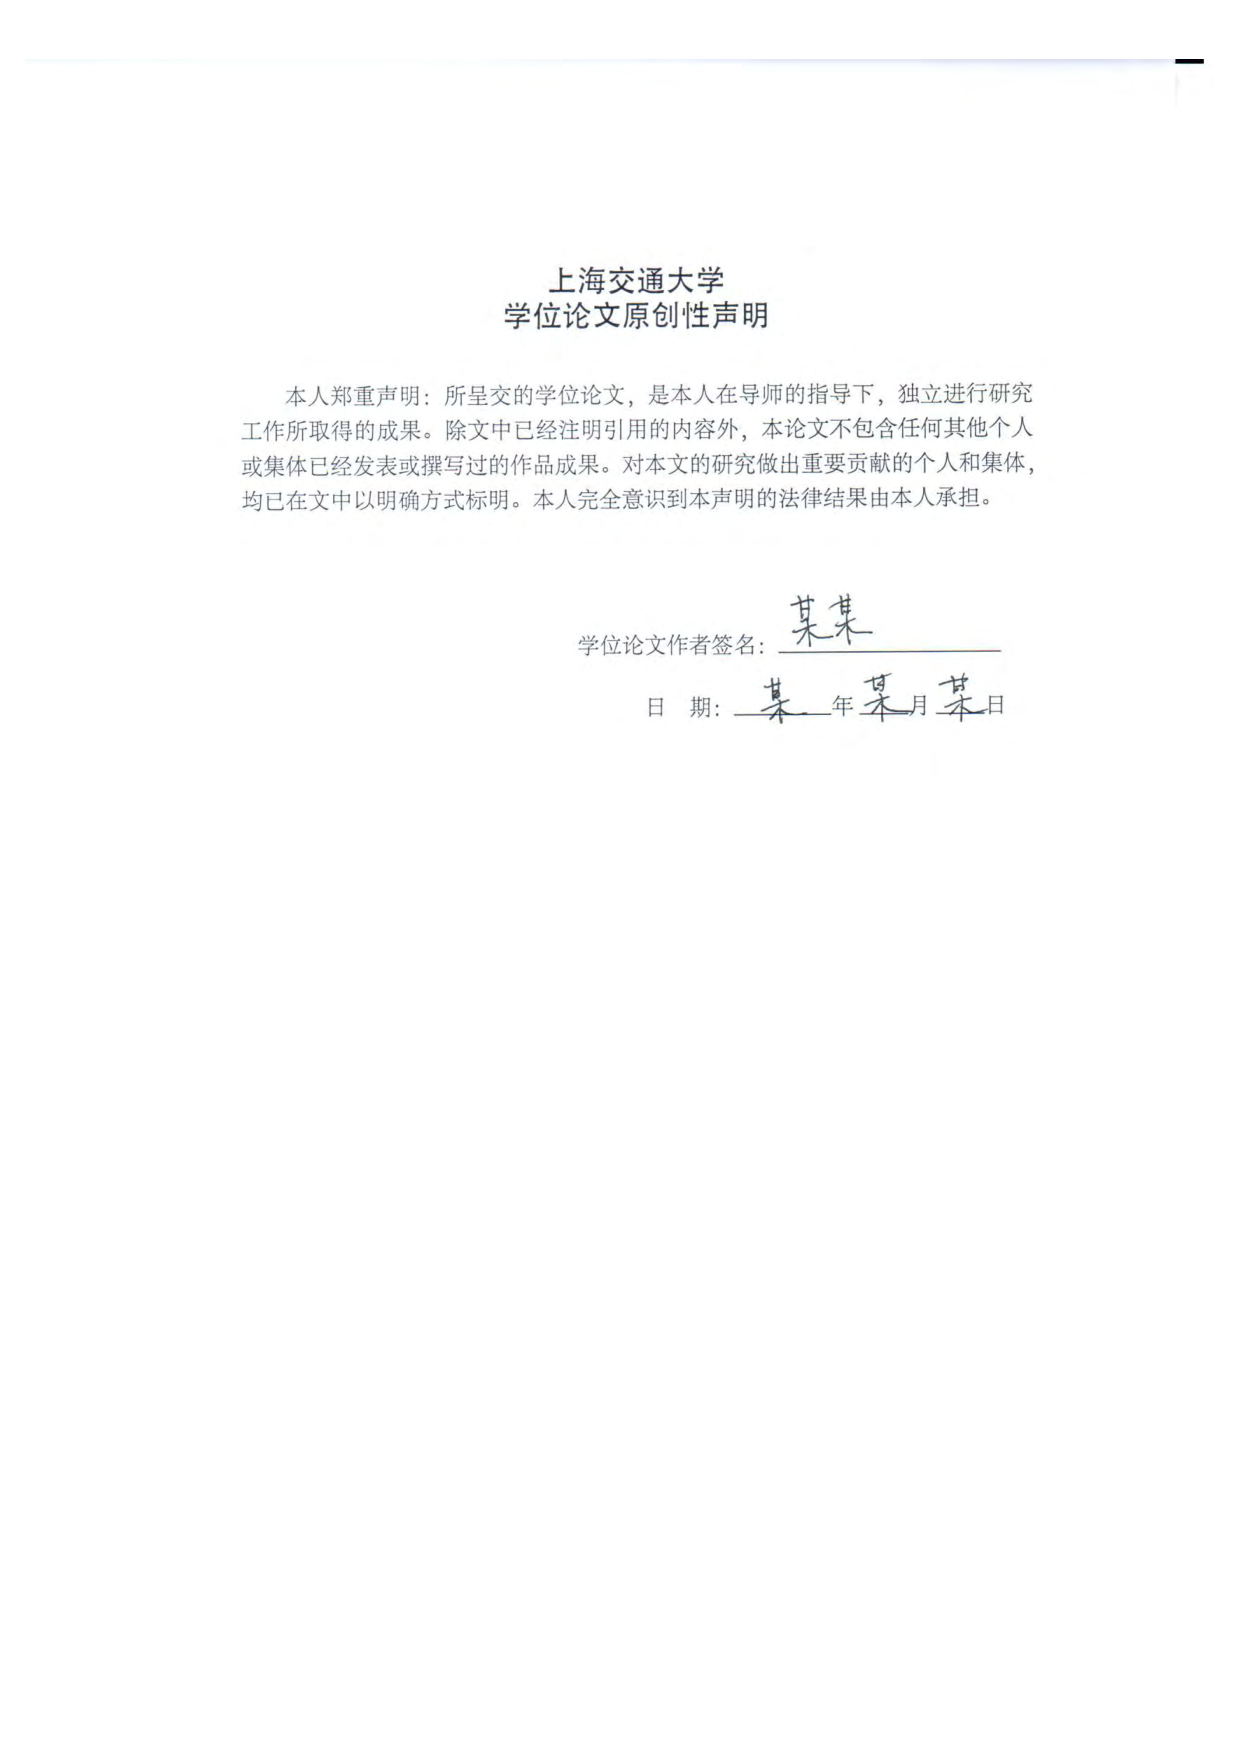
\includepdf{pdf/original.pdf}
	\cleardoublepage
	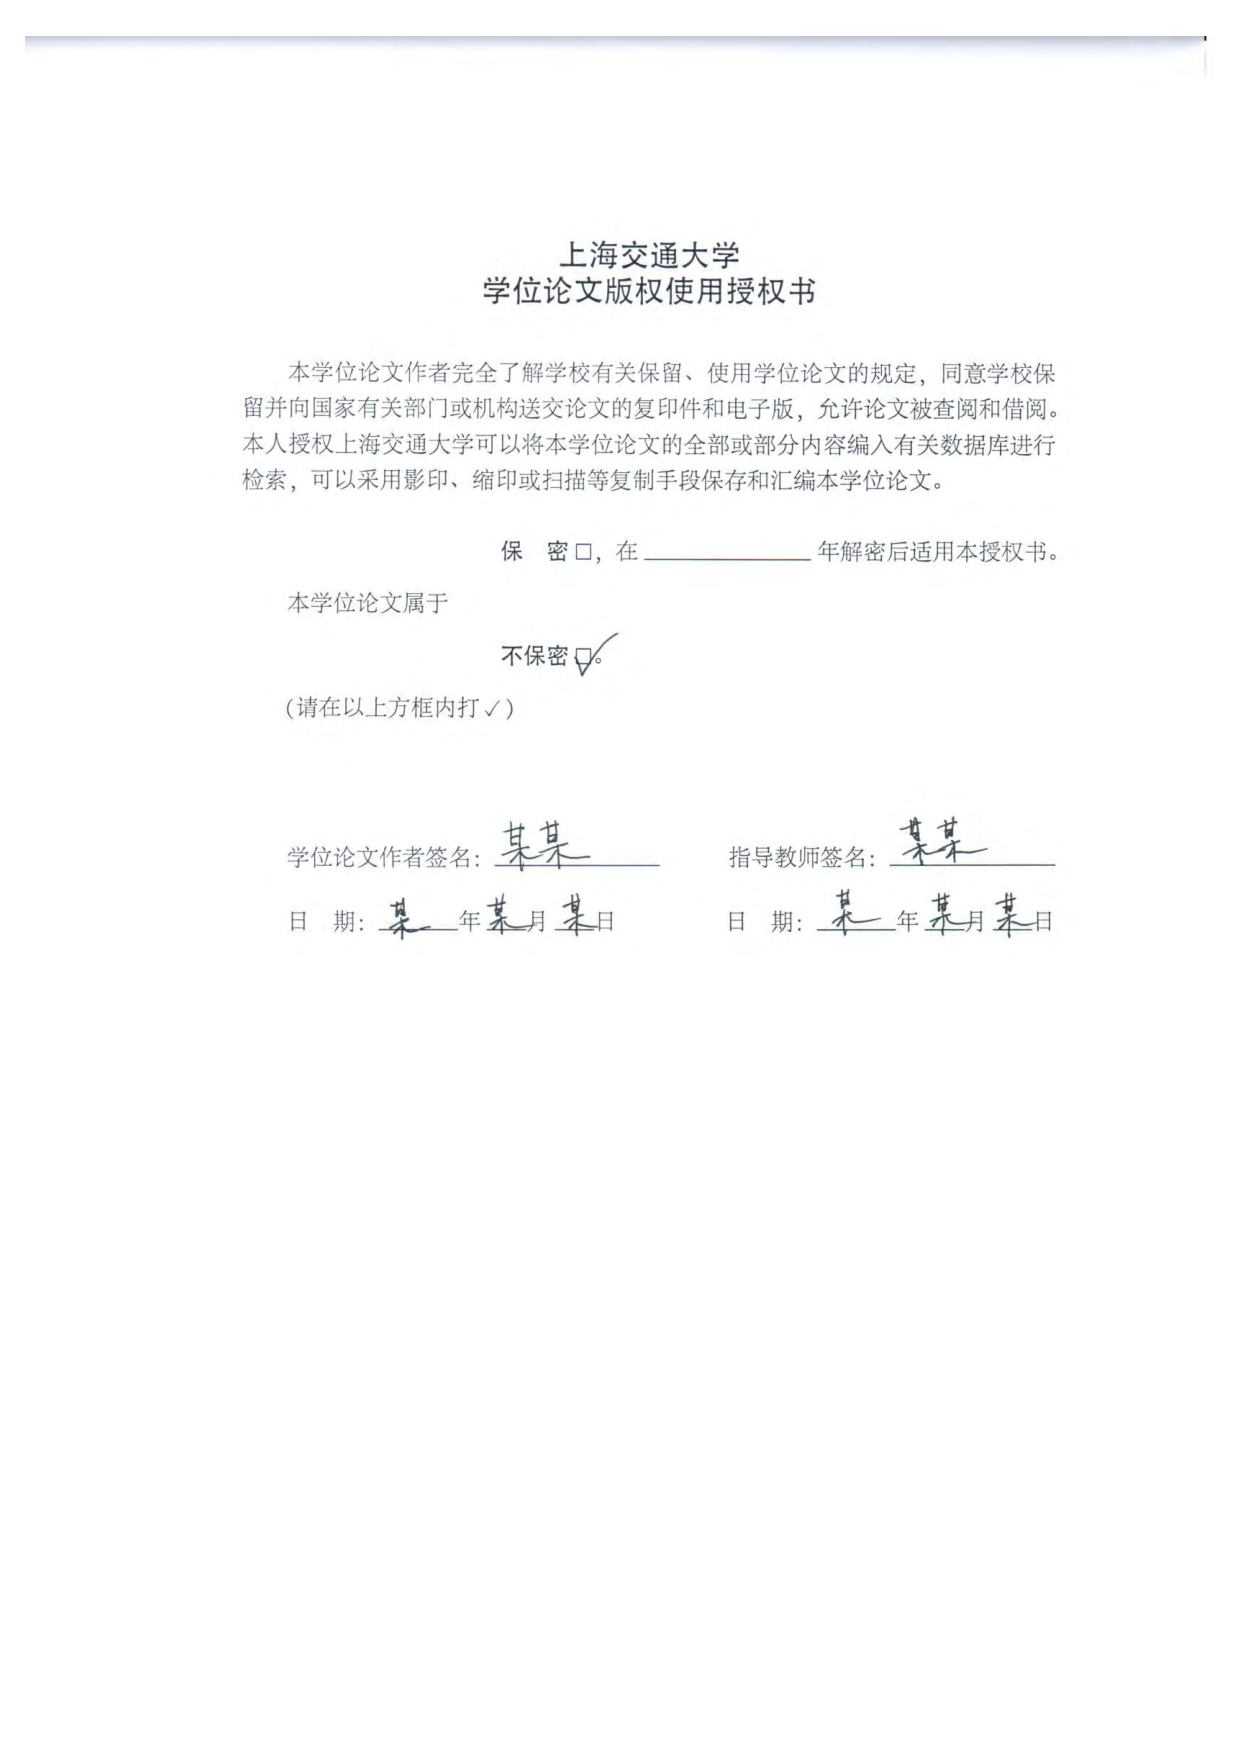
\includepdf{pdf/authorization.pdf}
	\cleardoublepage
\else
	\makeDeclareOriginal
	\makeDeclareAuthorization
\fi
\makeatother


\frontmatter 	% 使用罗马数字对前言编号

%% 摘要
\pagestyle{main}
%# -*- coding: utf-8-unix -*-
%%==================================================
%% abstract.tex for SJTU Master Thesis
%%==================================================

\begin{abstract}
时钟同步问题来源于工业中分布式系统的发展和实时性任务的需求,核心问题是通过同步方法来实现各个子系统之间的时钟一致性,传统的GPS同步方法和NTP(网络时钟同步协议)等协议由于价格昂贵、同步精度差等原因满足不了工业需求,IEEE1588精确时钟同步协议协议是目前时钟同步领域最好的同步方法,不过其在实际使用中由于链路延时等因素影响难以达到亚微秒甚至纳秒同步精度以及无法保证从时钟的稳定性。

本文从统计角度出发,对链路延时、时钟伺服系统及时钟频率漂移补偿进行深入研究,旨在提供一种系统性的统计方法来提高IEEE1588时钟同步系统精度及稳定性,主要工作如下:

(1) 通过对链路延时成分进行数学特性分析,并从统计角度提出动态阈值法与基于固定时间窗的实时监控算法等以提高同步精度;

(2) 在时钟伺服系统中,针对链路时延的阶跃突变干扰采用多模型PID控制策略,以优化从时钟的稳定性,减少从时钟的频繁抖动以保证整个系统的平稳运行;

(3) 对于时钟频率漂移问题,通过监测PTP报文样本是否发生链路堵塞等来进行报文过滤,只选取正常链路传输的PTP样本来进行校正,从而提高频率偏差计算的准确度;

(4) 通过对比边界时钟与透明时钟差异性来对统计算法进行调整,以使本文所提算法能够应用到透明时钟场合中;

(5) 通过stateflow时钟同步仿真系统进行仿真分析。仿真结果表明上述算法不仅能够提高时钟同步系统对多种链路延时抖动的适应性,还能提高整个系统的同步精度和稳定性。

\keywords{\large 时钟同步 \quad 统计算法 \quad 频率补偿 \quad 时钟伺服系统 \quad  \quad stateflow}
\end{abstract}

\begin{englishabstract}

Time synchronization problem originates from the requirement of developing distributed system and real-time tasks. The core problem is to achieve the time consistency among all the subsystems through time-synchronization method. The traditional GPS method and NTP protocol are not able to meet current industrial demand due to their high-cost and unpredictable message latency. Currently, IEEE1588 protocol is the best choice for time-synchronization problem, However, it often cannot achieve the precision level of sub-microsecond or nanosecond and it's not able to guarantee the stability of slave clock in the industrial reality.

From the perspective of mathematical statistics, the objective of this paper is to promote a systematically statistical method to improve the time-synchronization precision and stability. The contributions are shown in the following.

(1) Through the mathematical analysis for transmitting message latency, I decomposed latency into inherent jitter, temporary latency mutation and persistent latency change. In order to improve accuracy, dynamic threshold method and fixed-window real-time detection method are promoted.

(2) In clock servo system, multi-model PID controller strategy is promoted for improving the slave-clock stability when step-mutation occurs. So slave clock system will become more smooth due to the less jitter.

(3) By filtering PTP messages based on the detection of link blocking, qualified PTP messages will be choosed for calcuation of master-to-slave frequency offset.

(4) By comparing boundary-clock with transparent-clock, the statistics methods are promoted in order to make our statistical methods able to be applied into the occasion of transparent-clock device.

(5) Based on stateflow time-synchronization simulation system, all the promoted methods above get validated and verified. The simulation results show us those methods above can improve the adaptive ability of time-synchronization system for multiple types of latency changes, and the synchronization precision and stability of whole system as well.

\englishkeywords{\large clock synchronization,  statistical method, frenquency compensation, clock servo, stateflow}
\end{englishabstract}



%% 目录、插图目录、表格目录
\tableofcontents
\listoffigures
\addcontentsline{toc}{chapter}{\listfigurename} %将插图目录加入全文目录
\listoftables
\addcontentsline{toc}{chapter}{\listtablename}  %将表格目录加入全文目录
% \listofalgorithms
% \addcontentsline{toc}{chapter}{代码索引}  %将表格目录加入全文目录

% %# -*- coding: utf-8-unix -*-
\chapter{主要符号对照表}
\label{chap:symb}

\begin{longtable}{rl}
$\epsilon$     & 介电常数 \\
 $\mu$ 		& 磁导率 \\
 $\epsilon$     & 介电常数 \\
 $\mu$ 		& 磁导率 \\
 $\epsilon$     & 介电常数 \\
 $\mu$ 		& 磁导率 \\
 $\epsilon$ 	& 介电常数 \\
 $\mu$ 		& 磁导率 \\
 $\epsilon$     & 介电常数 \\
 $\mu$ 		& 磁导率 \\
 $\epsilon$     & 介电常数 \\
 $\mu$ 		& 磁导率 \\
 $\epsilon$     & 介电常数 \\
 $\mu$ 		& 磁导率 \\
 $\epsilon$ 	& 介电常数 \\
 $\mu$ 		& 磁导率 \\
 $\epsilon$     & 介电常数 \\
 $\mu$ 		& 磁导率 \\
 $\epsilon$     & 介电常数 \\
 $\mu$ 		& 磁导率 \\
 $\epsilon$     & 介电常数 \\
 $\mu$ 		& 磁导率 \\
 $\epsilon$ 	& 介电常数 \\
 $\mu$ 		& 磁导率 \\
 $\epsilon$     & 介电常数 \\
 $\mu$ 		& 磁导率 \\
 $\epsilon$     & 介电常数 \\
 $\mu$ 		& 磁导率 \\
 $\epsilon$     & 介电常数 \\
 $\mu$ 		& 磁导率 \\
 $\epsilon$ 	& 介电常数 \\
 $\mu$ 		& 磁导率 \\
 $\epsilon$     & 介电常数 \\
 $\mu$ 		& 磁导率 \\
 $\epsilon$     & 介电常数 \\
 $\mu$ 		& 磁导率 \\
 $\epsilon$     & 介电常数 \\
 $\mu$ 		& 磁导率 \\
 $\epsilon$ 	& 介电常数 \\
 $\mu$ 		& 磁导率 \\
 $\epsilon$     & 介电常数 \\
 $\mu$ 		& 磁导率 \\
 $\epsilon$     & 介电常数 \\
 $\mu$ 		& 磁导率 \\
 $\epsilon$     & 介电常数 \\
 $\mu$ 		& 磁导率 \\
 $\epsilon$ 	& 介电常数 \\
 $\mu$ 		& 磁导率 \\
 $\epsilon$     & 介电常数 \\
 $\mu$ 		& 磁导率 \\
 $\epsilon$     & 介电常数 \\
 $\mu$ 		& 磁导率 \\
 $\epsilon$     & 介电常数 \\
 $\mu$ 		& 磁导率 \\
\end{longtable}
 % 主要符号、缩略词对照表

\mainmatter	% 使用阿拉伯数字对正文编号

%% 正文内容
\pagestyle{main}
%# -*- coding: utf-8-unix -*-
%%==================================================
%% chapter_1.tex for SJTU Master Thesis
%%==================================================

\chapter{概述}
\label{chap:intro}
随着当前网络通信与计算机技术的不断发展,在工业领域中越来越多的基于网络的分布式系统得到了应用。而随着这些系统的物理范围不断扩大,也为了保证分布式网络系统能够实现精确的数据采集、运行控制等实时性任务,工业中对于各个分布式节点的时间同步精度提出了极为严格的要求,尤其是在大多数以工业以太网为基础的控制系统中,已经逐渐对同步精度提出了微秒级甚至纳秒级别的要求。但是,由于实际测控设备之间固有的时钟差异和时钟数据在网络传输中的随机延时,而且现场设备会由于温度变化、电磁干扰、振荡器老化等多种原因而使得自身时钟并不稳定,使得时间误差随时间不断累积,严重破坏了如变电站、电力监控系统等对时钟同步严格的工业应用。因此,必须追求一种更加有效且高精度的时钟同步技术来提高系统内部节点之间的时钟同步精度。

\section{工业领域中时钟同步的技术现状}
时钟同步即保证工业系统内各个节点的时钟能够保持一致,即维护一个全局一致的物理或逻辑时钟,使得系统各节点中与时间有关的信息、时间及行为有一个全局一致的解释\supercite{1}。
常说的时钟同步,主要包含了时刻同步和时间间隔一致。时刻即表示连续流逝时间的某一个瞬间,而时间间隔是指两个时刻之间的间隔长度。所以,时钟同步主要包括频率同步和相位同步两个方面:
\begin{itemize}[noitemsep,topsep=0pt,parsep=0pt,partopsep=0pt]
	\item 频率同步:指各从时钟自身运行的计数器频率保持相同平均速率。通过频率同步可以保持所有节点以相同的计数频率运行,从而极大减小时钟误差根源,降低了累积时钟误差。频率同步必须依靠接受连续的时钟信息才能计算出真实的频率并对自身作出调整。
	\item 相位同步:指对频率的积分。通过将时钟的相位量化,赋予数值表示,就是时刻。相位同步可以接受离散的时间信息来调整本地时钟。
\end{itemize}
所以说,时钟同步主要是完成对时和守时这两个功能,所谓“对时”,就是通过不定期的对表操作,来将本地时钟的相位与远程节点相位进行同步;守时就是保持频率一致,尽可能的让本地节点和远程节点的时间间隔偏差在一个允许的范围内。

在工业领域时钟同步技术不断发展,主要使用GPS、包时钟同步以及精确时钟同步等时钟同步技术。

\subsection{GPS同步技术}
如超高压变电站等工业系统对于时间同步精度的要求非常高,例如变电站运行人员实时监控电网运行,一旦发生事故后的故障分析,这些都需要统一的时间基准。而以全球定位系统GPS作为时间基准,可以提供非常高的同步精度(达到50ns),而且这种方式不依赖通络的数据负载,直接传递频率和相位信息,让整个系统保持极高的同步性能。然而,这种方式也存在自身弊端。
\begin{itemize}[noitemsep,topsep=0pt,parsep=0pt,partopsep=0pt]
	\item GPS不适用于室内节点,存在难以选址和安装的问题,这使得GPS同步技术的人力成本增大。
	\item GPS设备本身价格昂贵,而且人们一般会选取高昂的晶振用作备用时钟,以保持系统的安全性。而且若GPS设备大量使用,可想而知后期的更换升级的费用也会十分高昂。
	\item 由于美国政府从未对GPS信号的质量及使用期限给予任何承若何保证,而且美国政府还具有对特定地区GPS信号严重降质处理的能力,所以大量使用GPS会存在严峻的国防安全隐患。
\end{itemize}

\subsection{包时钟同步技术}
所谓包时钟同步技术ToP(Timing over Packet),就是利用分组网络来传递时间信息,而所传递的时间报文也有多种。
\begin{itemize}[noitemsep,topsep=0pt,parsep=0pt,partopsep=0pt]
	\item  NTP(Network Time Protocol)协议全称是网络时间协议,主要用来使互联网上计算机保持时间同步,一般而言,NTP可以提供1-50ms的可靠时间源。另外,SNTP(Simple Network Time Protocol)简单网络时钟同步协议也是较为主流的时间同步协议,它能提供接近1ms的同步精度。然后这两种协议比较容易受到网络突发报文的影响而使得同步精度降低。
	\item PTP(Precise Time Protocol)精确时间同步协议,来自于IEEE1588协议标准。该协议第一版于2002年推出,具备亚微秒级的同步精度,允许同时传递频率和相位信息。第二版于2008年公布,缩短并统一了报文长度,并且引入了透明时钟机制。具备更高的时间同步精度。
\end{itemize}

结合对当前所有同步技术的综合分析可以看出,由于GPS严重的国防安全隐患和高昂的使用成本使得人们难以大规模应用这种同步技术,而NTP协议主要应用于互联网中保持计算机时间同步,其精度只能达到毫秒级别,同样不适用于对同步精度要求非常高的工业系统中。而PTP同步技术从实现的简单性、精度要求和稳定性方面都能够很好的满足现如今分布式系统对时间同步精度的要求,因此,本文也选取PTP为主要研究对象。

\subsection{精确时钟同步技术}
应用于网络测量和控制系统的精确时钟同步技术是基于IEEE1588标准,也称作PTP协议(Precision Clock Synchronization Protocol)。

自1995年以太网中数据传输速度从10Mb/s提高到100Mb/s后,计算机网络领域一致在尝试解决网络设备时钟同步问题,随后开发出了一套同步协议--网络时间协议NTP(Network Time Protocol)--来提高网络设备的同步性能。虽然在不断发展中,NTP协议同步精确度不断提高达到200$\mu$s,但是,面对同步精度要求越来越高的网络实时通信、测量仪器与工业控制领域,NTP难以达到它们的要求。

随后,网络精密时钟同步委员会于2002年在IEEE标准委员会的支持下,推出了IEEE1588时钟同步标准。该标准推出后迅速在Ethernet/IP等基于以太网的总线中得到采用。该协议采用了主从时钟方案,利用报文传递时间信息,基于网络链路的对称性和延时测量技术,来实现主从时钟的频率、相位精确同步。

在2008年,该委员会继续发布了IEEE1588第二版。在第二版标准中,实现了亚微秒级的时钟同步,可以用于军事和实际的测试测量中。而且提供了更为灵活的同步周期、改进了时间戳的表示方法、解决了主时钟容错性能差的问题、提高了网络拓扑变化的适应性。另外,该版本中还引入了透明时钟,增加了端延时机制,有助于明显提高同步精度。

PTP协议主要针对分布式网络系统中的精确时钟同步问题,它能够将系统内部各个独立时钟同步到一个统一的时钟标准上,而且消耗的网络和本地资源非常有限,并带来较高的时钟同步精度。如果硬件时钟能够提供硬件级别的时间戳标记功能,那么其同步精度能够达到亚微秒级别。而且PTP协议实现起来成本很低,也非常方便后期的维护工作。

PTP协议与其他时钟同步协议如NTP/SNTP相比,具备如下几个特点:
\begin{itemize}[noitemsep,topsep=0pt,parsep=0pt,partopsep=0pt]
	\item PTP协议适用于局域网中支持组播报文发送的网络通信技术,这种特性决定了该协议非常适合在以太网中实现,不需要经过大的改动就可以在高精度的网络控制系统中运行。
	\item 可以实现亚微秒级别的同步精度,相比之下,NTP/SNTP最多只能达到毫秒级别。
	\item PTP协议所需要的网络资源和计算资源非常少,所以在实现起来消耗的成本不高。
\end{itemize}

随着IEEE1588协议的不断发展与实践,不仅在测试与测量控制、工业自动化领域广泛应用了该协议,而且随后的军事应用、分组通信和电力系统等多个领域也开始逐步将该同步方法应用进去。在国外,2015年3月在TI推出的高性能多核架构KeyStone中,提供了两个硬件功能来支持IEEE1588:记录时间戳,发送同步脉冲。其中KeyStone1支持two step的时间戳模式,同时也能支持1588协议中规定的PTP报文解析,在国内,2014年12月,OPWILL发布了基于PTN协议分析仪的IEEE1588v2PTP和SyncE测试选件,为运营商提供关键的网络定时和频率同步测试服务来分析全新的IEEE1588v2 PTP和同步以太网(SyncE)协议,从而为运营商的移动回传和LTE测试提供超高性价比测试解决方案。

\section{精确时钟同步技术应用现状}
根据IEEE1588协议内容,系统时钟同步精度应该能够达到亚微秒级\supercite{2}。然而,在实际的应用中,即使严格按照协议标准的内容来实现,仍然难以达到这样的同步精度。例如Padova大学曾严格按照协议标准,实现了一套完整的IEEE1588同步系统\supercite{3},但是在运行中发现同步精度最高只有100微秒,和预期的同步精度还有很大的差距,更何况在工业现场中,更加复杂的工业环境使得同步精度更加难以保证。

首先,IEEE1588协议的同步原理是采用了主从时钟通过时间戳报文来传递时间信息,并通过估计链路延时来计算最终的时间误差并予以校正。然后,通过对1588协议的深入分析及对现场应用情况的深入了解,可以发现以下因素严重破坏了1588实际运行的同步精度。

(1) 时间戳精确度

首先,1588协议的核心就是通过主从时钟对外发布包含时钟信息的报文来实现所有从时钟向主时钟同步。例如在同步过程中,主时钟会对外发送sync报文,该报文中标记的时间戳在理想情况下应该是报文离开主时钟的一瞬间的时间,但是在实际运行中,由于很多时间戳是在物理层之上标记的,报文被标记时间戳后仍会在协议栈中有短暂滞留,这样导致了发送时间戳的不准确,最终破坏了从时钟的同步计算精度。

(2) 链路不对称性

通过分析1588协议可以看出,从时钟在计算主从时钟偏差时会假设报文传输的往返路径对称,即Master To Slave Delay 和 Slave To Master Delay相等,并据此来求得最终的offset值。严格来讲,这种假设并不成立。首先由于网络传输过程要经过中间节点如交换机等设备,报文在进入这些设备的协议栈会发生排队和堵塞的情况,而这些情况所导致的链路延时变动是无法预知的;另外,报文传输的拓扑结构也并非一成不变的,一旦拓扑结构发生变化,就意味着往返路径可能有极大的不同。这些都是实际运行中链路固有的不对称性表现,所以,如果只是简单按照1588协议中假设路径对称,那么势必会带来不可忽视的误差。

(3) 网络延时固有抖动

由于1588协议中的报文需要在网络环境下进行传输,而在复杂的网络环境下,报文传输的时间一定会带有随机的抖动漂移,也就是说,即使网络负载良好,拓扑结构也不发生变动的情况下,网络延时仍然会有自身的随机抖动。如果对于这些抖动不进行处理,那么就会导致从时钟不断处于波动之中,甚至有可能导致从时钟系统不稳定。

(4) 主从时钟源晶振漂移

首先,IEEE1588协议的主从时钟偏差的计算方式是假定主从时间偏差值在短时间内是保持不变的。然而真实的情况是,主时钟在发送Sync报文时的偏差值Offset\_1与从时钟最后接收Delay\_Respo报文时的偏差值Offset\_2是不完全一致的,所以最终计算出来的offset并不完全等于真实的Offset\_2。所以这会导致同步精度变差。

(5) 从时钟校正策略

常规的对从时钟校正策略有直接校正和PI控制器校正,其中,直接校正能够快速对从时钟校正,在最短时间内实现时钟同步,然后,一旦offset值计算中存在较大偏差,那么从时钟将处于不断的快速波动当中,这会严重破坏从时钟的同步性能,甚至可能导致从时钟无法稳定。PI控制器是一种较为典型而简单的控制方法,能够保证从时钟较为处于较为稳定的状态,但是,简单的PI控制器并不能考虑到延时的波动对从时钟带来的影响,所以也无法达到很好的控制效果。

当前针对上述所提出的问题,工业界对1588协议进行了深入研究并取得了一定的研究成果。

(1) 时间戳准确度研究现状

为了提高时间戳准确度,尽量使得报文中的时间戳直接来自物理层以可以减少报文在协议栈的停留,2007年推出了首个可以在以太网收发器上集成IEEE1588协议的芯片-DP83640\supercite{4},该芯片能够将时间戳标记点葱原来的应用层下移到数据链路层和物理层之间,从而降低网络流量及协议栈对报文传输延时的影响。又比如,2015年3月TI推出的Keystone架构也同样能够支持物理时间戳标记\supercite{5}。

(2) 链路不对称性研究现状

针对链路延时中的不对称性问题,李学桥层提出对主从路径延时和从主路径延时进行加权求平均的方法,其中权值来自于同步报文与延时请求报文的周期比\supercite{6}。在李帅等学者的文献\parencite{7}中提出了一个扩展时钟同步方法来计算不对称路径下的时间偏差。另外,当前主要的解决方法有通过类似透明时钟来记录报文在中间节点的传输时间,并在从时钟处减去传输时间来计算主从偏差。但这种方式在2008年才提出,目前并未得到广泛应用,它不仅会受时间戳精度影响,而且现有大多数同步系统仍然采用的是早期的边界时钟。所以当前并不具备很好的应用价值。在C. Lei的文字\supercite{57}中采用了自适应滤波算法,该算法能较好的进行滤波,但由于不能对历史纪录进行实时分析,从而无法检测持久性的时延变化。

(3) 网络延时固有抖动研究现状

Jayesh Chhapekar在2012年发表的一篇文章中对IEEE1588数据包的包延时抖动进行数学分析和建模,并以此来观察数据包延时的概率是如何变化的\supercite{8}。但是在真实的工业环境中,由于网络的复杂性和时变性,很难用某个概率分布来拟合固有抖动,所以也很难取得良好的消除抖动效果。文献\parencite{9}中设计了运用卡尔曼滤波算法来计算主从时钟偏差同样有助于减少固有抖动带来的影响。

(4) 从时钟校正策略研究现状

当前普遍方法是采用PI控制器进行校正,如文献\parencite{10}中对PI控制器参数选择进行了评估,但是没有详细研究具体的应用方法。另外由于网络的时变性,无法用固定的参数来控制从时钟,那样会带来很差的自适应性和鲁棒性。除此之外,文献\parencite{11}对PID控制器在时钟同步中的应用进行深入研究,并且采用了经验法来对PID参数进行整定,但该文缺陷是没有把系统参数发生变化情况下的参数调整考虑进去。文献\parencite{12}利用模糊控制算法来估算时钟偏差,这种方法适合于时钟同步周期较大时,但是如果同步周期太大,网络的不确定性干扰加剧,使得模糊控制的效果变差。

\section{本文研究内容}
越来越多的工业领域对时钟同步精度提出了非常高的要求,而传统的NTP和GPS由于使用成本高昂或者同步精度不够而无法满足对应的需求。相较而言,IEEE1588精确时钟同步协议由于其易用性、成本低、精度高等多种优秀特性已经广泛应用于多种工业时钟同步场合,而且随着IEEE1588-2008的推出,其理想精度甚至可以达到亚微秒级,这预示着IEEE1588协议有着极高的研究价值。另外,在IEEE1588协议的实际应用过程中,通过深入研究分析发现了协议本身存在的多种问题,例如未处理网络延时的不对称性及固有抖动,加之工业网络环境复杂,这使得IEEE1588协议在实际应用中无法达到非常理想的同步精度。而本文便是着手于影响同步精度的因素并通过深入分析来提出本文的解决方案。

\subsection{网络传输时延的随机性和不确定性}
在硬件提供高精度时间戳的情况下,网络传输延时误差成为了影响同步精度的最主要来源。因此,本文也着重考察对网络延时问题的解决方法。文章中将网络时延拆分成固有抖动漂移、暂时性时延突变和持久性时延变化,分别分析各种变化原因,并且从数学统计方法的角度出发,对固有抖动漂移提出基于最小二乘的时延估计方法,把历史时延数据作为样本序列,通过回归建模来进行时延估计,从而减小时延抖动或突变对同步精度带来的不良影响;对暂时性时延阶跃突变,提出动态阈值算法,通过限制阶跃噪声的大小来防止从时钟系统出现过大的振荡;对持久性时延变化,提出基于固定滑动时间窗实时检测的方法来及早发现持久性变化,并立即通过样本失效手段来快速消除持久性变化对样本序列及时延估计所带来的波动。基于以上所提出算法来保证时延的稳定性、准确性和可靠性。

\subsection{从时钟校正的控制策略}
为了提高从时钟稳定性,一般会采用时钟伺服系统来对从时钟进行控制,一般而言,会使用PID控制器来控制从时钟校正量,不过,通过对链路延时的分析,可以发现其中存在一种阶跃性延时。当一个进入稳态的从时钟遇到了阶跃性延时信号时,就会发生一定的抖动并慢慢收敛,这会导致从时钟的频繁调整,从而影响到整个系统的时钟变化。因此文中提出了多模型PID控制系统,通过对误差信号进行监控,当信号发生较大跳变时调整控制器以提高从时钟系统稳定性。

\subsection{统计方法在晶振源漂移及透明时钟中的应用}
由于IEEE1588中默认了一个假设:即认为主从时间偏差值在短时间内是保持不变的。而在实际情况下,由于主从时钟晶振不一致,这会导致主从时钟便差在实时变化中。这使得难以得到最真实的主从偏差值而无法精确校正。所以,文中将会从统计方法角度出发,针对主从时钟源漂移问题提出优化方法,以对从时钟晶振漂移进行补偿从二减小主从偏差的波动。另外,由于IEEE1588v2中引入了透明时钟的概念,为了能够将本文的统计方法应用到透明时钟中,下面会做出相关差异分析,并提出相关的处理方案。

\subsection{算法仿真与验证}
在文章后面,本文在深入研究所提出的多种时延统计优化算法的前提下,通过在自己搭建的基于stateflow的matlab仿真平台上,分别测试了上述所提两种算法。根据最终试验结果表现来观察所提算法对时钟同步系统的稳定性、鲁棒性和自适应性等当面的优化。

% \subsection{创新点}
% \begin{itemize}[noitemsep,topsep=0pt,parsep=0pt,partopsep=0pt]
% 	\item 基于统计策略的时延处理:针对时钟同步过程中的时延变化,当前的处理方法主要有对主从路径延时和从主路径延时进行加权求平均的方法,通过类似透明时钟来记录报文在中间节点的传输时间的方法,不过,这些方法并不能系统性的一次解决链路延时中存在的多种因素所带来的问题,且类似于透明时钟的方法也容易受到硬件限制而难以达到很好的效果。而本章节中提出的统计方法,提供了一个全新的能同时应对多种链路延时波动因素的思路,利用这种方法,可以很简便的应对固有抖动、暂时性时延突变和持久性时延变化三种情况。
% 	\item 基于多模型PID控制的时钟伺服系统:常规的时钟伺服系统是直接用普通PID控制器进行校正,不过,这种方法不能很好应对链路时延中存在的阶跃变化,因此,文中又提出了一种“多模型PID控制系统”,即通过对控制误差进行检测,一旦发现控制误差发生阶跃变化,就切换控制器,以防止从时钟发生较大抖动。这可以把持续的波动转变成一个瞬时性的“变化”,从而明显减小从时钟的频繁抖动,使整个系统更加稳定。
% 	\item 统计算法在晶振源频率补偿中的应用:常规的频率补偿是在一个时间段内直接把Sync报文的收发时间用来估算主从时钟的频率及差值以进行补偿。但是,这个时间段内很有可能发生链路延时的暂时性变化,即发生排队堵塞,导致有的Sync报文的传输时间很长,导致计算出来的频率有误差。而本文会通过对Sync样本进行处理,过滤掉发生时延突变的报文,只选取稳定传输的报文来进行处理。这样子可以确保频率计算的准确性。
% \end{itemize}

\section{论文安排}
本文的其它章节安排如下,

第二章介绍1588同步协议的运行原理,同时在最后介绍1588协议在实际运行中遇到的一些不可避免的问题,及对于这些问题的已有研究成果。

第三章从网络传输延时的角度来进行分析,并且提出结合数学统计与实时检测相结合的方法来保证延时数据的稳定性、准确性和可靠性。在该章节会首先对传输延时进行数学模型的建立,通过深入分析其特性可得到数学模型,然后依据模型特性,基于相关的数学统计方法,例如线性回归、固定时间窗等,提出符合模型特性的数学统计优化算法。其中,本文还会提出一套完整的滑动时间窗延时实时检测方案,用以区分暂时性延时和持久性延时,并在此基础上提出不同的处理方案。从而保证从时钟的稳定性。

第四章从统计角度出发,首先针对时钟伺服系统进行分析,然后为了应对其中的链路延时阶跃突变,文中提出了基于多模型PID控制的控制策略,以提高从时钟的稳定性;另外,针对主从时钟源晶振漂移问题,提出了相关的解决方案,以对从时钟晶振漂移进行频率补偿来减小主从偏差的波动。同时还将对统计算法在透明时钟的应用作出分析,并提出相关的实际应用方案。另外,该章还会利用自己搭建的时钟同步系统仿真平台,并在该平台上对本文中所提到的统计优化算法进行验证。根据仿真结果得出结论,并总结其中的不足之处。

第五章对全文进行总结和展望。

%# -*- coding: utf-8-unix -*-
%%==================================================
%% chapter_2.tex for SJTU Master Thesis
%%==================================================

\chapter{IEEE1588协议原理分析及相关研究}
\label{chap:1588_theory}
IEEE1588协议全名为:IEEE Standard for a Precision Clock Synchronization Portocol for Networked Measurement and Control Systems,也称为PTP精密时钟同步协议。PTP协议内部集成了多项分布式技术,如网络通信、局部计算和分布式对象等,对于所有支持多播局域网通信的分布式系统,尤其是以太网,都可以应用PTP协议来进行时钟同步。这可以在占用极少网络和本地计算资源的前提下,使得各类具有不同精确度、分辨率和稳定性的时钟同步且达到亚微秒级别的同步精度。

由于当今测控系统中越来越多的依赖分布式系统技术,而分布式系统的性能又极其依靠所有分布式节点之间的时钟同步精度。所以,一套优秀且能达到微秒甚至亚微秒级别的时钟同步协议显得尤为迫切,而IEEE1588协议的出现给这种需求带来了重要的影响,在相关领域也得到了非常快速的发展。

本章中会对IEEE1588时钟同步原理进行深入的分析研究,同时,本人也会对该协议中可能存在的一些严重问题进行分析,同时通过阅读文献来介绍关于这些问题的当今的一些研究理论成果,以期对IEEE1588协议原理及当前研究热点作一个较为立体而全面的分析。

\section{IEEE1588协议同步机制}
一般而言,IEEE1588系统是由PTP设备和非PTP设备结合而成的分布式网络化系统。IEEE1588协议主要介绍的是系统中的实时PTP设备之间的相互同步方案,使得所有的从时钟能够与自己的主时钟同步,而所有主时钟又能够和同一个Grand Master时钟同步,最终达到整个系统中所有时钟保持同步。

\section{时钟同步过程}
首先,每个ptp时钟会有多个端口,当系统启动时,会立即开始主从秩序建立过程。该过程中,每个端口会对外发送Announce报文,同时通过检查所收到的Announce报文中的相关信息来判定哪个端口适合成为主时钟,被判定为主时钟的端口则会定期对外发送Sync报文。如果,一个判定为主时钟的端口收到了一个来自于更好的主时钟的Sync报文,那么该主时钟则会立即将自身的主时钟状态切换为从时钟状态。当然,如果一个处于从时钟状态的端口认为自己比当前主时钟更加好,那么它可以将自己设置为主时钟状态,并对外发送Sync报文。当所有端口通过互相比较时钟特性并建立了各自的主从状态后,则意味着主从秩序完成建立。如果此时新加入了一个时钟,那么该时钟首先会等待来自某一主时钟的Sync报文,若在规定的时间内没有收到任何主时钟的Sync报文,那么该时钟则将自身设置为主时钟,直到发现一个更好的主时钟。

随后,则会进行时钟同步过程。该过程主要是主从时钟之间发送报文,使得每个从时钟计算出自身与主时钟之间的时钟偏差,并且对自身进行校正从而实现同步。首先主时钟会对外界进行周期性的Sync报文发送,多数情况下该报文会将离开主时钟的时间戳标记进去。当从时钟收到Sync报文后,则能够接受到发送时间戳并记录当前的接收时间戳。但是,仅仅依靠这两个时间戳还不能够计算出真实的主从偏差,因为对于从时钟而言它并不知道自身与主时钟之间的链路传输延时。所以,从时钟自身也会周期性向主时钟发送Delay\_Request报文,会通过接受主时钟回传的Delay\_Resopnse报文来共同计算出链路延时delay和主从偏差offset。最终利用offset对从时钟进行校正而实现同步。

下面,详细介绍主从建立过程中及时钟同步过程中所应用到的算法,并对算法进行分析。

\subsection{最佳主时钟算法}
\label{sec:1588_theory_bmc}
我们知道,ptp协议的核心是从时钟向主时钟同步从而最终实现整个系统时钟同步。所以,在真正的时钟同步之前,至关重要的一步便是建立全系统主从秩序,在该建立过程中,所有网络节点会通过“最佳主时钟算法(Best Master Clock Algorithm, BMC)”,选举出Grand Master Clock、主时钟、从时钟。其中,Grand Master Clock的精度最高,主时钟其次,从时钟最低。

下面进行简明扼要的最佳主时钟算法介绍。

当系统在启动之初,所有系统内部的时钟会对外发布Announce报文,该报文会包含自身时钟的与精度相关的特性。与此同时,所有时钟也会接受其他时钟发送过来的Announce报文,即接收到其他报文传递来的精度信息。

然后,每个端口内部会依据这些精度相关的数据集,在本地首先通过数据集比较算法,从而比较出两组数据的优劣,其中一组是时钟自身的缺省特性,另一组是来自外界其他时钟传递过来的数据。完成了数据集比较之后,会依靠比较结果继续执行状态决定算法。该算法会结合端口状态机规则及数据集比较结果来设置自身端口的主从状态。至此,每个时钟便已设置好了自身的主从状态,这其中最高级的主时钟便自动成为了Grand Master Clock。
\\
\\

具体拓扑结构可以参考下图:
\begin{figure}[!hbp]
  \centering
  \begin{minipage}[b]{0.6\textwidth}
    \captionstyle{\centering}
    \centering
    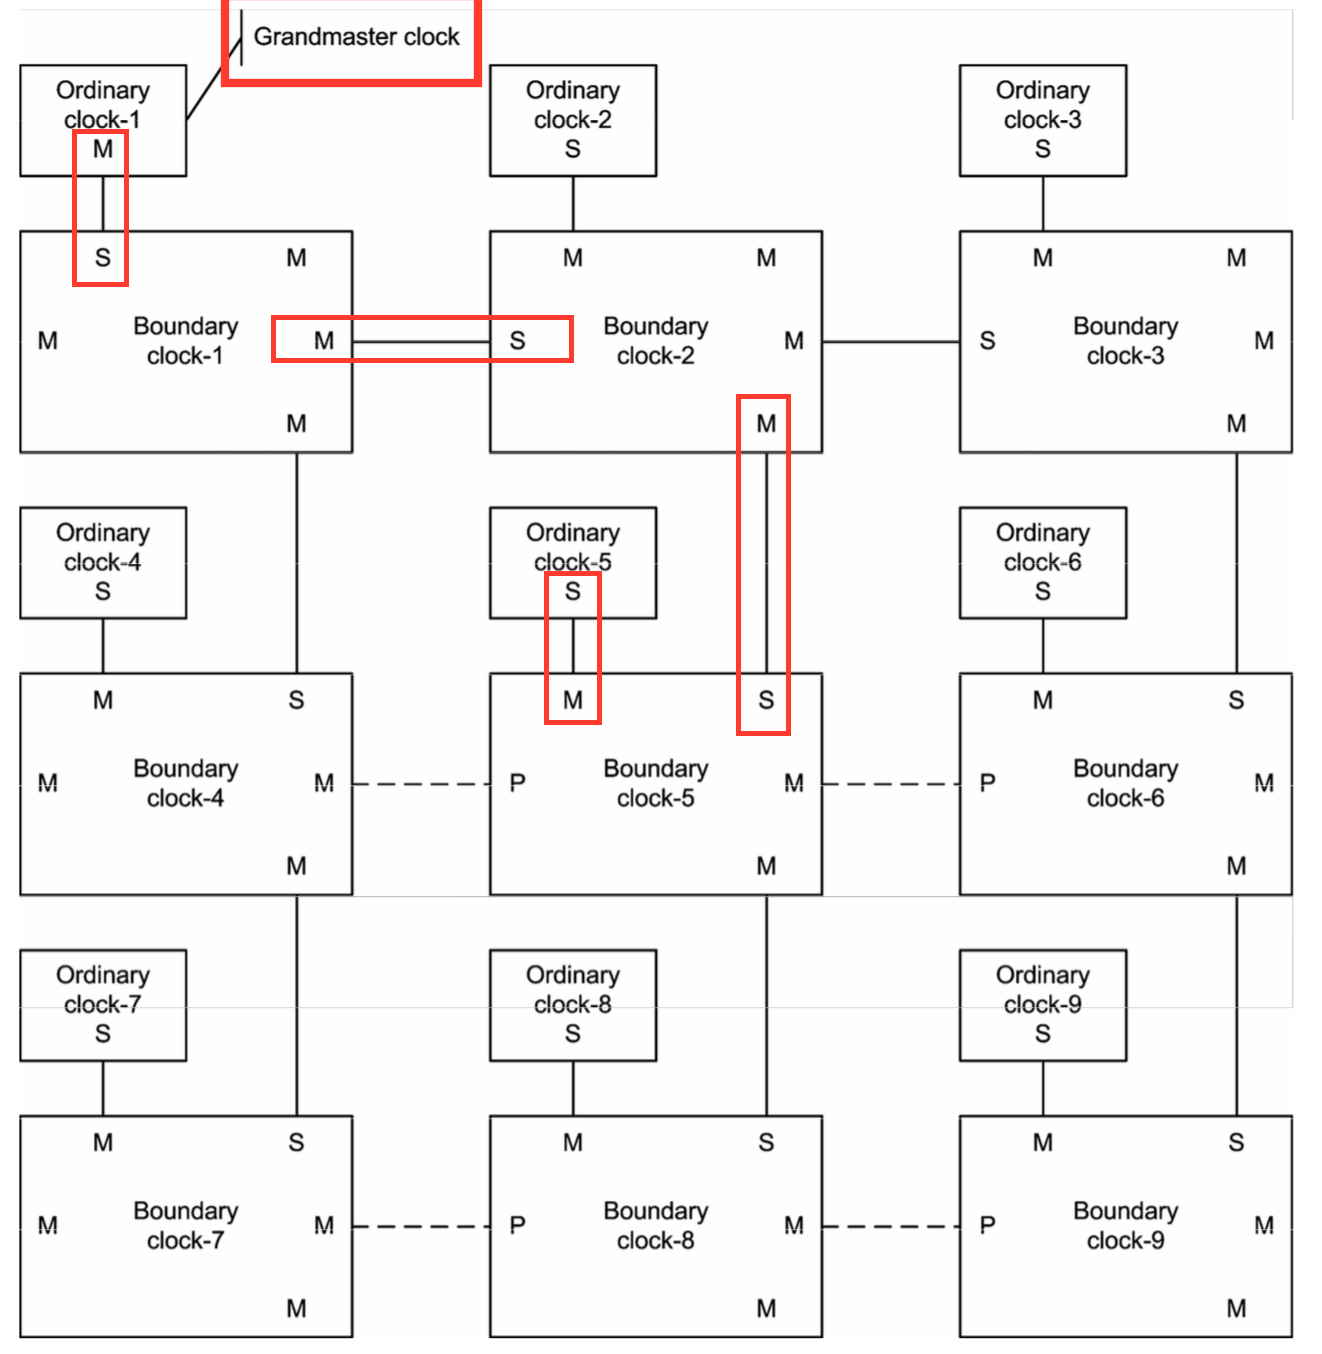
\includegraphics[width=10cm]{ptp_topo}
    \bicaption[fig:longcaptiongood]{PTP时钟同步拓扑结构}{PTP时钟同步拓扑结构}{Fig}{The topology of PTP Time-Sync System}
  \end{minipage}     
\end{figure}

\subsubsection{数据集比较算法}
数据集比较算法主要通过下列时钟属性来进行比较,且从上往下优先级逐渐降低:
\begin{enumerate}[noitemsep,topsep=0pt,parsep=0pt,partopsep=0pt]
	\item 优先权1(Priority 1):若某时钟被人工设置为优先权1,则自从成为主时钟;
	\item 层数(Stratum):总有有0 - 4级,层数越高则时钟等级越低,成为主时钟;
	\item 时钟标识符(Clock Identifier):即时钟精度,包括nature、expected accuracy和epoch,精度高的成为主时钟;
	\item 变量(Variance):即时钟稳定性,值越大表示稳定性越差,值小的成为主时钟;
	\item 距离(Distance):即指自身与外部主时钟之间的无力距离,离外部主时钟近的称为主时钟;
	\item UUID:代表节点唯一标识,UUID小的成为主时钟;
	\item 端口号码(Port Number):每个节点的数据集都包含一个端口号码,端口号码小的成为主时钟。
\end{enumerate}

在该比较算法中,会依次从上往下比较各个属性,只要发现一方的某个属性优于另一方,则立即成为主时钟,并停止数据集比较。当一个子网里各条路径的主时钟都进行了数据集比较算法,那么其中的最佳主时钟就称为了Grand master Clock。

可参考图\ref{fig:dataset_comparison_1}和\ref{fig:dataset_comparison_2}所示:

\begin{figure}[!hbp]
  \centering
  \begin{minipage}[b]{0.8\textwidth}
    \captionstyle{\centering}
    \centering
    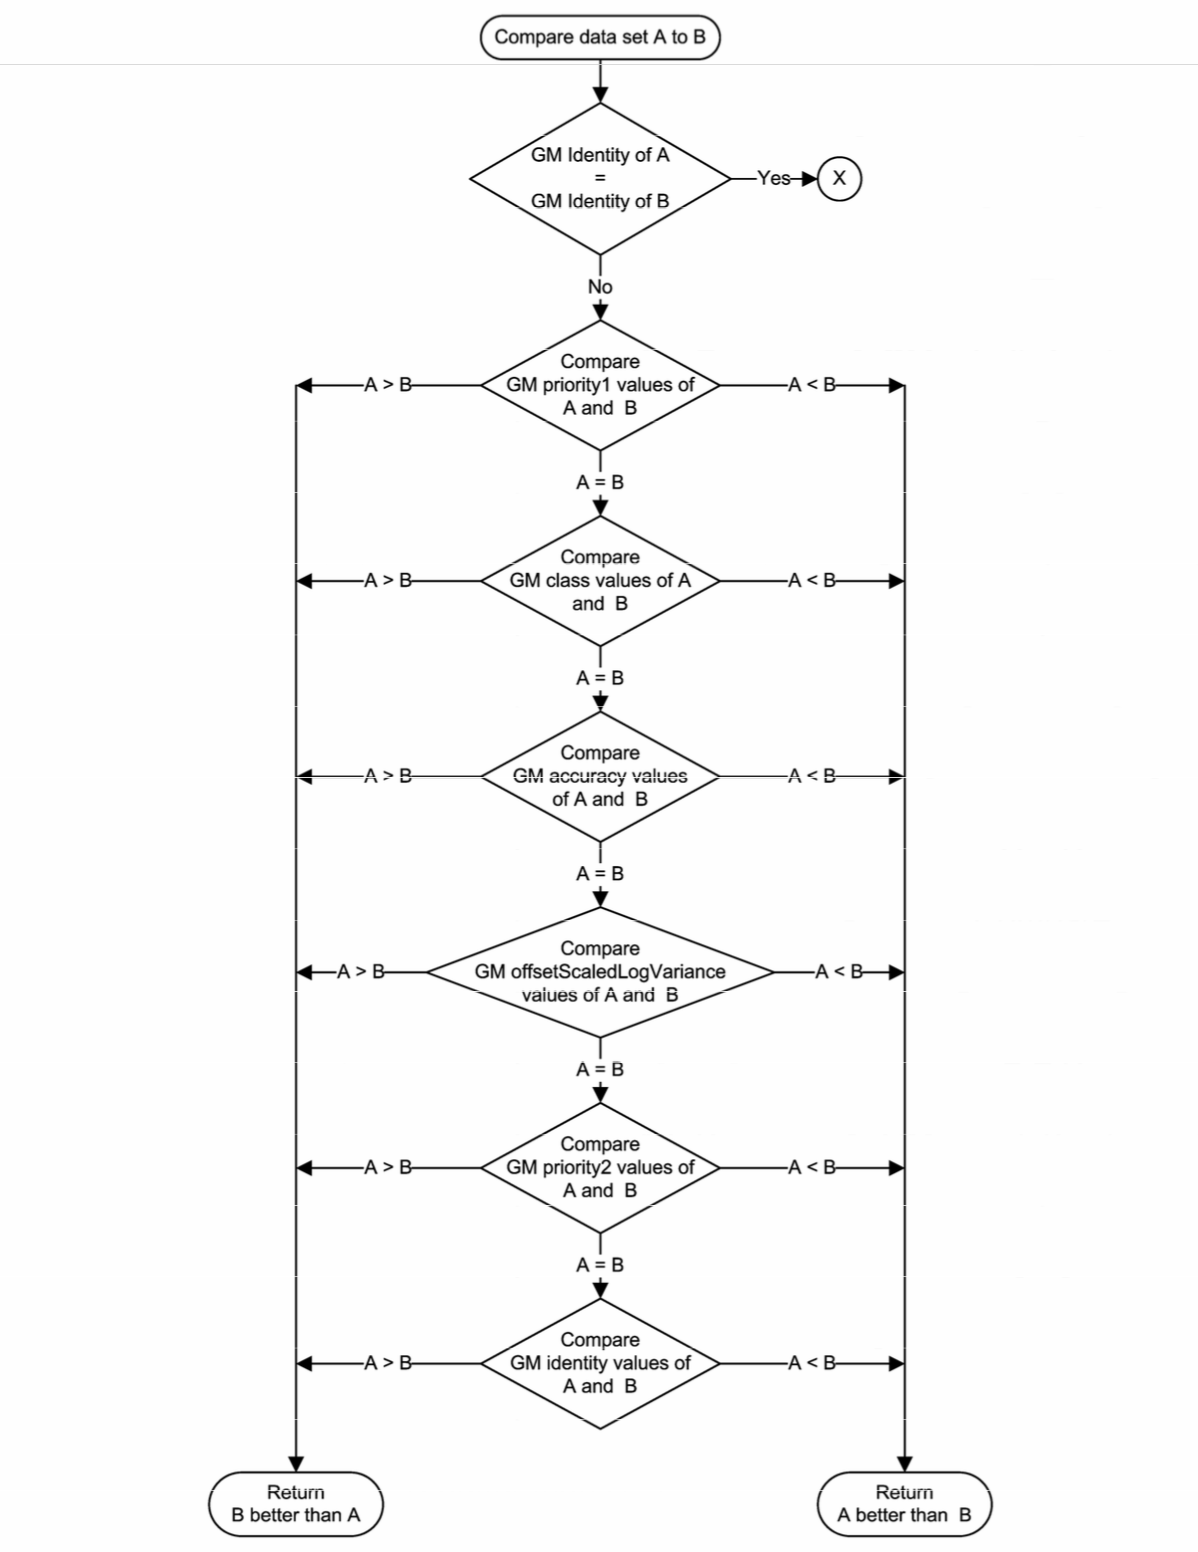
\includegraphics[width=12cm]{dataset_comparison_1}
    \bicaption[fig:dataset_comparison_1]{数据集比较算法Part1}{数据集比较算法Part1}{Fig}{The Dataset Comparsion algorithm Part 1}
  \end{minipage}     
\end{figure}

\begin{figure}[!hbp]
  \centering
  \begin{minipage}[b]{0.6\textwidth}
    \captionstyle{\centering}
    \centering
    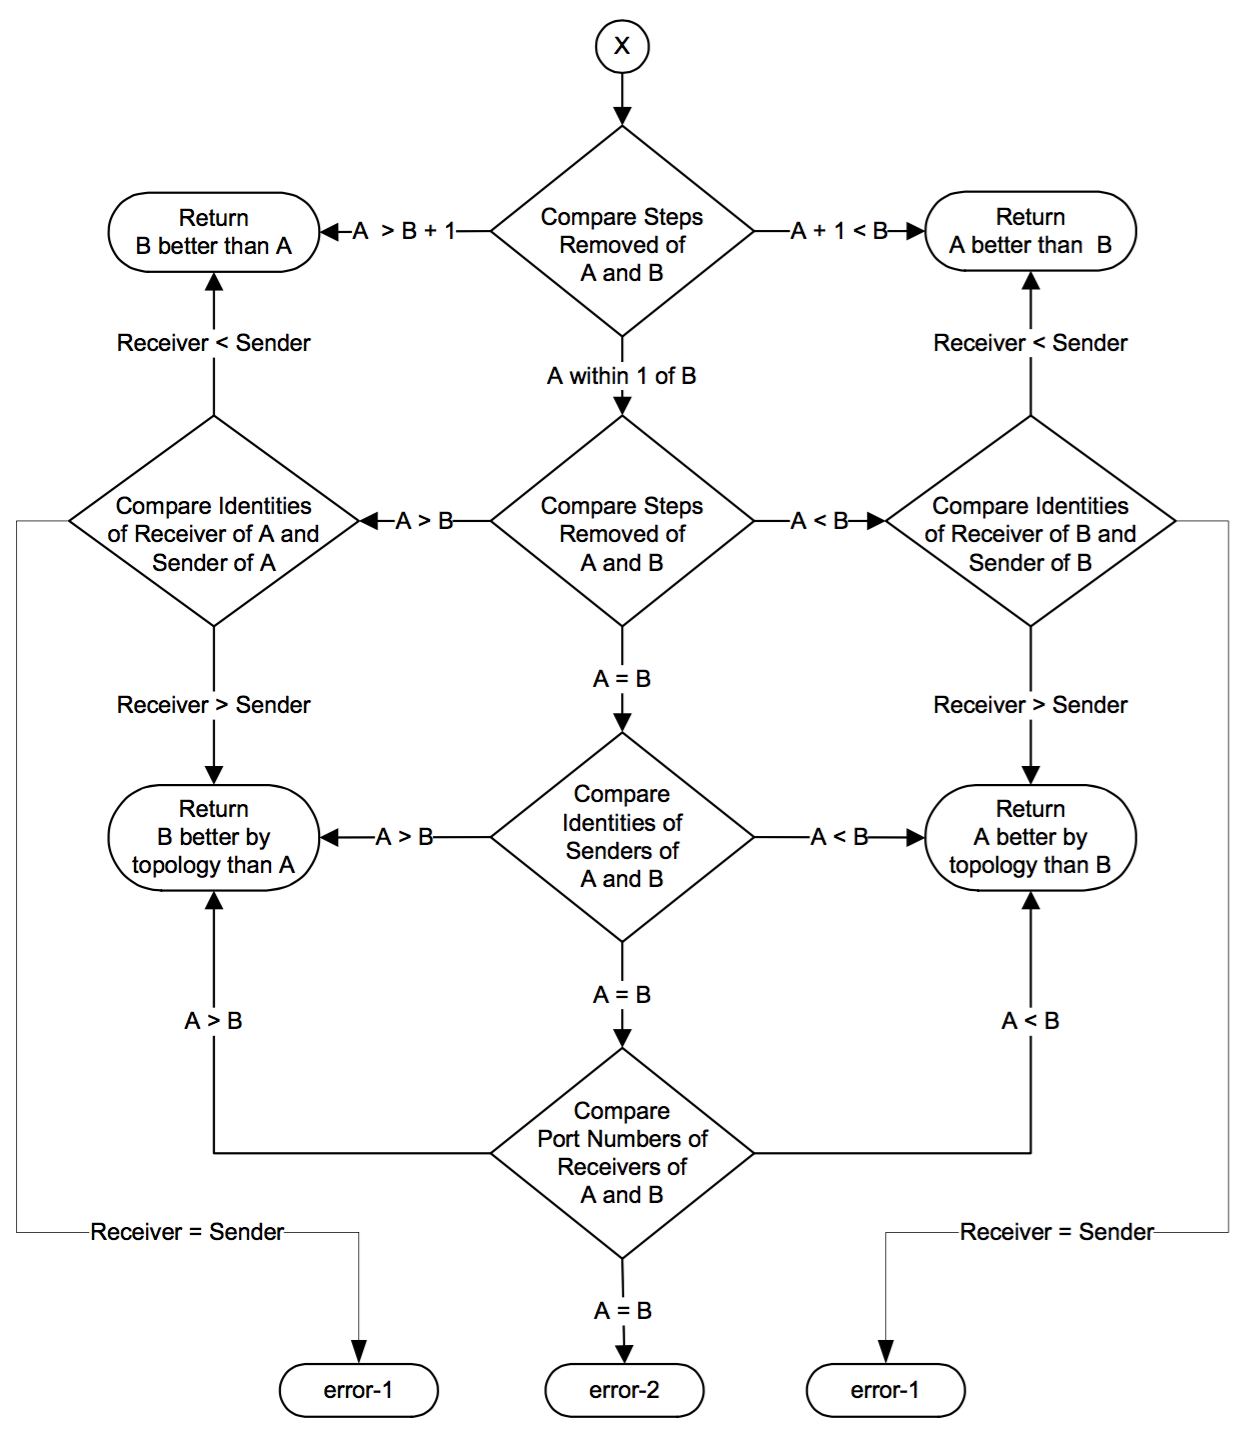
\includegraphics[width=10cm]{dataset_comparison_2}
    \bicaption[fig:dataset_comparison_2]{数据集比较算法Part2}{数据集比较算法Part2}{Fig}{The Dataset Comparsion algorithm Part 2}
  \end{minipage}     
\end{figure}

\subsubsection{状态决定算法}
从上文中可以知道在建立主从秩序时必须依靠数据集比较算法来计算各端口的主从状态,但是,网络内各时钟状态并非一成不变的。假设增加了新的时钟,或者某从时钟自身的精度提高了,此时便需要重新计算各自的状态,所以需要通过状态决定算法在网络运行过程中实时动态地更新各端口状态。

在状态决定算法中,每个节点具有四种状态:初始状态Init、Pre\_Master、Mater和Slave状态。算法如下:
\begin{enumerate}[noitemsep,topsep=0pt,parsep=0pt,partopsep=0pt]
	\item 假设某一新节点加入同步域中,首先默认进入Init状态,同时会持续监听外界主时钟发布过来的Sync报文,该监听会持续一定时间段;
	\item 若在该时间段结束后仍未收到,则进入Pre\_Master状态,此时该时钟会表现主时钟属性,但不对外发送Sync报文;
	\item Pre\_Master会保持一段时间,该时间段内继续等待外界Sync报文;
	\item 若该等待时间超时仍未收到,则变成Master状态,自身开始对外发布Sync报文;
	\item 在正常运行中,若某主时钟收到了精确度更高的Sync报文,那么就会立即停止自身的Master状态,而且不再对外发布Sync报文;
	\item 相反,如果某个从时钟发现自身时钟性能与精度比当前主时钟更好,那么会将自己状态调整成Master,并开始对外发布Sync报文。
\end{enumerate}

网络内各节点都会据此执行状态决定算法,最终系统内所有时钟都动态地更新各自的状态。

可参考图\ref{fig:state_decision}所示。

\begin{figure}[!hbp]
  \centering
  \begin{minipage}[b]{0.8\textwidth}
    \captionstyle{\centering}
    \centering
    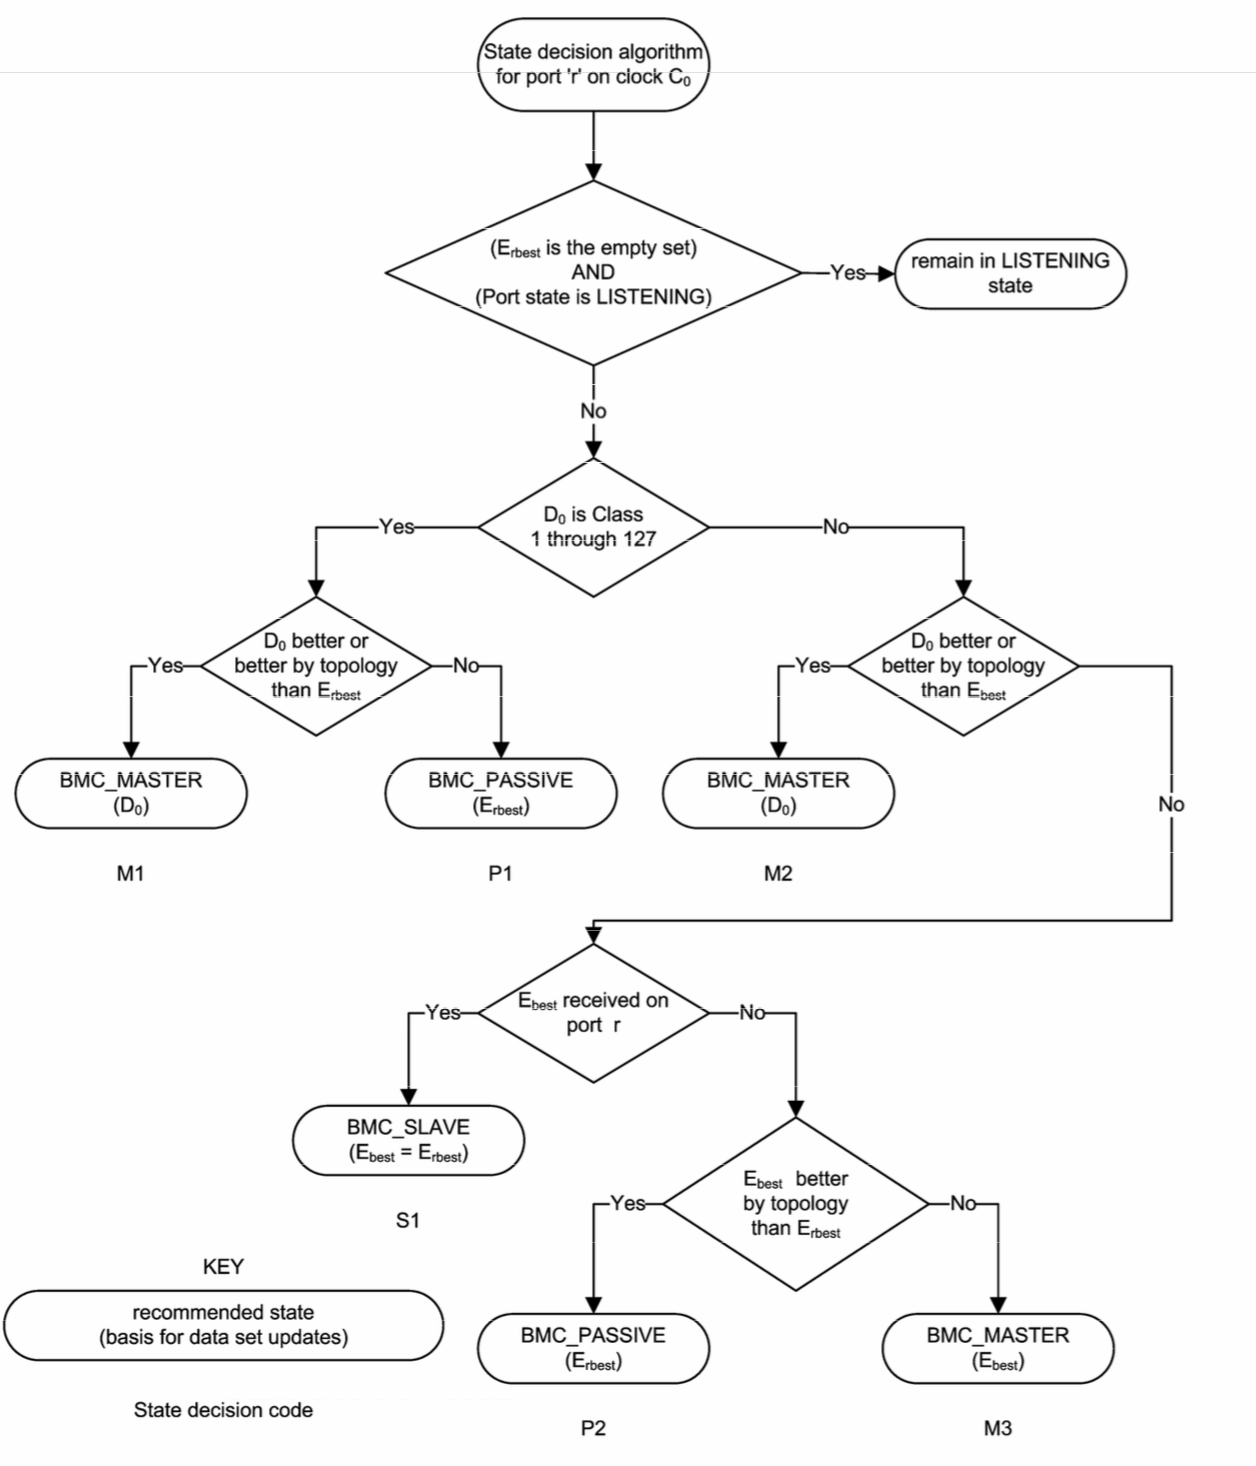
\includegraphics[width=12cm]{state_decision}
    \bicaption[fig:state_decision]{状态决策算法}{状态决策算法}{Fig}{The State Decision Algorithm}
  \end{minipage}     
\end{figure}

\subsection{时钟同步算法}
\label{sec:1588_theory_sync}
在图\ref{fig:process_of_time_sync}中,我们可以看到较为完整的时钟同步过程。下面,对时钟同步过程及相关计算做简明扼要地介绍。

\begin{figure}[!hbp]
  \centering
  \begin{minipage}[b]{0.6\textwidth}
    \captionstyle{\centering}
    \centering
    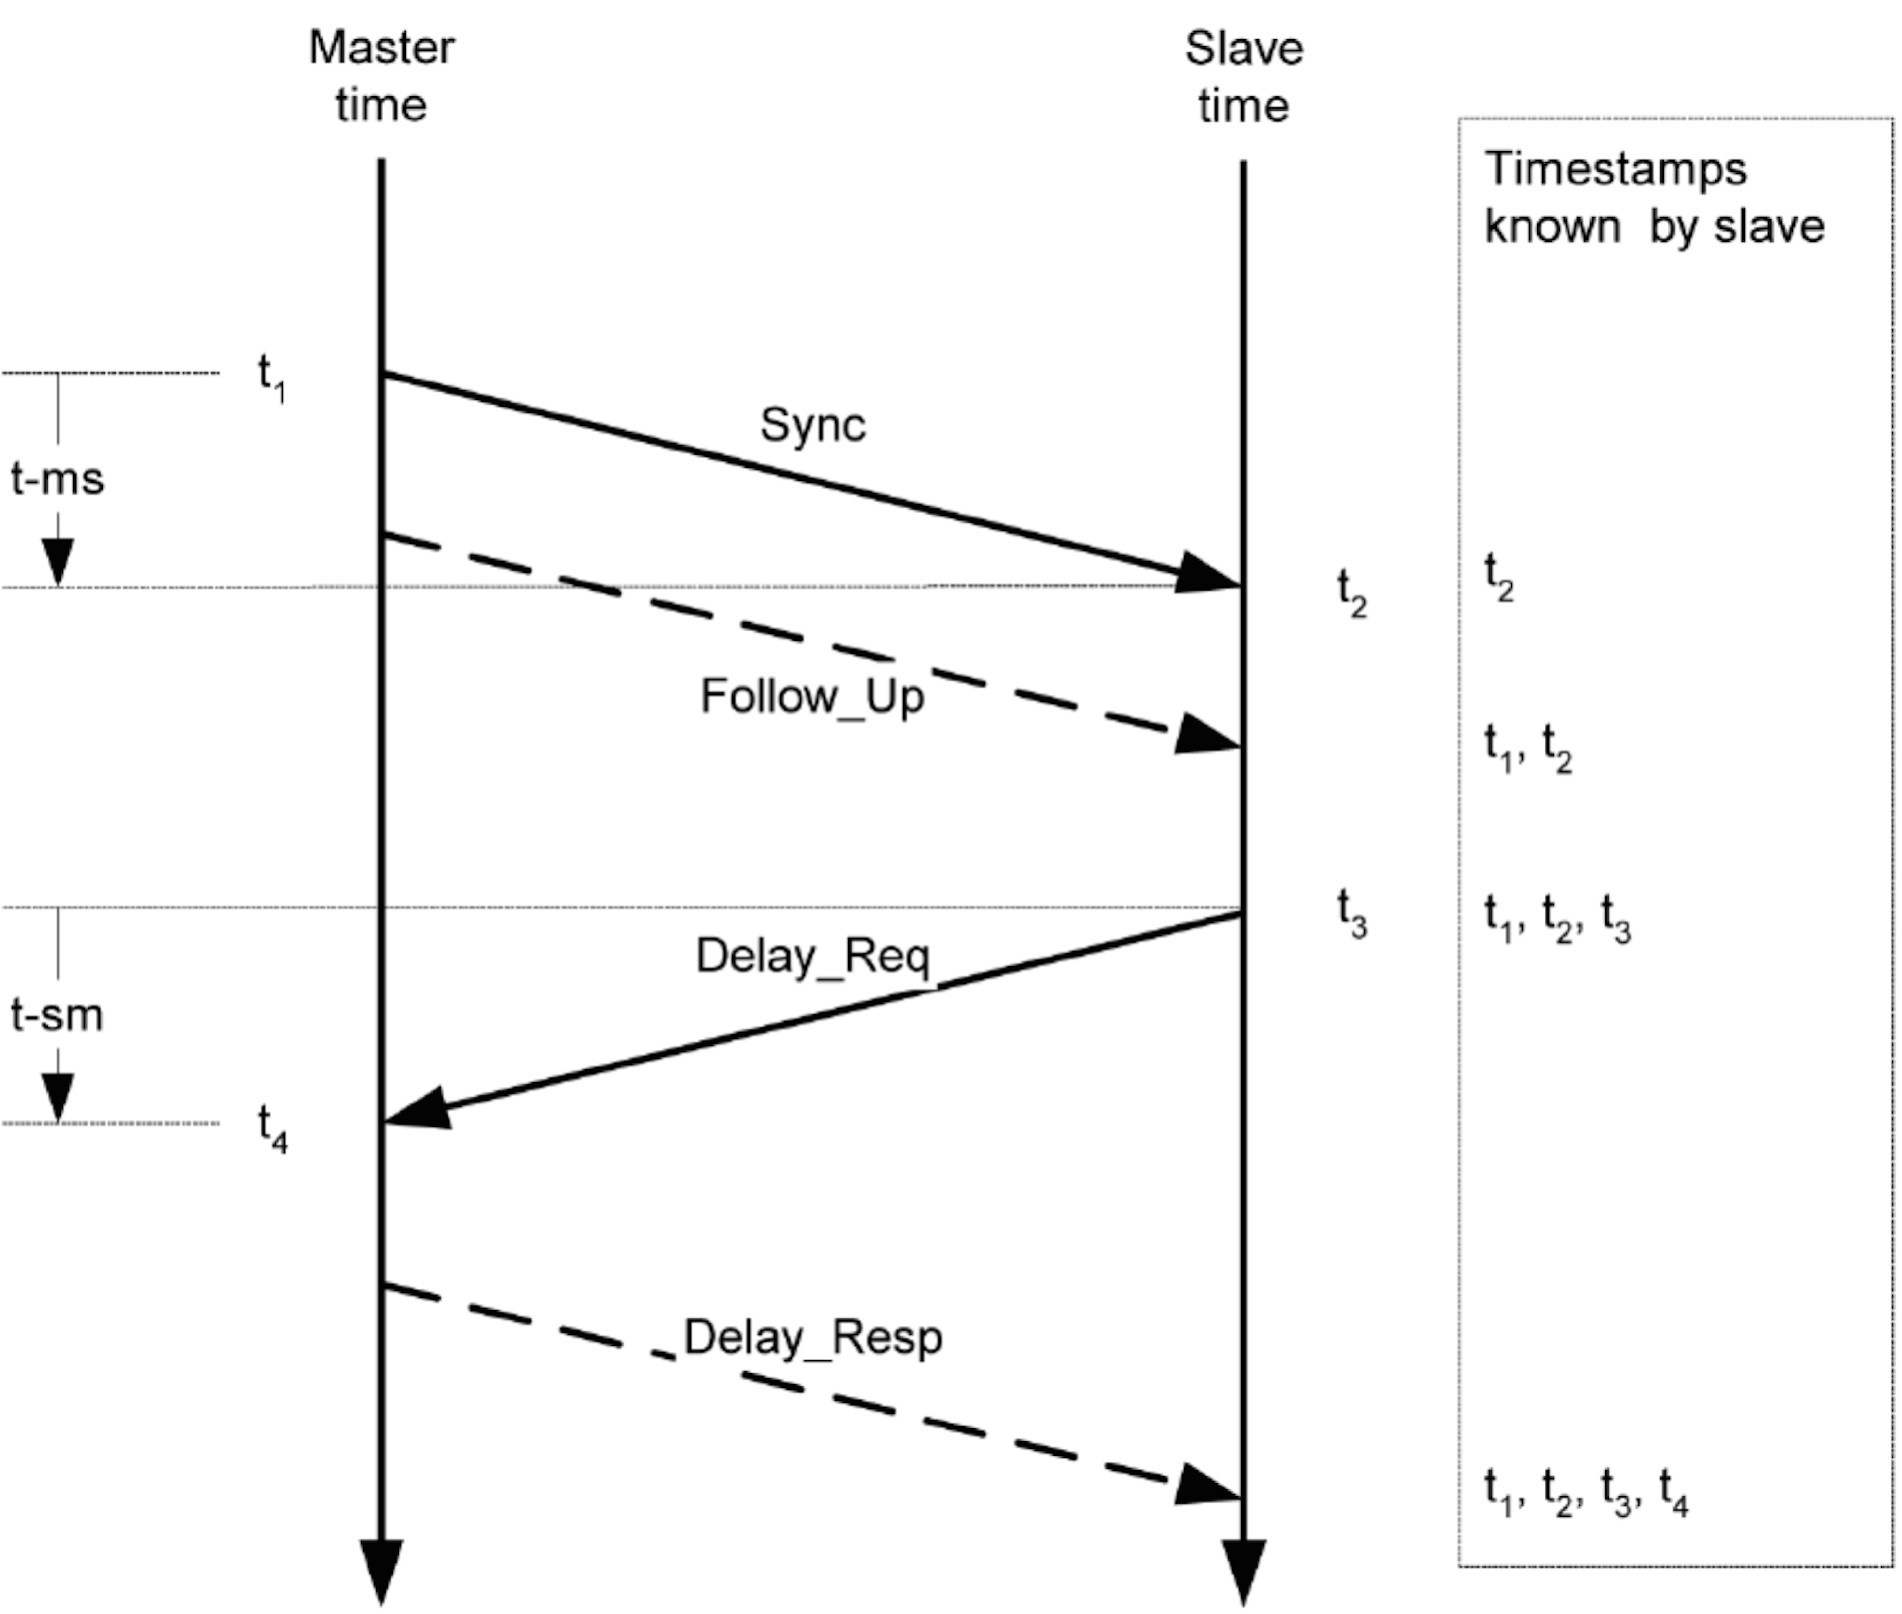
\includegraphics[width=10cm]{process_of_time_sync}
    \bicaption[fig:process_of_time_sync]{时钟同步算法流程图}{时钟同步算法流程图}{Fig}{Method of Time Sync}
  \end{minipage}     
\end{figure}

首先,主时钟会周期性对外发送Sync报文,当该报文离开主时钟时会记录时间戳为t1,若采用硬件时间戳标记的方式则直接把该时间戳存入Sync报文,则无需后续的Follow\_up报文了。

然后,当从时钟接收到Sync报文时,会将接收时间标记为t2。此时,从时钟即获得了Sync报文的发送与接收时间戳t1和t2。那么假设主从时间偏差为$T_{offset}$,主从时钟间网络传输时间为$T_{delay}$,则可以得到下面式子:
\begin{align}
	T_{offset} + T_{delay_1} = t2 - t1
\end{align}

另外,从时钟还会周期性向主时钟发送Delay\_Req报文,假设发送时间为t3,当主时钟收到该报文时,会立即记录下Delay\_Req报文的接收时间t4,并把该接收时间t4存入Delay\_Resp报文中传递回该从时钟。那么此时,从时钟会得到t3和t4两个时间,可得到下面式子:
\begin{align}
	T_{delay_2} - T_{offset} = t4 - t3
\end{align}

此时,我们根据协议标准中,将往返传输延时视为对称,即:
\begin{align}
	T_{delay_1} = T_{delay_2} = T_{delay}
\end{align}
所以,我们结合上面几个式子可以得到如下结果:
\begin{align}
	T_{delay} = \frac{(t2 - t1) + (t4 - t3)}{2}
\end{align}
\begin{align}
	T_{offset} = \frac{(t2 - t1) - (t4 - t3)}{2}
\end{align}

通过上面的计算方法,我们可以得到主从时钟之间的相位偏差$T_{offset}$。然后,我们还需要计算主从时钟的时钟频率偏差才能实现完整的时钟同步。

为了计算时钟频率偏差,我们可以采用下面的方法来计算。我们知道,主时钟是隔固定的周期相从时钟发送Sync报文的,所以,对主时钟而言,第i个Sync报文和第(i+1)个Sync报文之间的发送间隔为:
\begin{align}
	\Delta _{master} = T_{m}(k + 1) + T_{delay}(k + 1) - (T_{m}k - T_{delay}k)
\end{align}
对于从时钟而言,两个Sync报文的时间间隔为:
\begin{align}
	\Delta _{slave} = T_{s}(k + 1) - T_{s}k
\end{align}

所以,我们可以利用上述的比例关系来得到主从时钟的频率偏差。
\begin{align}
	\Delta F = \frac{\Delta _{master}}{\Delta _{slave}}
\end{align}
只需要调节从时钟本地频率扩大$\Delta F$倍就可以实现主从时钟频率一致。

\section{IEEE1588协议实现及分析}
上文中介绍了IEEE1588协议的理论部分,包括主从秩序建立和时钟同步过程。下文会简明扼要地介绍IEEE1588的具体实现过程及相关因素。

\subsection{PTP设备类型}
IEEE1588系统是由PTP设备和非PTP设备结合而成的分布式网络化系统。其中,PTP设备包括普通时钟(Ordinary Clock, OC)、边界时钟(Boundary Clock, BC)、端到端/点到点透明时钟(End-to-End/Peer-to-Peer Transparent Clock, TC)和管理节点。非PTP设备包括普通交换机、路由器及其他底层设备等。

下面对PTP设备作简要介绍:
\begin{itemize}[noitemsep,topsep=0pt,parsep=0pt,partopsep=0pt]
	\item 普通时钟(Ordinary Clock, OC):普通时钟只有一个物理PTP端口,内部包含两个逻辑接口:事件接口主要用来收发含有时间戳的事件报文;通用接口主要用来收发不含时间戳的通用报文。普通时钟指网络中的一般节点,比如电信网基站,或者工业中的测量仪器。
	\item 边界时钟(Boundary Clock, BC):边界时钟包含一个或多个PTP端口,在物理上将一个同步网络划分为多个子网。其每一个端口相当于一个普通时钟,能够引出一条PTP路径,若该端口连接主时钟,则表现从时钟属性;若连接从时钟,则该端口表现主时钟属性。另外,非PTP报文可以通过它来转发,但PTP报文不可以跨越边界时钟。在实际应用中,边界时钟一般安装在路由器、交换机等具有数据收发功能的网络设备上。
	\item 透明时钟(Transparent Clock, TC):透明时钟可以记录报文的进入时间戳和离开时间戳,利用两个时间戳相减得到的相对时间作为驻留时间传递给从时钟,从时钟可以减去该时间从而仿佛报文从未经过该透明时钟,使得波动因素更小。
	\item 管理节点(Management Node):管理节点不需要实现时钟同步功能,它只需要能够对时钟同步进行管理。
\end{itemize}

\subsection{PTP时钟端口状态及状态机原理}
对于一个ptp时钟设备,一般而言它会包含一个或多个端口,每个端口具备自己的状态且相互独立,它们各自的状态都由时钟自身的协议引擎来计算并赋予给它们,而且,处于不同状态的端口对外会有不同表现。

端口状态主要包括以下九种:
\begin{itemize}[noitemsep,topsep=0pt,parsep=0pt,partopsep=0pt]
	\item Initializing:初始化状态。在时钟启动时,端口会进入该状态,此时会完成端口数据集、硬件等多种初始过过程。
	\item Listening:监听状态。该状态表示端口正在监听来自主时钟的Announce报文,而且该状态会有超时时间,即如果在固定时间内仍未收到Announce报文则发生超时。此时会根据状态机规则进入其他状态。
	\item Disabled:禁止状态。若端口处于该状态,则不会对外发送任何ptp报文。
	\item Faulty:故障状态。该状态表明端口故障,不会影响其他端口正常运行。
	\item Uncalibrated:这种状态表明该时钟的所有端口检测到了一个或多个外界主时钟,而且已经从其他端口处选择了主时钟,如果当前端口也检测到了主时钟,为了不发生多个主时钟的问题,当前端口会进入该状态。
	\item Master:作为主时钟,对外界发送同步报文。
	\item Pre\_Master:即刚进入时钟同步系统且未收到任何主时钟的报文,那么会暂时进入该状态,但是此时并不会对外发送同步报文。
	\item Slave:从状态,接受外界主时钟的同步报文并对本地时钟进行同步。
	\item Passive:被动状态。
\end{itemize}

% 下图\ref{fig:port_state_flow}为时钟端口状态机,每个端口的状态变化都会依据该状态机规则进行。

% \begin{figure}[!hbp]
%   \centering
%   \begin{minipage}[b]{0.6\textwidth}
%     \captionstyle{\centering}
%     \centering
%     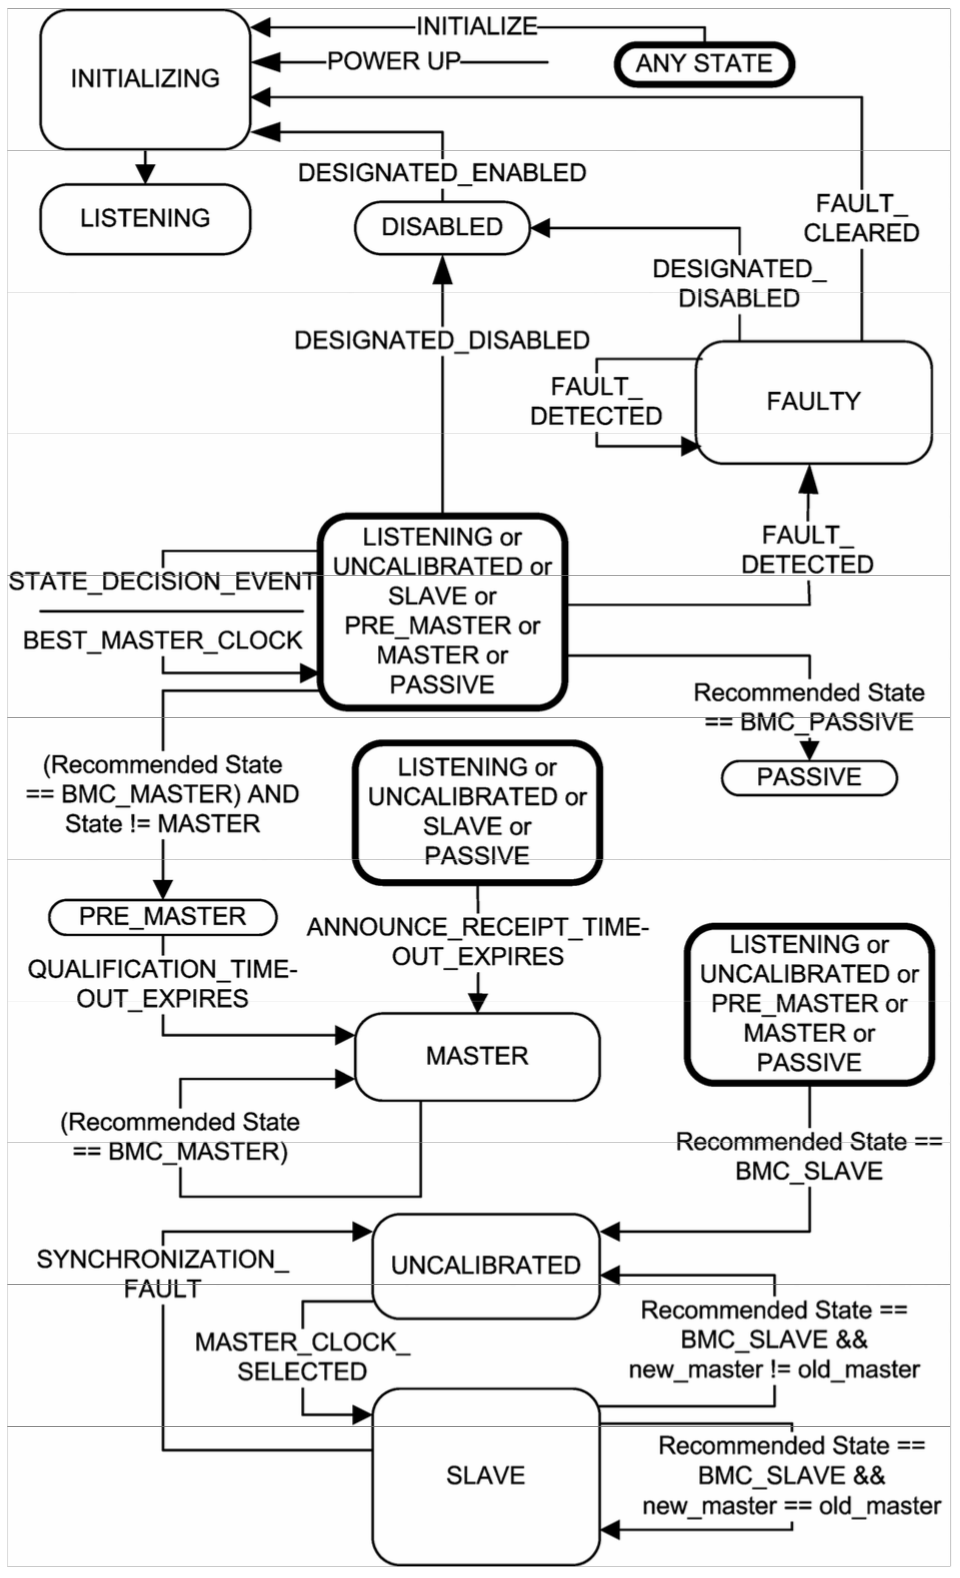
\includegraphics[width=10cm]{port_state_flow}
%     \bicaption[fig:port_state_flow]{端口状态机}{端口状态机}{Fig}{PTP posrState machines}
%   \end{minipage}     
% \end{figure}

下面,将状态机中比较重要的状态转换事件做简要介绍,不作深入研究。
\begin{itemize}[noitemsep,topsep=0pt,parsep=0pt,partopsep=0pt]
	\item POWERUP事件:表示节点上电或者复位。
	\item INITIALIZE事件:表示端口收到了INITIALIZE管理报文等。
	\item FAULT\_DETECTED事件:表示程序在运行过程中,用来阻止协议正确运行的事件。
	\item STATE\_DECISION\_EVENT事件:状态决定事件,即当端口收到有效的Announce报文时会触发该事件,此时将调用BMC最佳主时钟算法来决定各个端口应该进入的状态。
	\item QUALIFICATION\_TIMEOUT\_EXPORES事件:表示端口维持在Pre\_Master状态的时间间隔,其中,qualificationTimeoutInterval一般是Announce报文发送周期的整数倍。
	\item ANNOUNCE\_RECEIPT\_TIMEOUT\_EXPIRES事件:该事件表示端口在规定时间内没有收到Announce报文,即发生超时事件。
\end{itemize}

\subsection{PTP报文介绍}
\subsubsection{PTP报文类型}
PTP协议中的报文分两类,事件(Event)报文和一般(General)报文。下面简单介绍本文使用最多的几种报文。
\begin{itemize}[noitemsep,topsep=0pt,parsep=0pt,partopsep=0pt]
	\item Announce报文:该报文主要用于最佳主时钟算法,报文内部包含描述主时钟所需的数据集,当时钟接收到该报文时,即会调用最佳主时钟算法,比较自身与外部时钟的品质,并根据结果来决定端口的主从状态\supercite{52}。
	\item Sync报文:主时钟周期性对外发送Sync报文,该报文包含了主时钟发送时的时间戳。当从时钟接收到该报文,就会通过offset计算方法来计算出主从时间偏差,并以此来校正自身从而实现同步\supercite{52}。
	\item Delay\_Req和Delay\_Res报文:为了获得主从时钟间的路径传输延时,从时钟会周期性对主时钟发送Delay\_Req报文,当主时钟接收到该报文时,会立即保存接收时间戳,并通过回传Delay\_Res报文把接收时间戳返回给从时钟,用于从时钟的delay值更新\supercite{52}。
\end{itemize}
上面几种报文是本文使用最多的,因此进行了着重介绍。除了上述报文,还有Follow\_Up、PDelay\_Req、PDelay\_Res等报文也非常重要,在此不作过多赘述。

\subsubsection{PTP报文头部格式}
下面分报文头部和报文主体格式进行简单介绍。
所有PTP报文头格式一致,如下图\ref{fig:ptp_message_header}。
其中,各字段含义如下:
\begin{itemize}[noitemsep,topsep=0pt,parsep=0pt,partopsep=0pt]
	\item transportSpecific:标记下一层协议类型,用来区分UDP/IPv6、UDP/IPv4和IEEE802.3;
	\item messageType:标记当前PTP报文类型,包括Sync、Delay\_Req、Follow\_Up、Delay\_Req等;
	\item versionPTP:标记当前PTP版本;
	\item messageLength:标记PTP报文总长度,包含报文头部、报文主体及报文扩展字段;
	\item domainNumber:标记PTP发送端口所属域编号;
	\item flagField:标记单步或双步模式;
	\item correctionField:标记时间修正域,即报文转发时的驻留时间或链路传输延时,该字段为64位有符号整型,意味着它可以使得时间同步精度达到1ns;
	\item sourcePortIdentity:标记发送报文的源端口号,由设备ID及端口ID组成。
\end{itemize}

\begin{figure}[!hbp]
  \centering
  \begin{minipage}[b]{0.6\textwidth}
    \captionstyle{\centering}
    \centering
    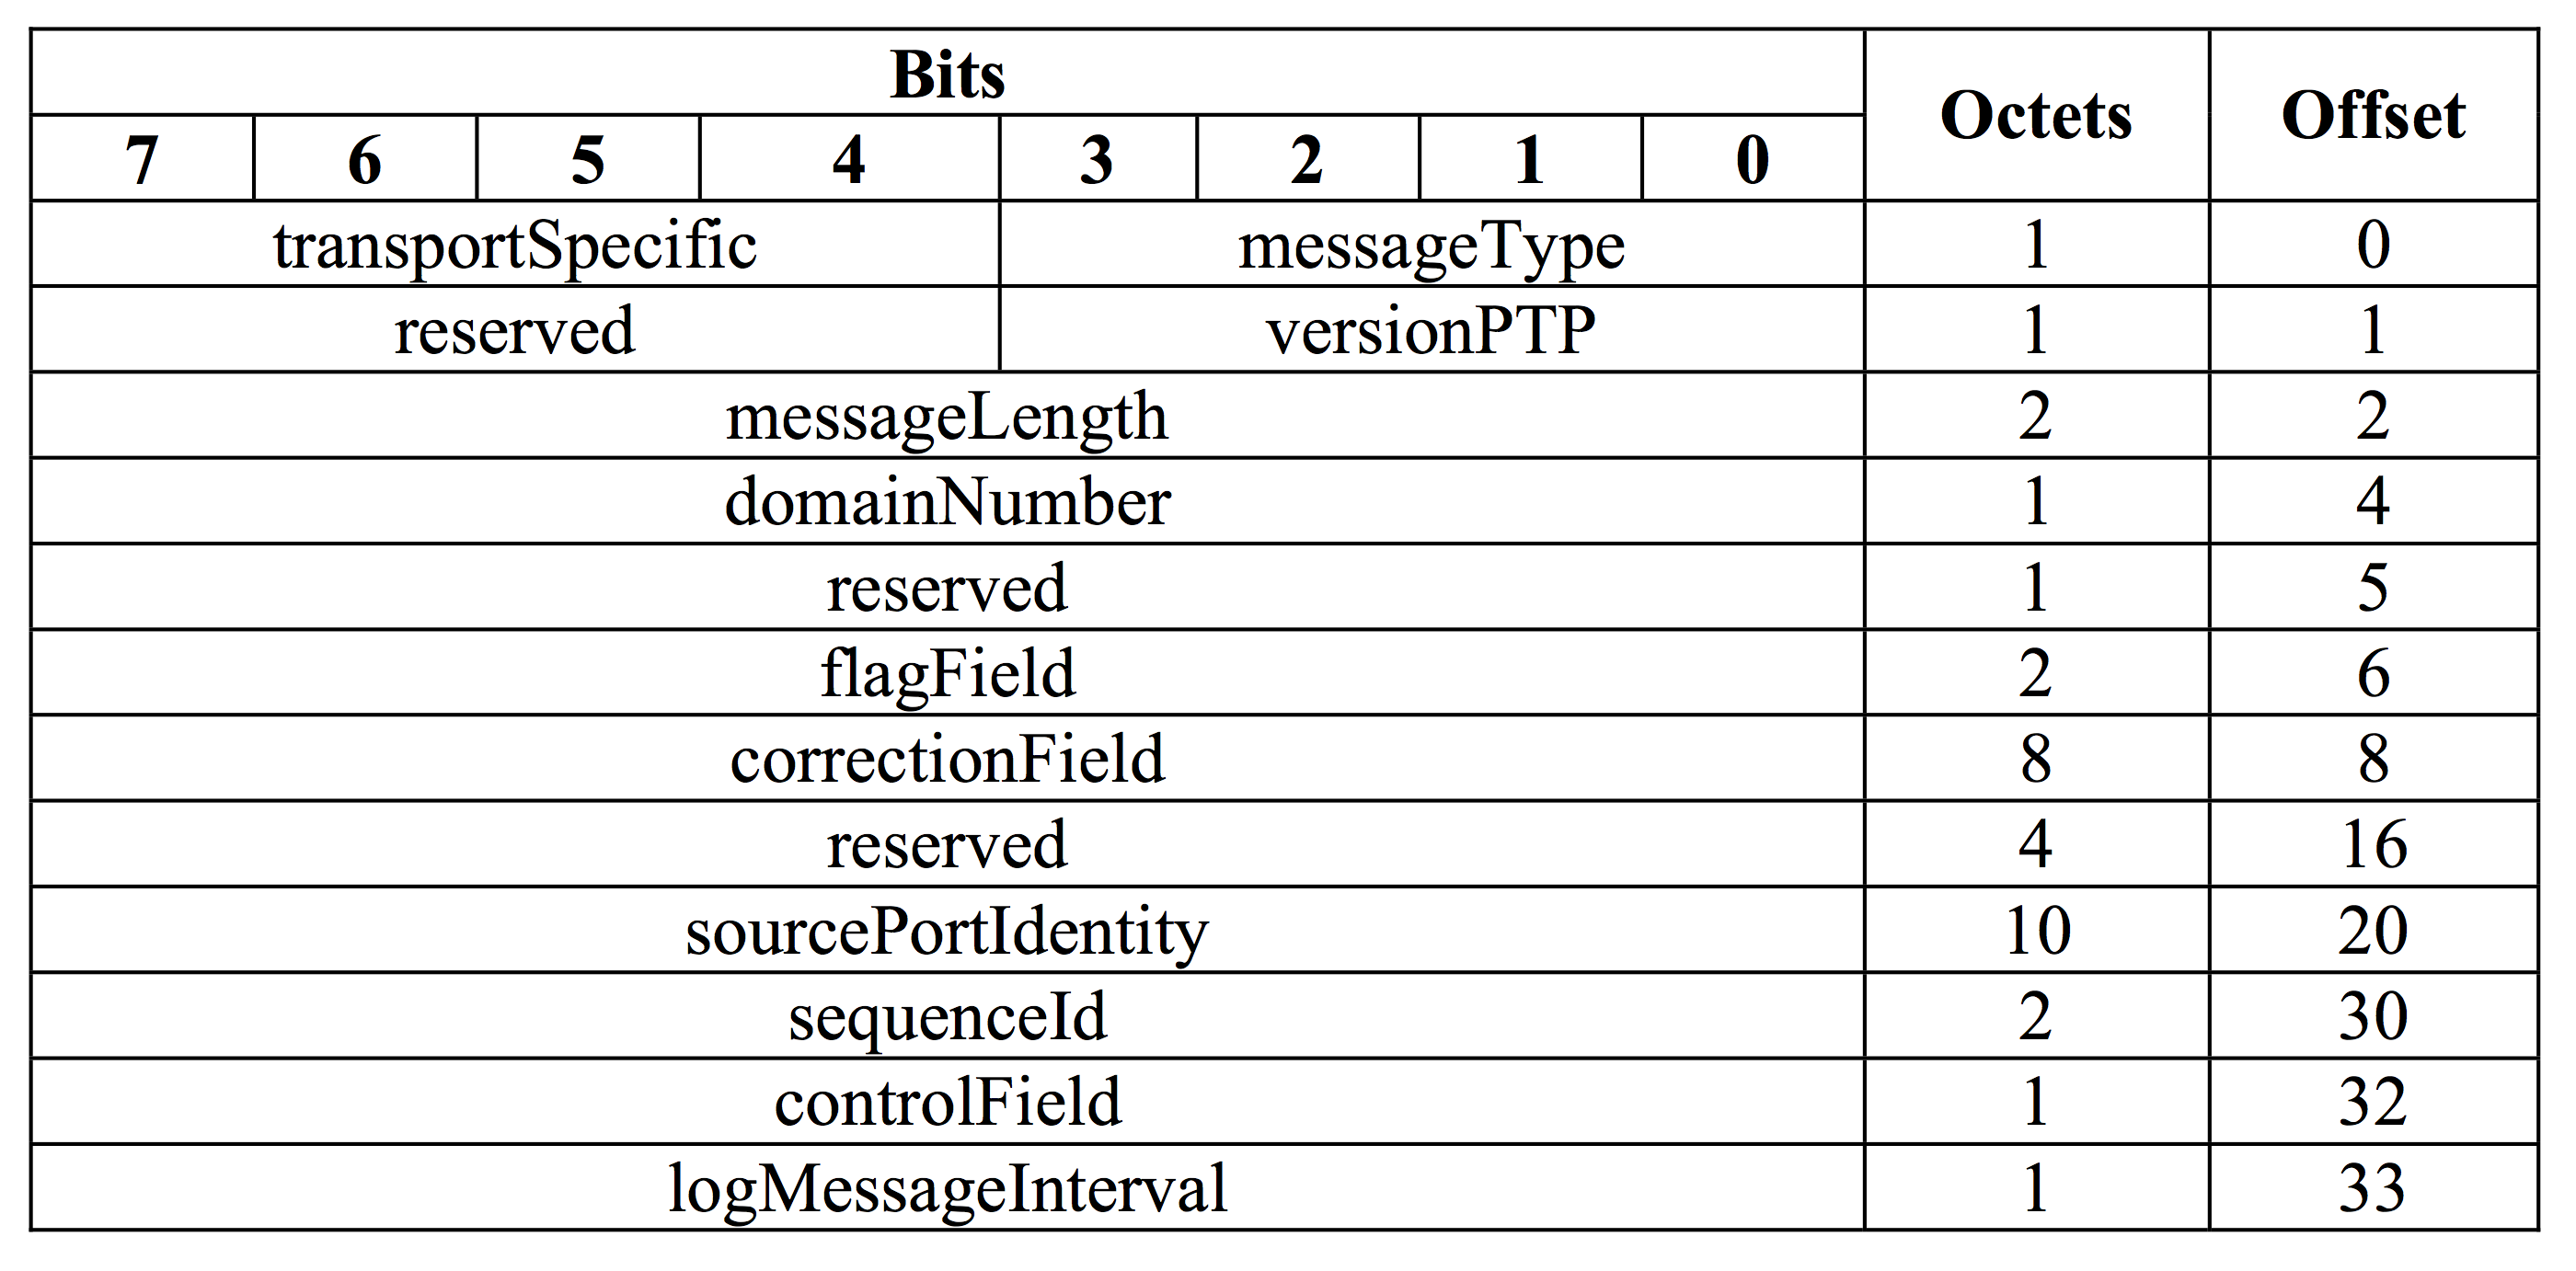
\includegraphics[width=10cm]{ptp_message_header}
    \bicaption[fig:ptp_message_header]{PTP报文头部格式}{PTP报文头部格式}{Fig}{The Style of PTP message Header}
  \end{minipage}     
\end{figure}

\subsubsection{PTP报文主体格式}
PTP报文中的Sync和Req\_Delay两种报文主体主要包括了时间戳信息:NanosecondsField和SecondsField,分别表示时间戳的秒部分和纳秒部分。
\begin{figure}[!hbp]
  \centering
  \begin{minipage}[b]{0.6\textwidth}
    \captionstyle{\centering}
    \centering
    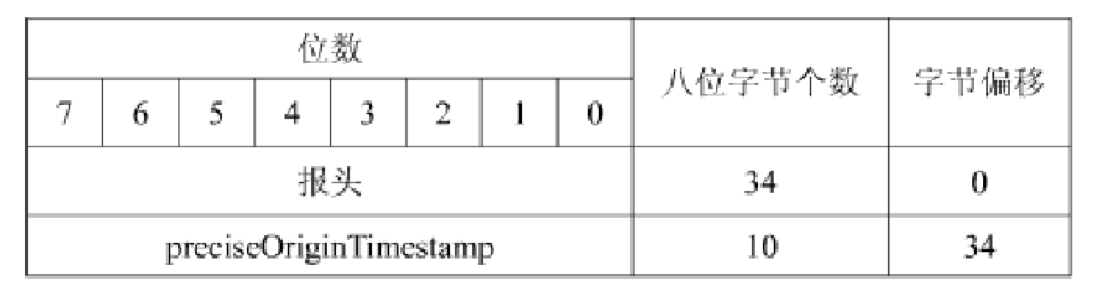
\includegraphics[width=10cm]{ptp_message_content}
    \bicaption[fig:longcaptiongood]{PTP报文主体格式}{PTP报文主体格式}{Fig}{The Structure of Sync Req\_Delay message content}
  \end{minipage}     
\end{figure}

另外,对于Announce报文,其主体内容如图\ref{fig:ptp_announce_message_content}所示:

\begin{figure}[!hbp]
  \centering
  \begin{minipage}[b]{0.6\textwidth}
    \captionstyle{\centering}
    \centering
    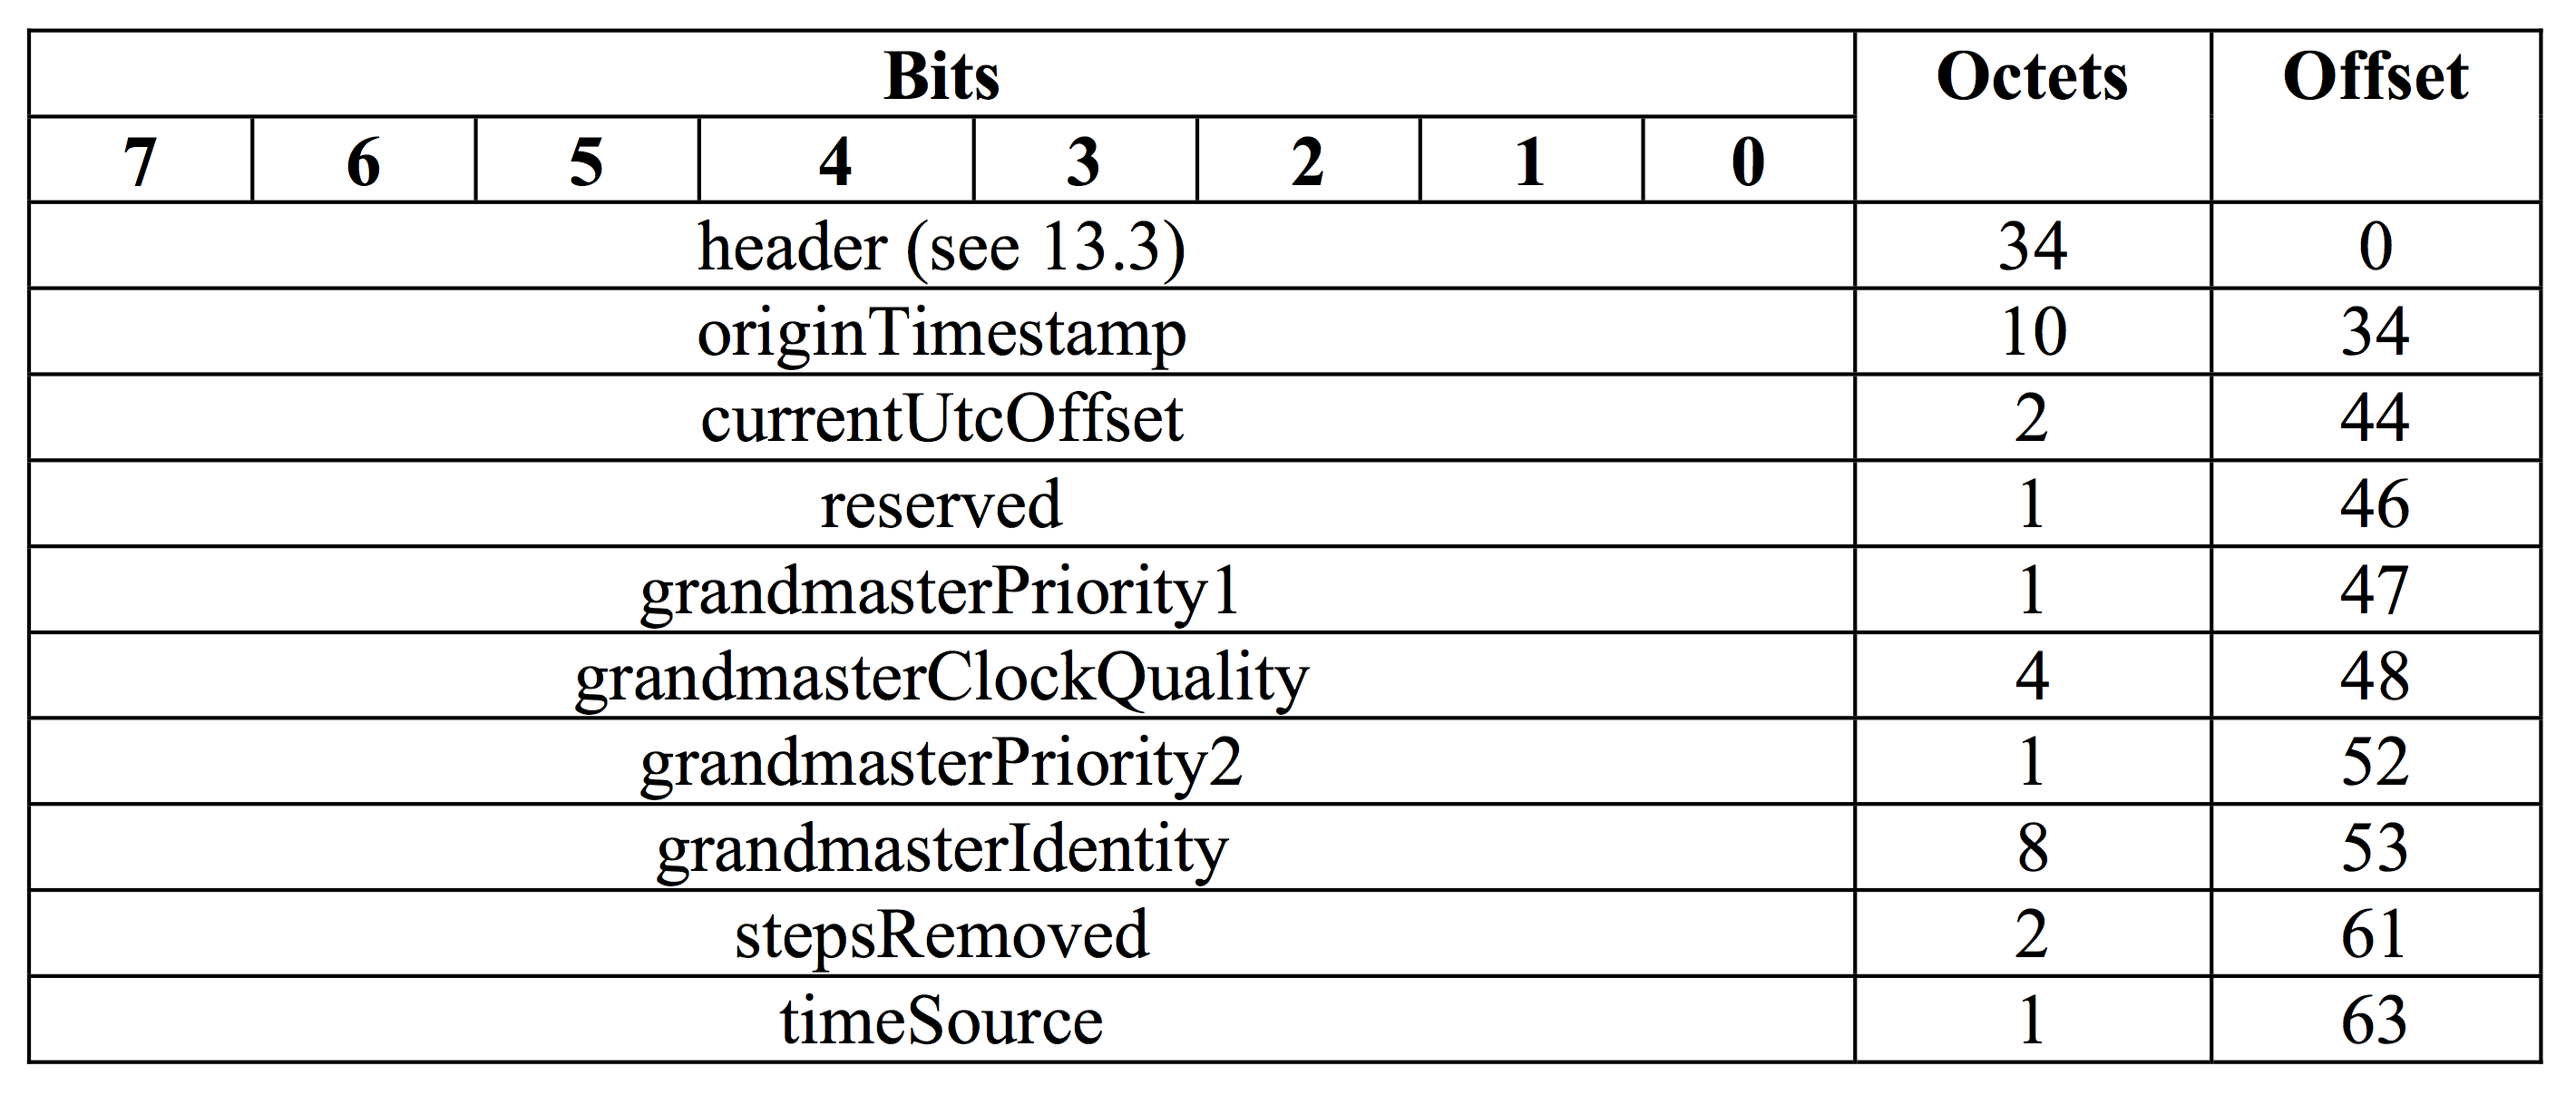
\includegraphics[width=10cm]{ptp_announce_message_content}
    \bicaption[fig:ptp_announce_message_content]{Announce报文主体格式}{Announce报文主体格式}{Fig}{The Structure of Announce message content}
  \end{minipage}     
\end{figure}

其中,grandmasterPriority1、grandmasterClockQuality、grandmasterPriority2和grandmasterIdentity等数据都是用来表示Grand Master的时钟质量,对外发送以让其他时钟能够进行数据集比较算法,然后依靠端口状态变化规则来建立整个系统的主从状态。

\subsection{PTP报文传输周期及其对同步过程的影响分析}
在同步过程中,最重要的便是offset值和delay值的计算,这直接涉及到同步结果的准确性和稳定性;另外还有最初主从秩序建立的快速性也非常重要。所以,下面简单介绍相关的时间周期和超时事件,并分析其对同步过程的影响。
\begin{itemize}[noitemsep,topsep=0pt,parsep=0pt,partopsep=0pt]
	\item Announce报文周期:在实际应用中,该周期值保存在portDS.logAnnounceInterval里,所表示的实际周期为$2^{portDS.logAnnounceInterval}$。协议中规定Announce报文默认发送间隔为2s,可配置范围为1s-16s,采用多播方式。当从时钟接收到该报文,若端口为Slave状态,则会更新本地数据集。
	\item Sync报文周期:该报文周期值保存在portDS.logSyncInterval中,取值范围为-1-1,对应的实际周期为0.5s-2s。每个Master端口都会持续周期性发送该报文,而每次slave端口收到Sync报文就会触发在本地的同步计算并执行校正。对于该值的选取也应该慎重考虑,如果该周期过大,则会使的从时钟偏离太大而失去同步效果;若该周期太小,则会严重加剧网络流量负载,从时钟处于不断的调整波动之中。
	\item Delay\_Req报文周期:该报文周期值保存在portDS.logMinDelayReqInterval中,取值范围为0-5,对应的实际周期为1s-32s,默认值为1s。该报文主要用来更新链路延时delay值。对于该值的选取也应该慎重考虑,如果周期过小,则会给主时钟增加过多的负载压力,加剧网络流量负载;若周期过大,则有可能导致上一次的delay与当前实际delay值出现严重偏差,从而导致offset值偏差较大,严重破坏同步精度。理想的周期应该在区间[0, $2^{portDS.logMinDelayReqInterval+1}$]中均匀分布。
\end{itemize}

\subsection{PTP报文封装传输过程及其对同步精度的影响分析}
首先,一般来讲我们会在应用层准备PTP协议报文,把当前时间戳信息作为传递数据打包进去并传递给传输层;然后,操作系统按照网络协议栈将应用层数据依次打包进入UDP传输层报文和IP网络层报文;然后从网络层发送给数据链路层,该层会为报文添加以太网帧的首部和尾部形成完整的以太网报文,发送给物理层硬件发送出去\supercite{54}。

\section{IEEE1588实际应用中存在的问题及本人研究目标}
在上文中,主要介绍了IEEE1588协议的实现原理。根据我们对原理如时钟同步算法的分析研究,再加上PTP协议在工业实际中的精度表现,可以发现该协议中仍然存在一些影响精度的因素,而且,如果我们希望实际精度能够达到微秒级甚至纳秒级,就不得不对这些因素进行深入的研究。下面本人结合IEEE1588的实现原理及实际表现,提出其中存在的固有弊病和漏洞,正是这些问题导致了实际运行中的同步精度难以达到亚微秒级。

\subsection{链路延时不对称}
\label{sec:1588_problem_1}
在IEEE1588协议中,当计算主从时钟偏差offset时,需要先获取链路传输延时delay。在协议中该延时的计算方法是直接假设前后两次传输延时相等,从而通过取平均计算出offset。然而实际上,前后两次的传输路径往往并不对称,经过分析,可以发现以下几个导致往返的链路传输延时不一致的因素\supercite{55}。
\begin{itemize}[noitemsep,topsep=0pt,parsep=0pt,partopsep=0pt]
	\item 排队堵塞:当报文在传输中经过中间交换机或路由器时,由于网络负载的不可预知性,我们无法知道报文在中间交换机上的排队时间,当网络流量良好时,报文可以直接传递过去;而当网络负载较大,可能导致很长的报文排队时间。另外,即使报文可以不用排队,由于协议栈的存在,报文仍然需要经过解包和打包的过程,而这两个过程的消耗时间都与操作系统的调度和协议栈处理过程有关。因此,报文传递过程中穿越交换机时排队和堵塞时间的随机性会导致延时不对称\supercite{46}。
	\item 传输抖动:在网络系统中,所有信息的传递过程所消耗的时间会存在固有的抖动,这时无法避免的。
	\item 网络拓扑结构变化:当拓扑结构突然发生变化,报文传输的路径也就不同了,这必然导致往返链路时延完全不同。
	\item delay与当前真实延时不匹配:因为delay的计算依靠Delay\_Req报文周期,而offset的计算又是依靠Sync报文周期,两者一般并不匹配。所以会导致在计算offset所使用的delay是过去的值,与当前真实的delay值可能并不一致。
\end{itemize}

上述几种现象的存在,都会导致往返的两次延时不一致,所以说,在高同步精度的要求下,真实的传输延时绝对不能简单的假设相等。

对于网络延时的研究,也正是本文的重点内容。本人在接下来的内容中,会对上述所提到的几种因素进行拆解分析,同时,从数学统计的角度,把所有历史延时数据作为样本,采用多个统计方法来对数据进行处理和消除干扰,从而得到稳定的同步数据。

\subsection{时间戳的精确度}
\label{sec:1588_problem_2}
在上文中的报文的封装传输过程已经提到,由于在协议栈中传递所带来的延时,导致物理层之上的时间戳往往不能真实反映报文的发送时间或接收时间,若直接使用这种时间戳来进行计算,那么从根本上就带来了误差\supercite{53}。所以,如果一些设备采用的是软件时间戳方式,那么报文的封装和解包过程就势必会对真实的时间戳产生偏差,这种时间戳精确度上所带来的误差是不可忽视的。

不过,在本人所参与的交换机项目中,我们采用的是支持硬件时间戳的设备,该设备能够直接在数据链路层与物理层之间为报文添加时间戳,从而保证了时间戳的精确度,因此,在本文中,并不会对该因素作过多深入的探讨和研究。

\subsection{从时钟稳定性}
\label{sec:1588_problem_3}
根据IEEE1588协议,当从时钟收到Sync报文,便立即进行offset值的计算。当得到offset值,即主从时钟偏差后,便会对从时钟相位直接进行校正。这种校正策略有很好的快速性,使的从时钟在很短的时间内实现与主时钟同步。但缺陷是,这种做法并没有考虑到offset值的准确度,如果由于延时的存在导致offset值出现较大的偏差,那么从时钟则会一直处于快速的振荡状态,这对于从时钟系统而言是非常不利的。

为了兼顾从时钟的同步快速性和自身稳定性,本人在接下来的内容中,会从下面三种从时钟控制策略入手,通过分析并仿真实践来进行对比。
\begin{itemize}[noitemsep,topsep=0pt,parsep=0pt,partopsep=0pt]
	\item 直接校正;
	\item 常规PI控制器校正;
	\item 基于BP神经网络的PID控制器校正。
\end{itemize}





%# -*- coding: utf-8-unix -*-
%%==================================================
%% chapter_3.tex for SJTU Master Thesis
%%==================================================

\chapter{基于统计的链路延时误差优化方法}
\label{chap:statistical_delay}
本章在分析链路延时实际影响因素的基础上,针对链路延时建立了较为完整的数学模型,然后通过对该模型的统计特性进行分析,结合从时钟的时延历史样本,文中将依据统计方法来研究对真实链路延时的估计算法。

\section{链路延时不对称性的影响因素}
在实际的工业现场中,由于如延时固有抖动、报文的堵塞等多种因素,都会导致往返的链路并不对称。因此为了达到亚微秒级别的同步精度,文章将对链路延时进行深入探究,主要包括以下几个因素。

\subsection{网络传输抖动}
在网络系统中,所有信息的传递过程所消耗的时间会存在固有的抖动,这是无法避免的,也是引起链路延时不对称性的主要原因。
通常认为网络流量随机过程符合马尔可夫模型或者泊松分布。其中,马尔可夫模型表示对历史具有有限的记忆,或者说在已经知道现在的前提下,其将来并不依赖于过去;而泊松过程中的随机变量(单位时间呼叫达到的次数)是独立且服从自相似分布的\supercite{12}:
\begin {align}
P(X_{k} = n) = \frac{n\lambda\Delta t e^{- \lambda\Delta t}}{n!},n\geq 0;
\end{align}
通过试验测量分析认为,网络流量序列在很宽的时间尺度内存在突发现象,或者说,Internet网络流量序列符合自相似特性\supercite{13,14,15,16},即样本均值的方差比样本个数的倒数减小得更慢。另外,文献\parencite{17}对于NTP时间包全程延时作了大量研究,文献\parencite{18}利用两主机之间通过传送带时间标签的UDP包测量全程延时,得到了相同的结论,即认为Internet网络流量及延时具有一定随机抖动。而以太网是构成Internet网的主要部分,所以有理由认为以太网网络流量及延时也具备随机抖动。

\subsection{网络拓扑结构变化}
一般的PTP同步系统拓扑结构如图\ref{fig:1588_sync_topology}所示:
\begin{figure}[htbp]
  \centering
  \begin{minipage}[b]{0.6\textwidth}
    \captionstyle{\centering}
    \centering
    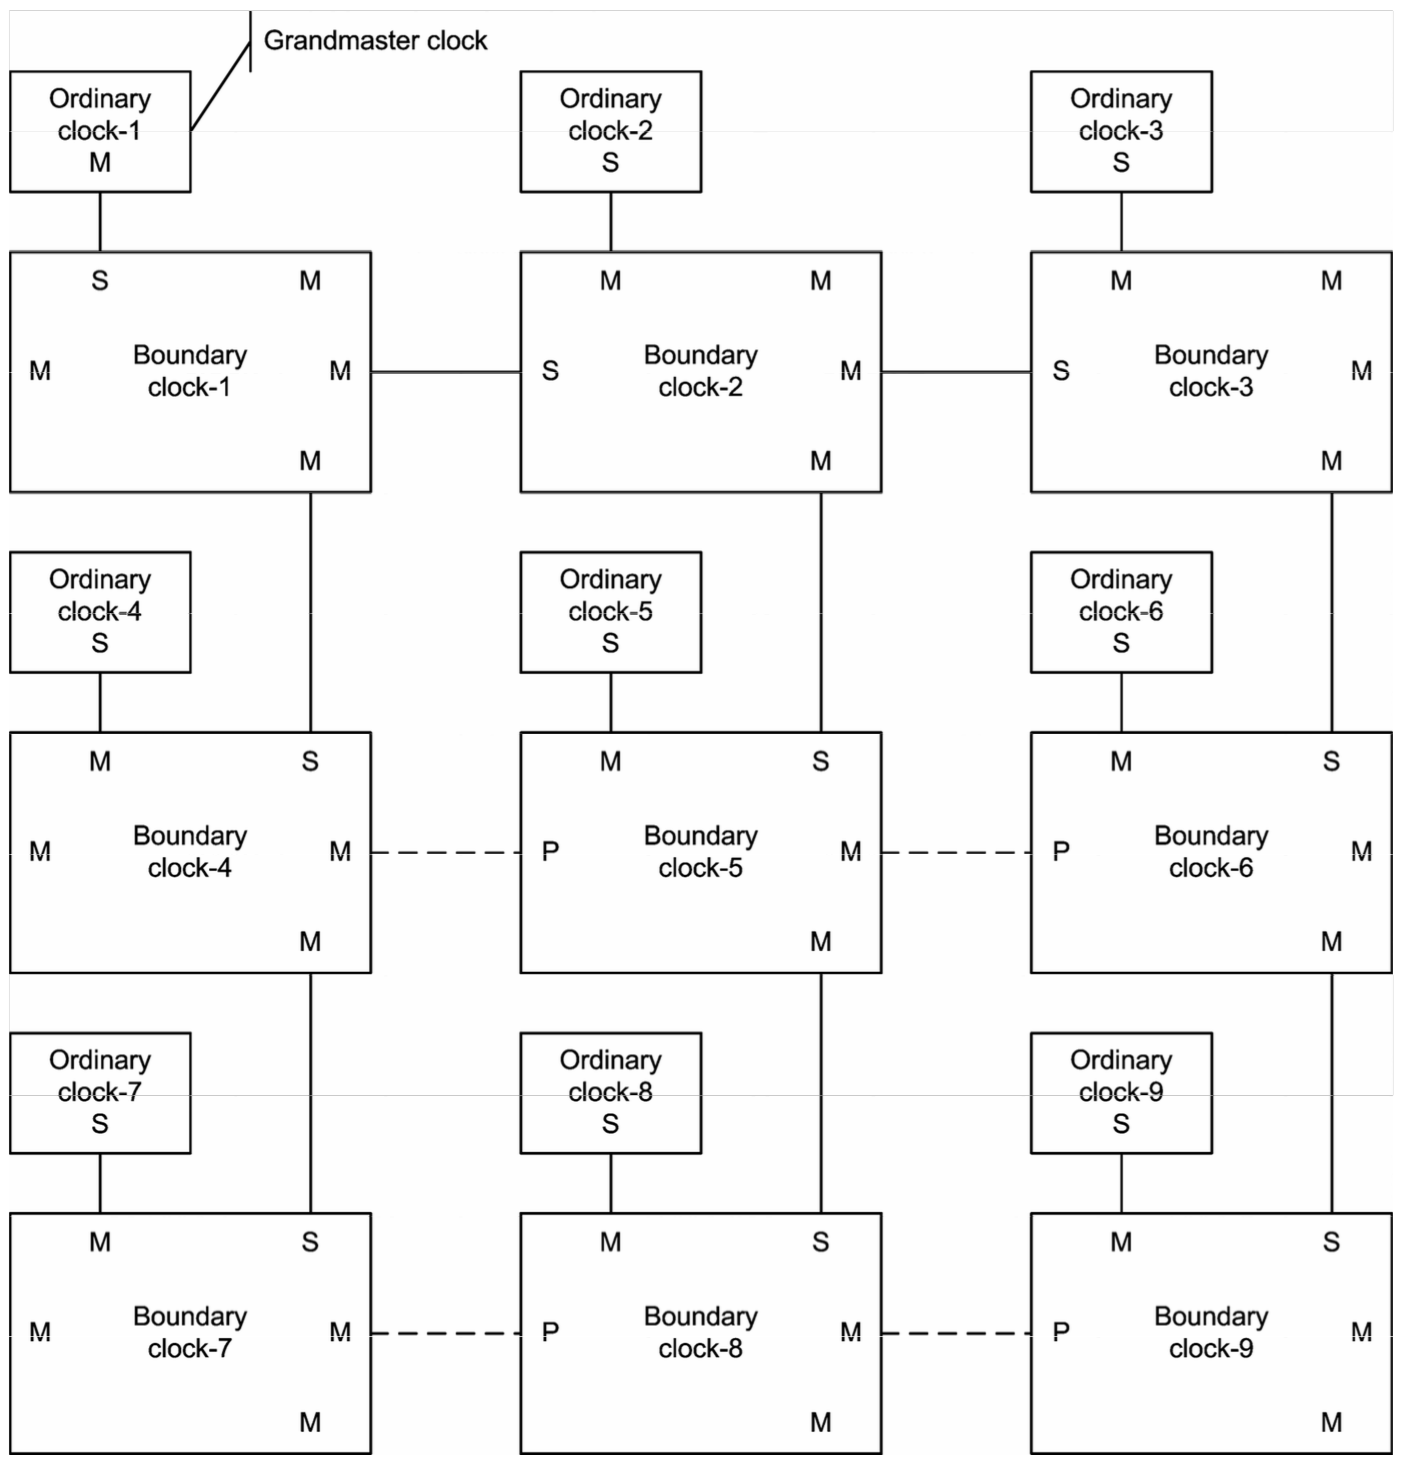
\includegraphics[width=10cm]{1588_sync_topology}
    \bicaption[fig:1588_sync_topology]{分布式同步系统结构图\supercite{2}}{分布式同步系统结构图\supercite{2}}{Fig}{The Structure of distributed sync system}
  \end{minipage}     
\end{figure}
\\ \\ \\

假如同步系统中由于环路结构的快速重配置等原因导致链路的拓扑结构发生改变,将导致报文传输的往返延时的不同,而这也导致计算出来的延时值与实际值有很大偏差。然而,在现有的IEEE1588协议中,并没有很好的去探测链路结构的变化并针对性做出处理。这也正是本章节的重点研究内容。

\subsection{$T_{delay}$与当前真实延时不匹配}
因为$T_{delay}$的计算依靠Delay\_Req报文周期,而$T_{offset}$的计算又是依靠Sync报文周期,两者一般并不一致。所以会导致在计算$T_{offset}$所使用的$T_{delay}$是过去的值,与当前真实的$T_{delay}$值可能并不一致。所以,这会导致多数时候计算所使用的$T_{delay}$值并不一定等于真实的$T_{delay}$值,从而出现误差。

% \subsection{报文排队与堵塞}
% 在同步过程中,一般而言,主从时钟之间的报文传递会穿越一些中间设备如交换机或路由器等设备,而这些设备存在的主要作用是转发同步报文。可想而知,一个报文从进入该设备直到离开所消耗的时间必定是链路传输延时的一部分,相比简单的直线线路传输,该中转过程对链路延时变化有着极为重要的影响。下面将报文驻留于中间设备的总驻留时间分解成排队和堵塞两部分介绍。
% \subsubsection{报文排队}
% 当报文进入一个如交换机的中间设备时,它会首先进入报文队列缓冲区,所有外界进入的报文都会首先进入该队列中,然后交换机系统会依次把报文取出处理并继续对外转发。当网络负载情况良好时,交换机会有很快的响应速度,即报文一进入队列缓冲区就可以立即得到转发处理\supercite{46,47}。

\subsection{传输链路堵塞}
在真实的工业网络环境中,网络负载总是在实时变化的。一旦交换机内部负载过大,队列缓冲区堆积了较多的待转发报文时,新进入的同步报文则会保持在队列末尾进行等待,直到交换机把前面的所有报文都转发处理了才轮到该同步报文转发。而在这个等待过程中所消耗的时间完全取决于网络负载情况和交换机内部队列的密度,这种时间对于从时钟而言是完全无法预知的。所以,很有可能前后两次的往返报文在穿越中间某个交换设备时,所消耗的等待时间会有很大差异,而正是这种差异的存在,即报文堵塞时间的不可预知性和随机性,导致了链路延时的不对称性。当报文进入中间交换设备时,会先转发操作。然而,该转发操作并非瞬间完成的。当报文进入交换设备,会依赖于该交换设备的协议栈并得到解包和打包处理。所谓解包即交换设备根据自身协议栈把报文层层解析得到用户数据,打包即重新把用户数据封装并向协议栈底层传递。这个过程称之为堵塞时间,即交换设备空闲,但由于协议栈的存在导致报文必须驻留的解析时间。所以,在报文得到处理到真正离开中间设备,中间必须经过一段堵塞时间。而堵塞过程中的解包和打包操作,均需要操作系统分配CPU来进行处理。而操作系统的调度是完全随机的,无法提前预知操作系统的调度策略,也无法预知该解析过程所真实需要耗费的时间。尽管这些时间非常微小,但对于想要达到亚微秒同步精度的同步系统而言,这样的时间偏差不可忽视。

\section{链路延时数学建模}
如前文所述,报文的传输过程所受到的影响因素主要有以下几点:延时固有抖动会导致延时发生固有的小幅波动;拓扑结构变化或网络重配置将使得链路传输延时与之前的延时会发生明显变化,即新延时不再与旧有延时有任何关系;链路传输堵塞的发生取决于网络状况,网络良好时,该延时时间非常短,但当网络负载加剧,则延时会突然剧烈增大为T1,直到网络恢复,因此可以认为这种情况导致的延时增大往往是暂时性的。基于此,可以用下列数学模型\supercite{33}来进行描述链路传输延时:
\begin {align}
T_{all}(i) = T_{pure}(i) + T_{queue}(i) + T_{jitter}(i)  \qquad i=1,2,3...
\end{align}
其中,i表示同步过程中的第i次报文传输,$T_{all}$代表单次链路传输总延时,$T_{pure}$代表在不考虑任何堵塞和抖动的情况下,在固定传输路径上的延时,$T_{queue}$代表在该次链路传输过程中,发生的堵塞等导致的总延时,$T_{jitter}$表示该次传输中存在的抖动延时。为保持简洁,用下面公式代替:
\begin {align}
T(i) = T_{p}(i) + T_{q}(i) + T_{j}(i)
\end{align}

\subsection{固定拓扑结构下的纯粹链路延时}
对于$T_{p}$,用来表示在固定的拓扑结构下,不考虑堵塞和抖动等外界干扰的纯粹链路延时。容易知道,只要链路保持不变,那么$T_{p}$就不会发生改变,也就是说,假设网络配置情况等保持一定的概率为$P_{path\_stable}$,那么$T_{p}$就为常量,即
\begin {align}
T_{p}(i+1) = T_{p}(i) \qquad probability: P_{path\_stable}
\end{align}
\begin {align}
T_{p}(i+1) \neq T_{p}(i) \qquad probability: (1-P_{path\_stable})
\end{align}
正常来说,网络重配置的概率非常小,也就是说$P_{path\_stable}$值非常小。但是,如果一旦发生了网络重配置,那么未来的延时与过去的延时将很有可能出现很大变化。

基于上述特性,在此将拓扑结构变化延时定义为持久性时延变化。

\subsection{链路传输堵塞}
对于$T_{q}(i)$,用来表示报文在传输过程中经过中间转换设备时的驻留时间。正常情况下,即当网络中流量负载良好时,$T_{q}(i)$会保持一个微小的驻留值,接近为零。但是,一旦网络负载突然加剧,那么$T_{q}(i)$会瞬间增大,而且网络负载越大,则$T_{q}(i)$会有越明显的突变。这直接导致的后果的前后几次测量的$T_{delay}$值有明显变化,从而影响到从时钟的精度。
所以,假设网络流量繁忙的概率为$P_{net\_busy}$,那么可以用如下公式\supercite{33}来描述堵塞延时:
\begin {align}
T_{p}(i) = S(i) \cdot W(i) 
\end{align}
\begin {align}
S(i) = 1 \qquad probability: P_{net\_busy}
\end{align}
其中,$S(i)$是一个开关量,等于1的概率为$P_{net\_busy}$,或者说,当网络繁忙时,$S(i)$便为1;反之,当网络空闲时,$S(i)$便为0,即堵塞延时$T_{q}(i)$也为0。$W(i)$则表示真实的堵塞延时。不过一般而言,网络繁忙持续时间较短,所以在多数时间$T_{q}(i)$取值接近零,偶尔会发生阶跃性突变。

基于上述特性,在此将报文堵塞延时定义为暂时性延时突变。

\subsection{链路传输延时固有抖动}
对于$T_{j}(i)$,用来表示传输延时的固有抖动成分。该抖动主要基于$T_{p}$,度量真实链路传输时间对平均时间的偏差值。从宽时间序列角度来看,对于随机变量$T_{j}(i)$的期望值有如下公式\supercite{33}:
\begin {align}
E\{T_{j}(i)\} = 0
\end {align}
这里,假设$T_{j}(i)$的方差值为$\sigma ^{2}$。$T_{j}(i)$都是独立同分布。

\subsection{链路传输延时模型分析}
上文中已经从数学模型角度,建立了多个方程来描述链路传输延时T。由于本文的根本出发点是利用历史延时数据作为样本来共同估计当前真实延时,即从时钟端会通过收集并保存历史时延样本,然后利用这些历史时延样本数据,采用结合最小二乘法、动态阈值法和滑动固定时间窗实时检测三种方法来共同消除上述因素对延时造成的误差。

下面从历史延时数据样本角度切入,来对上文中所建立传输延时数学模型进行分析并采用相应的解决方法。

\subsubsection{链路传输固有延时$T_{j}(i)$}
由于该固有延时是以太网流量中存在的随机因素,且可以认为$T_{j}(i)$是小幅波动的干扰噪声。这种干扰噪声会导致最终的传输延时处于小幅随机波动中。一般而言,针对此类随机变量最好的处理方法就是依靠历史样本进行滤波,因此,在下文中将采用基于最小二乘法的滤波法,通过对历史延时样本进行线性回归,得到一条直线并以此来估计当前时延,从而滤除此类随机干扰噪声。

\subsubsection{链路传输堵塞$T_{q}(i)$}
若实际运行中突发网络负载加剧,则$T_{q}(i)$会由零突变增大,且取决于网络负载压力。不过,网络负载处于不断变化中,而且多数时候是网络畅通的。由于$T_{q}(i)$在阶跃增大后,会随着网络负载减小而恢复到旧有延时,因此,将这种延时变化定义为暂时性变化。也就是说,即使发生了网络负载加剧,旧有延时样本仍然有效,只是由于网络负载的出现导致传输延时出现了小幅阶跃信号。因此,在下文中采用了基于动态阈值法,用来消除历史延时样本中突变数据对时延估计结果的影响。

\subsubsection{纯粹链路延时$T_{p}(i)$}
在实际运行中,当网络重配置导致拓扑结构变化时,会使的$T_{p}$与之前的延时不一致,而且一般来讲不会恢复到之前的延时。这也就是说,拓扑结构变化直接导致了链路传输延时的持久性变化。由于采用的数学统计方法中需要依赖旧有延时来估计当前真实延时,所以,持久性变化的发生会导致旧有延时样本彻底失效。但如果在实际运行中,系统不能及时检测出持久性变化的发生,那么依旧采用已失效的旧有延时来进行同步计算,一定会导致误差大大增大。因此,在下文中采用了滑动固定时间窗实时检测法,用来实时检测持久性变化,以实现尽快检测并迅速使旧有样本失效。

\section{固有时延抖动}
根据上文知道,固有抖动$T_{j}(i)$属于随机变量,而且可以认为在宽时间序列上,固有抖动的期望值$E(T_{j}(i))$为零。所以,针对这种特性的随机干扰噪声,采取任何一种统计方法都能够得到比较好的去噪效果。文章在此处选用了最小二乘法,通过对多个历史延本数据进行线性回归,可以得到一条良好的直线,而可以利用这条直线来对当前延时进行估计。

之所以采用最小二乘法,还有一个重要的原因是可以得到某时间段内时延回归直线的斜率,在下文的滑动固定时间窗实时检测法中,将利用该直线斜率的变化来进行对持久性时延变化的实时检测。

% \subsection{最小二乘法介绍}
% 根据维基百科的定义\footnote{\url{https://zh.wikipedia.org/wiki/\%E6\%9C\%80\%E5\%B0\%8F\%E4\%BA\%8C\%E4\%B9\%98\%E6\%B3\%95}},最小二乘法是一种数学优化方法,它是利用最小化误差的平方和来寻找数据的最佳函数匹配。在实际应用中,可以通过最小二乘法来求取未知的数据,并使这些所得数据与实际数据之间误差平方和达到最小。

% \begin{figure}[htbp]
%   \centering
%   \begin{minipage}[b]{0.6\textwidth}
%     \captionstyle{\centering}
%     \centering
%     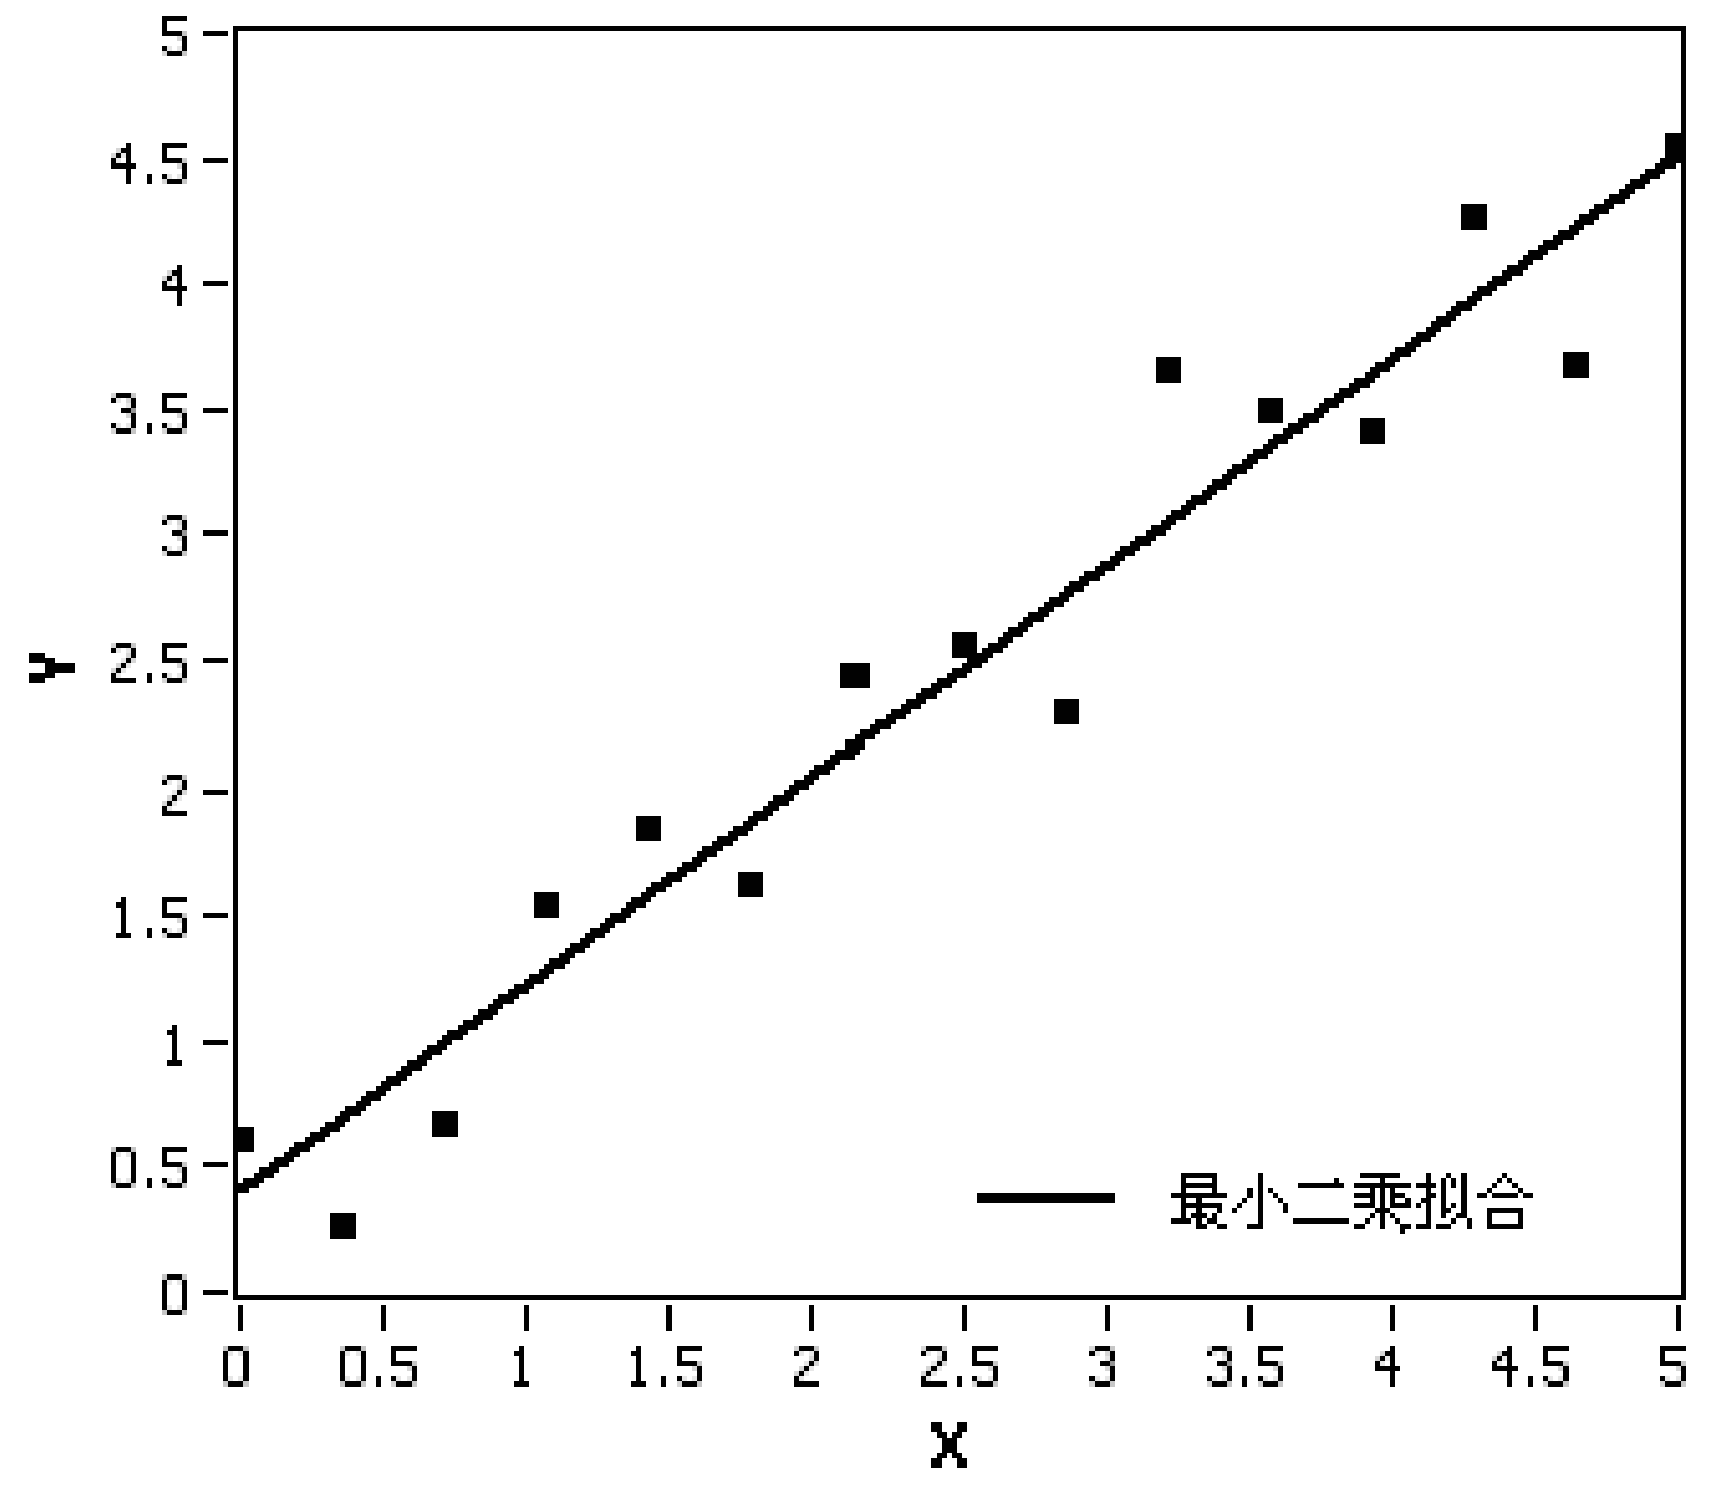
\includegraphics[width=10cm]{least_square_method}
%     \bicaption[fig:least_square_method]{最小二乘法统计示意图}{最小二乘法统计示意图}{Fig}{The least square method}
%   \end{minipage}     
% \end{figure}

% 而且,最小二乘法可以用作曲线拟合,由于在收集统计时序样本数据的时候,会得到波动的很多个点,这些点很难直接描述其变化特性,所以我们必须考虑用一种把现有数据透过数学方法来代入一条数式的表示方式,也就是采用最小二乘法,把收集到的无序样本组装成一条有意义的曲线,并根据这条曲线的数学特性来进行分析出样本值背后蕴含的统计意义。

% 在实际应用中,人们对由某一变量t或多个变量$t_{1}$……$t_{n}$ 构成的相关变量y感兴趣,如弹簧的形变与所用的力相关,一个企业的盈利与其营业额。为了得到这些变量同y之间的关系,便用不相关变量去构建y,使用如下函数模型中q个独立变量或p个系数去拟合。
% \begin {align}
% y_m = f(t_1,\dots, t_q;b_1,\dots,b_p),
% \end{align}
% 通常将一个对不相关变量t的构成无困难的函数类型叫做函数模型(例如抛物线函数)。其中参数b是用来使所选函数模型与观测值y匹配。合适地选择参数,使函数模型最好的拟合观测值。一般情况下,观测值远多于所选择的参数。

% \subsection{最小二乘算法实现}
在从时钟处,会不断收集离散的时延样本数据($t_{i}$, $D_{i}$)(i=1, 2, 3 $\cdots$),其中,$D_{i}$表示在从时钟$t_{i}$时刻获得的时延值。
为了进行最小二乘线性回归,取离当前最近的m个样本值来进行处理,并取基1,t,进行线性回归拟合
\begin {align}
f(t) = a_{0} + a_{1}t
\end{align}
使得方差值
\begin{align}
E(a_{0}, a_{1}) = \sum_{i=0}^{m}(f(t_{i}) - D_{i})^{2}
	= \sum_{i=0}^{m}(a_{0} + a_{1}t_{i} - D_{i})^{2}
\end{align}
能够达到极小值,因此,$a_{0}$ 和 $a_{1}$需要满足
\begin{align}
	\frac{\partial E}{\partial a_{k}} = 2 \sum_{i=0}^{m}t_{i}^{k}(a_{0} + a_{1}t_{i} - D_{i}) = 0
	\qquad(k = 0, 1)
\end{align}
上面的式子可以简化为如下形式:
\begin{align}
	a_{0}\sum_{i=0}^{m}t_{i}^{k} + a_{1}\sum_{i=0}^{m}t_{i}^{k+1} = \sum_{i=0}^{m}t_{i}^{k}D_{i}
	\qquad(k = 0, 1)
\end{align}
将该方程组转化为矩阵表示,可以得到如下的形式:
\begin{equation}
	\begin{bmatrix}
		m+1 & \sum_{i=0}^{m}t_{i} \\ 
		\sum_{i=0}^{m}t_{i} & \sum_{i=0}^{m}t_{i}^{2}
	\end{bmatrix}
	\begin{bmatrix}
	a_{0} \\ a_{1}
	\end{bmatrix}
	=
	\begin{bmatrix}
	 \sum_{i=0}^{m}D_{i} \\ \sum_{i=0}^{m}t_{i}D_{i}
	\end{bmatrix}
\end{equation}

将之前在从时钟所收集到的距当前最近的m个时延样本数据代入上述式子中,即利用方差最小原理,可以得到$a_{0}$ 和 $a_{1}$两个参数,因此便得到了一条拟合直线:f(t) = $a_{0}$ + $a_{1}$。此时就可以用该直线来估计当前时刻的真实时延时,而且,由于固有抖动噪声的随机性,通过该方法会显著消除时延抖动所造成的影响。

% \subsection{最小二乘算法优缺点分析}
针对链路延时固有抖动,由上文数学模型可以知道该抖动是属于随机变量,所以选择的思路是采用数学统计方法,把历史时延样本作为基础,通过对这些时延样本建立线性回归模型并得到一条拟合直线,通过该直线可以将随机扰动噪声造成的影响大大减下。

但是,对于同步系统中发生的暂时性突变,例如由堵塞等导致的暂时性的时延突变,若只是简单采用最小二乘法,那么时延的突变会导致回归直线的斜率快速增大,即导致计算出来的主从偏差也快速变化。当这种暂时性突变恢复正常,回归直线也逐渐恢复正常。这样容易导致从时钟经常处于快速振荡状态,非常不利于从时钟系统的正常工作。

所以,在下面将针对这种暂时性时延突变所带来危害进行限制,防止其突变造成主从偏差跟随性突变从而严重破坏从时钟鲁棒性。

\section{暂时性时延变化的动态阈值法}
由上文描述可以看出,单纯的最小二乘法确实可以有效的消除链路传输延时中的固有抖动部分,然而,一旦同步系统中发生由堵塞等导致的暂时性突变时,那么由最小二乘法回归得到的拟合直线也会随之有明显的突变,而这将导致相应的从时钟进行较大幅度的错误校正,而且,由于这种突变一般是暂时性的,所以,等网络负载恢复正常,拟合直线也渐渐恢复正常。然而,如果系统中频繁发生此类暂时性变化,那么势必会导致从时钟快速振荡。

因此,下文中针对暂时性时延变化作出深入研究,并且采用动态阈值法来应对此类暂时性变化的发生。

\subsection{暂时性时延变化特征研究}
对于堵塞等因素导致的暂时性时延变化$T_{q}(i)$,通过上文的数学模型分析可知,该时延变化因素是偶然性的,而且一般持续时间比较短,不过一旦出现,往往会导致时延出现较大的波动。可以将此类误差定义为暂时性阶跃噪声,一方面表示其持续时间较短,另一方面表示堵塞现象一旦发生,很有可能导致延时出现较大波动。

对从时钟而言,是采用上述最小二乘法来对历史时延进行线性回归估计,所以,如果出现了此类暂时性阶跃噪声,则会使的若干样本值相对旧有样本值之间,出现较大涨幅。而这种突变的涨幅会导致回归直线的斜率逐渐上升,则直接导致最终计算出来的延时值明显增大,从而导致$T_{offset}$值出现暂时性的大幅波动,虽然说后续随着网络负载的逐渐减轻而使的时延值及回归直线斜率逐渐恢复,但是,从从时钟稳定性角度出发,如果网络负载变化比较频繁,那么从时钟则会不断处于大幅波动之中,这对于从时钟系统稳定性极为不利。

\subsection{动态阈值法分析}
为了防止暂时性时延突变造成从时钟进入大幅波动甚至不稳定等现象,需要对时延变化进行一定的限制,或者说,通过历史时延的平均波动来衡量当前时延值带来的波动,如果当前时延值波动处于可接受阈值范围内则默认有效,若超过该阈值,则应该将其限制在阈值范围内。从而保证从时钟不会因为暂时性时延突变而出现快速大幅波动等不稳定现象。

对于阈值的选取,不应该将其设置为一个固定值,因为在网络环境不断变化的工业现场中人们无法提前预知堵塞等因素会导致的时延波动。所以,如果想要合理的判断当前时延的真实波动特性,最好的方法便是基于历史时延波动情况。如果当前时延波动与历史波动相比,处于一个有限范围内,那么可以认为当前时延带来的波动是正常的;反之,如果当前波动显著超过历史波动,那么应该对当前波动进行一定的限制,从而防止其对从时钟稳定性造成危害。

\subsection{动态阈值法实现}
由于动态阈值的计算需要实时根据历史时延波动数据而得。所以,为了能够计算历史波动情况,将首先创建一个固定时间窗,将每次的测量时延值保存其中;然后,通过时间窗内的历史时延值来计算时延波动阈值;最后,利用该阈值来衡量当前时延的抖动情况,并依据衡量结果来得到估计时延值。

下面给出一个含有测量时延和估计时延的固定时间窗,见表\ref{tab:dynamic_threshold}:
\begin{table}[!hpb]
  \centering
  \bicaption[tab:dynamic_threshold]{动态阈值法第k个固定时间窗}{动态阈值法第k个固定时间窗}{Table}{Mixed Time Window of Dynamic Threshold Method}
  \begin{tabular}{llllll} \toprule
  	时间 & $t_{k1}$ & $t_{k2}$ & $\cdots$ & $t_{k(m-1)}$ & $t_{km}$ \\ \midrule
    当前测量时延 & $d_{k1}$ & $d_{k2}$ & $\cdots$ & $d_{k(m-1)}$ & $d_{km}$ \\ \midrule
    动态阈值法时延估计值 & $\overline{D_{k1}}$ & $\overline{D_{k2}}$ & $\cdots$ & $\overline{D_{k(m-1)}}$ & $\overline{D_{km}}$  \\ \bottomrule
  \end{tabular}
\end{table}

其中,当前为时间$t_{ki}$,此时测量时延为$D_{ki}$,为了了解该时延的波动性,需要先计算历史时延的波动标准差,此时,假设之前的波动标准差为$\sigma_{i}$,该标准差可以直接对从$t_{k1}$时刻到$t_{k(i-1)}$时刻之间的估计时延,依据标准差公式计算而得。此处不作赘述。然后,可以依据该标准差$\sigma_{i}$来选取动态阈值,依据下式来进行选取:
\begin{align}
T_{i} = \alpha * \sigma_{i}
\end{align}
其中,$T_{i}$表示在$t_{ki}$根据历史时延数据实时计算出来的当前动态阈值,可以认为通过设定参数$\alpha$来调节阈值的范围,通常可取值为1 - 3。

然后,还需要引入截止函数来判断当前波动是否超出动态阈值的范围,并根据判断结果做出相应处理方法。将采用如下截止函数,当波动超过动态阈值时则直接取该阈值来计算当前实验估计值。
\begin{equation}
G(d_{i}) = \left\{
	\begin{array}{lll} % \begin{eqnarray}好像也可以。
		d_{i}, \qquad \left | d_{i} \right | < \alpha * \sigma_{i} \\
		\alpha * \sigma_{i}, \quad d_{i} \geq \alpha * \sigma_{i} \\
		-\alpha * \sigma_{i}, \quad d_{i} \leq -\alpha * \sigma_{i}
	\end{array}
	\alpha > 0 \right. 
\end{equation}

基于上面的动态阈值与截止函数,在$t_{ki}$时刻,可以利用第k个固定时间窗历史数据及当前测量延时$d_{i}$得到如下当前时延估计值:
\begin{align}
\overline{D_{ki}} = \gamma * G(d_{i}) + \overline{D_{k(i-1)}}; \qquad 1\leq i \leq m
\end{align}
其中,$\gamma$用来表示当前测量时延在当前估计时延$\overline{D_{ki}}$中所占的比重,一般可以取:
\begin{align}
\gamma \approx (0.85-0.9)
\end{align}
最后,每一轮时间窗的第一个延时估计值$\overline{D_{k1}}$是取上一轮时间窗所有时延估计值的平均值,即:
\begin{align}
\overline{D_{k1}} = \frac{1}{m} * \sum_{i=1}^{m}\overline{D_{(k-1)(i)}}
\end{align}

\subsection{动态阈值法优缺点分析}
利用上述动态阈值法,可以通过在固定时间窗内,通过计算历史时延值来得到一个动态阈值,然后利用该动态阈值来衡量当前测量时延的波动影响。若链路中发生较为严重的堵塞延时,导致时延值突然大幅增大,那么可以通过该动态阈值方法可以有效防止时延值大幅突变对从时钟造成的快速振荡甚至不稳定,从而使得从时钟有更加优良的稳定性。

但是,此方法的前提是该时延突变必须为暂时性突变,也就是说这种突变只是短时间内的,随着系统继续运行该突变又会逐渐减小并恢复正常。只有在这样的前提下,才可以通过动态阈值限定方法,在这个突变的短时间内把时延突变对从时钟造成的影响尽量减小。

然而,如果同步系统中发生的是持久性突变,例如拓扑结构变化,那么就意味着真实时延值与历史时延值已经完全不同,如果此时仍然采用上述动态阈值法强制把时延限制在一个有限范围内,那么很有可能导致数据完全偏离真实时延,出现难以想象的错误。

因此还需要针对同步系统中可能发生的持久性时延变化采用合适的方法来快速发现持久性突变的发生,并且采取相关措施以减小误差。

\section{持久性延时变化的滑动时间窗实时检测法}
\subsection{持久性延时变化特征研究}
虽然基于最小二乘法和动态阈值法可以有效的消除固定抖动噪声和暂时性阶跃噪声,改善了同步系统的精确性和鲁棒性。但是,如果发生由网络重配置等因素导致的拓扑结构变化时,就会导致链路传输时延的持久性变化,如果仅仅采用上述两种方法是无法有效应对此类变化的。

根本原因在于,一旦发生持久性变化,则意味着历史延时样本均已经失效,不应该继续用于后续的时延估计中。然而,上述两种方法均依赖于历史延时样本,而且这两种方法均无法探测出持久性变化的发生。这样带来的直接后果就是:在时延已经完全变化后,同步系统仍然继续使用错误的历史延时样本数据去估计当前真实的延时,所计算出来的估计时延值一定会与真实时延存在很大偏差,而且这样的偏差要一直持续到右足够多的新样本替代旧有时延样本后才能逐渐消除。

显然,这会严重破坏系统的同步精度和稳定性。因此,文中应用了一种基于固定滑动时间窗的实时检测法。

\subsection{滑动时间窗实时检测法}
这里所谓的持久性变化主要是指一旦发生了网络拓扑结构等变化,那么新的链路传输延时将与旧有延时样本完全不一致,这也就意味着,旧有累积延时样本已经不能作为计算新延时的基础数据了。否则,大量失效的延时样本数据会导致当前依靠最小二乘法所得到的时延估计出现非常严重的偏差。

所以,下面会上述最小二乘法所得到拟合直线斜率角度入手,来实时检测持久性变化的发生。

当从时钟收到同步报文时,会立即依靠历史数据和最小二乘法来建立一条回归直线。那么考虑这样一种情况,如果网络发生了重配置导致链路传输延时,那么此刻之后的新的延时数据就会与之前的样本数据有明显偏差,而此时仍然在使用最小二乘线性回归方法计算回归直线。那么可想而知,此刻之后的回归直线斜率会发生明显突变,假设网络重配置导致链路变得更长,那么得到的延时也就比之前更大,对应的回归直线斜率也会不断的向上提升,一直到历史实验样本全部被新的时延数据替代,那时的新的回归直线会恢复到接近水平。而在这个过程中,由于直线斜率的先增后减,导致其估计出来的时延值非常不准确,而且会导致从时钟发生一次大幅波动。

所以,理想的状态应该是,当发生拓扑结构突变,链路延时回归直线开始提升时,就能够尽快检测并发现这种现象,然后立即把历史时延数据失效化。从而,新的时延数据不会被历史样本影响而导致从时钟要经过长时间的波动直到新的时延完全替代旧有时延样本。于是,通过立即把历史时延数据失效的方法可以让从时钟尽快得到校正。

\subsection{滑动时间窗实时检测法实现}
这里需要着眼于回归直线斜率的变化情况,并通过对历史斜率的实时检测从而快速发现持久性变化的发生,并且采取使历史样本数据立即失效的方法来快速校正从时钟。为了能够实时检测回归直线的历史斜率变化情况,下面会采用滑动时间窗方法来实时检测并计算斜率变化。
\begin{table}[!hpb]
  \centering
  \bicaption[tab:slide_window]{实时检测法中在当前$t_{c}$时刻的长度为m的滑动时间窗}{在当前$t_{c}$时刻的滑动时间窗}{Table}{Slide Time Window at current time $t_{c}$ in Real-Time Monitor Method}
  \begin{tabular}{llllll} \toprule
  	时间 & $t_{c1}$ & $t_{c2}$ & $\cdots$ & $t_{c(m-1)}$ & $t_{cm}$ \\ \midrule
    当前测量时延 & $d_{c1}$ & $d_{c2}$ & $\cdots$ & $d_{(cm-1)}$ & $d_{cm}$ \\ \midrule
    当前回归直线斜率 & $\overline{K_{c1}}$ & $\overline{K_{c2}}$ & $\cdots$ & $\overline{K_{c(m-1)}}$ & $\overline{K_{cm}}$  \\ \bottomrule
  \end{tabular}
\end{table}

在表\ref{tab:slide_window}中,该时间窗最后一列数据为当前值。对应当前时刻为$t_{c}$,此时测量得到的时延值为$d_{c}$,同时可以得到当前回归直线的斜率值$\overline{K_{c}}$。由于如果当前同步系统并非发生持久性变化,那么该回归直线的斜率值应该是接近零并处于上下小幅抖动之中;而如果同步系统发生拓扑结构等持久性时延变化,那么斜率值则会处于一个不断上升或者不断下降的趋势之中。其中,不断上升意味着新的拓扑结构带来了更长的链路传输延时,反之,不断下降则意味着新拓扑结构带来了更短的链路传输延时。

那么,为了检测回归直线斜率的变化,下面从该滑动时间窗内的所有斜率样本值角度出发,通过探究这些斜率样本值的波动方差来决定是否发生持久性变化。即利用下面的式子来计算时间窗内的斜率均值$E_{c}$和方差$D_{c}$:
\begin{align}
E_{c} = \frac{1}{m}\sum_{i=1}^{m}(\overline{K_{ci}}) \\
D_{c} = \frac{1}{m}\sum_{i=1}^{m}(\overline{K_{ci}} - E_{c}) ^ {2}
\end{align}

所以,在$t_{c}$时刻可以计算出时间窗内的历史斜率波动方差为$D_{c}$,根据上文分析,若该方差接近零,则表示保持小幅振荡,此时可以认为没有发生持久性变化;但如果斜率方差值超过一定范围,那么可以认为同步系统中发生了持久性变化,为了使系统快速适应这种变化,则需要立即使历史样本失效。因此,采用下面函数来处理这种过程:
\begin{equation}
R_{c} = \left\{
	\begin{array}{ll} % \begin{eqnarray}好像也可以。
		0, \qquad D_{c} < \omega * \overline{DT} \\
		1, \quad D_{c} \geq \omega * \overline{DT} 
	\end{array}
	\right. 
\end{equation}
\begin{equation}
	\omega \approx (1 - 1.5)
\end{equation}
其中,$\omega$为可调节参数,也可以称为容忍度,即对于回归直线斜率变化的容忍程度,正常情况下,容忍度越小,则能够越快发现持久性变化。$\overline{DT}$为平均方差。若当前时间窗内所计算出来的波动超过了限定阈值,那么就认为发生了持久性变化,进行失效处理,即把所有旧有样本全部删除,并重新开始同步。从而保证从时钟对持久性变化的适应性和快速响应性。

对于滑动时间窗的实现,首先假设该时间窗长度为m,然后以最新测量时刻$t_{c}$的数据为该滑动时间窗的末尾一组数据,向前获取前(m-1)组数据加入该滑动时间窗内部。所以,每次新收到一次同步报文,便把该报文的数据加入到该滑动时间窗的最后一组,与此同时,将第一组数据从该时间窗内移除。所以整体看来,该时间窗是处于不断前行的一个过程,即每加入一个新样本则移除最早进入的样本,成为滑动时间窗。采用这样的方法可以时刻保持当前历史时延数据最新,才能够最快的检测出最真实的回归直线斜率的变动情况。

\subsection{滑动时间窗实时检测法小结}
首先,该方法主要是用来应对同步系统链路中发生的网络重配置等导致的拓扑结构变化。由于文章是从统计角度入手,所以每次同步计算都要严重依靠历史样本数据。而如果一旦发生了上述的持久性变化,那么就意味着历史样本数据已经完全失去效果了,如果继续使用则会导致严重误差且长时间无法正确校正。所以,本方法通过对时延的变化情况着手,通过实时检测最小二乘法中拟合直线的斜率变化,来快速判断同步系统中是否发生了持久性变化,一旦发现,便立即将历史样本失效,从而能够减小这种变化对同步系统造成的危害。

\section{本章小结}
本章首先从统计角度出发,对链路传输过程中可能导致时延变化的多个因素进行详细的分析,并且利用延时模型的特性,提供了一个系统性的同时应对多种链路延时波动因素的方法,即采用动态阈值法和滑动时间窗实时检测等方法来简便有效的应对固有抖动、暂时性时延突变和持久性时延变化等因素。这些方法都是基于历史实验样本数据,互相补充,能够完整而高效的应对复杂工业环境中同步系统链路延时的多种状况。不仅能提高从时钟的快速响应性和同步精度,还能改善从时钟的稳定性,使得同步系统能够更好应对拓扑结构变化和堵塞等现象。

%# -*- coding: utf-8-unix -*-
%%==================================================
%% chapter_4.tex for SJTU Master Thesis
%%==================================================

\chapter{基于数学统计策略来优化链路延时误差}
\section{链路延时不对称性分析及其对同步精度的影响}
\subsubsection{报文排队}
%# -*- coding: utf-8-unix -*-
%%==================================================
%% chapter_5.tex for SJTU Master Thesis
%%==================================================

\chapter{基于stateflow的PTP时钟同步仿真系统搭建及算法验证}

\section{仿真系统搭建及介绍}

\section{对链路时延的数学统计算法验证}

\section{对基于神经网络PID控制算法验证}

%# -*- coding: utf-8-unix -*-
%%==================================================
%% chapter_6.tex for SJTU Master Thesis
%%==================================================

\chapter{总结与展望}
行文至此,本人已经细致地对时钟同步技术及IEEE1588协议的相关问题进行了深入的研究和探讨,同时本人也创新性地从数学统计角度入手,提出了“动态阈值法”、“基于固定时间窗的实时动态监控算法”等,用来处理报文链路传输时延变化。同时也对于主从时钟源晶振漂移进行了分析,并从统计角度给出了相关的解决方案,而且通过文末的仿真能发现这些算法不仅能够在一定程度上提高系统的同步精度,而且能提高同步系统的稳定性和鲁棒性,对于工业环境下复杂的网络环境有良好的动态适应性。

下面,对于本文进行总结和展望。

\section{总结}
首先,由于当前分布式系统等应用越来越广泛,而其中时钟同步问题也已经成为了束缚分布式系统发展和实现很多实时性需求的一大瓶颈。而为了达到工业系统中所需要的时钟同步精度,我们通过分析了解发现遗忘的时钟同步方法如GPS、NTP、SNTP等技术均由于各种原因,如国防安全性、时钟同步精度和稳定性等,而无法满足当前工业环境对时钟同步的需求。而IEEE1588精密时钟同步协议由于其自身的易部署性、价格适中、同步精度高的多种特性使得其成为了当今非常重要且应用广泛的时钟同步技术。

然后,通过深入了解发现,IEEE1588时钟同步协议在实际运行中,并没有达到理想的微秒级甚至亚微秒级的时钟同步精度。于是,本人通过深入分析协议内容和实际运行背景,提炼出其中对同步精度破坏最大的两个因素:链路传输延时的随机性和变化性;从时钟校正策略。针对前者,本人创新性地从数学统计角度出发,把链路传输延时数据作为样本,并且根据其数学特性分别提出了“最小二乘线性回归算法”、“动态阈值法”和“基于固定时间窗的实时监控算法”等多种算法,分别对链路传输延时中的固有随机抖动、“暂时性”时延突变和“持久性”时延变化进行优化;然后,我们通过对主从时钟源晶振漂移进行了分析,提出了统计方法来进行补偿,另外还针对从时钟校正策略,从神经网络及PID控制角度出发,探索了这种控制策略的可行性。

在文章最后,我们利用stateflow工具,在matlab平台上搭建了一套完整的时钟同步仿真系统。本人利用该系统来对上文所提算法进行验证,通过最后的结果可以看出所提算法不仅能够改善同步系统的时钟同步精度,而且还能够充分应对链路中发生的由于拓扑结构变化等因素导致的“持久性”时延变化,这是当前很多同步算法并不具备的。除此之外,对于第四章对神经网络PID控制策略的可行性探究,我们也从仿真结果看出这种策略确实存在一定的应用价值和应用前景。

相信本人在上面所作的工作和研究成果,能够为之后的研究者提供一条不一样的思路,而且这些仿真结果能够为他们提供一定的实验依据。 

\section{展望}
在上文中,本人通过对IEEE1588时钟同步协议进行深入研究,发现了其中存在的严重问题,并且也提出了相应的解决方案,通过最后的仿真结果可以看出,这些方案确实能够改善同步系统的同步精度、稳定性和鲁棒性。

但是,这并不意味着这些方案已经没有缺陷了。

本人认为,后续的研究者可以从以下两个方面着手,进一步对本人所提的算法进行优化和改进以继续提高工业同步系统的同步精度和稳定性等指标。
\begin{enumerate}[noitemsep,topsep=0pt,parsep=0pt,partopsep=0pt]
	\item 由于本文针对链路延时是从数学统计角度出发进行研究,所以,这意味着从时钟必须能够存储一定数量的样本数据。当然,虽然这些数据都非常小,每个样本仅仅只是存储一个时延样本值,不过,对于存储空间有限的工业交换机设备而言,这些空间仍然是宝贵的,所以,后面可以探讨如何更有效的存储样本数据,如何及时把过时样本数据清空以保证硬件层能够有能力存储这些样本值;
	\item 对于时钟伺服系统,本文仅仅是从神经网络PID控制的角度进行了可行性验证,然后,具体的实现方法还有待改进。而且,神经网络的优势是能够对环境有很好的自适应性,这能够提供时钟同步系统对工业复杂网络环境的适应。但是,神经网络的缺陷是需要训练,而训练势必会导致较长的耗时,所以,如何衡量耗时和性能是一个重要的研究课题。
\end{enumerate}

最后,随着分布式系统和实时性需求的不断发展,时钟同步将会越来越影响到所有系统性能的关键一环,而当前实现时钟同步最有效的便是IEEE1588协议,因此对该协议的研究具有很广阔和长远的研究价值。而对协议而言,越来越高的时钟同步精度和系统稳定性将是持久的研究课题。
% %# -*- coding: utf-8-unix -*-
%%==================================================
%% chapter01.tex for SJTU Master Thesis
%%==================================================

\chapter{这是什么}
\label{chap:what}

这是上海交通大学(非官方)学位论文 \LaTeX 模板,当前版本是 \version 。

最早的一版学位模板是一位热心的物理系同学制作的。
那份模板参考了自动化所学位论文模板,使用了CASthesis.cls文档类,中文字符处理则采用当时最为流行的 \CJKLaTeX 方案。
我根据交大研究生院对学位论文的要求
\footnote{\url{http://www.gs.sjtu.edu.cn/policy/fileShow.ahtml?id=130}}
,结合少量个人审美喜好,完成了一份基本可用的交大 \LaTeX 学位论文模板。
但是,搭建一个 \CJKLaTeX 环境并不简单,单单在Linux下配置环境和添加中文字体,就足够让新手打退堂鼓。
在William Wang的建议下,我开始着手把模板向 \XeTeX 引擎移植。
他完成了最初的移植,多亏了他出色的工作,后续的改善工作也得以顺利进行。

随着我对 \LaTeX 系统认知增加,我又断断续续做了一些完善模板的工作,在原有硕士学位论文模板的基础上完成了交大学士和博士学位论文模板。

现在,交大学位论文模板SJTUTHesis代码在github
\footnote{\url{https://github.com/weijianwen/SJTUThesis}}
上维护。
你可以\href{https://github.com/weijianwen/SJTUThesis/issues}{在github上开issue}
、或者在\href{https://bbs.sjtu.edu.cn/bbsdoc?board=TeX_LaTeX}{水源LaTeX版}发帖来反映遇到的问题。

\section{使用模板}

\subsection{准备工作}
\label{sec:requirements}

要使用这个模板撰写学位论文,需要在\emph{TeX系统}、\emph{中英文字体}、\emph{TeX技能}上有所准备。

\begin{itemize}[noitemsep,topsep=0pt,parsep=0pt,partopsep=0pt]
	\item {\TeX}系统:所使用的{\TeX}系统要支持 \XeTeX 引擎,且带有ctex 2.x宏包,以2015年的\emph{完整}TeXLive、MacTeX发行版为佳。
	\item 中英文字体:操作系统中需要安装\footnote{在Windows、Mac OS X 以及 Linux 上安装额外的字体,可以参考\href{https://www.searchfreefonts.com/articles/how-to-install-fonts.htm}{“How to install fonts?”}。
}TeX Gyre Termes字体\footnote{\url{http://www.gust.org.pl/projects/e-foundry/tex-gyre/termes}}和四款Adobe中文字体
\footnote{请从合法渠道获得Adobe字体。}:AdobeSongStd、AdobeKaitiStd、AdobeHeitiStd、AdobeFangsongStd。
	\item TeX技能:尽管提供了对模板的必要说明,但这不是一份“ \LaTeX 入门文档”。在使用前请先通读其他入门文档。
	\item 针对Windows用户的额外需求:学位论文模本分别使用git和GNUMake进行版本控制和构建,建议从Cygwin\footnote{\url{http://cygwin.com}}安装这两个工具。
\end{itemize}

\subsection{模板选项}
\label{sec:thesisoption}

sjtuthesis提供了一些常用选项,在thesis.tex在导入sjtuthesis模板类时,可以组合使用。
这些选项包括:

\begin{itemize}[noitemsep,topsep=0pt,parsep=0pt,partopsep=0pt]
\item 学位类型:bachelor(学位)、master(硕士)、doctor(博士),是必选项。
\item 中国字体:adobefonts(Adobe中文字体)、winfonts(使用Windows下的中文字体,该选项未在Linux/Mac下测试)。
\item 正文字号:cs4size(小四)、c5size(五号)。
\item 盲审选项:使用review选项后,论文作者、学号、导师姓名、致谢、发表论文和参与项目将被隐去。
\end{itemize}

\subsection{编译模板}
\label{sec:process}

模板默认使用GNUMake构建,GNUMake将调用latemk工具自动完成模板多轮编译:

\begin{lstlisting}[basicstyle=\small\ttfamily, caption={编译模板}, numbers=none]
make clean thesis.pdf
\end{lstlisting}

若需要生成包含“原创性声明扫描件”的学位论文文档,请将扫描件保存为statement.pdf,然后调用make生成submit.pdf。

\begin{lstlisting}[basicstyle=\small\ttfamily, caption={生成用于提交的学位论文}, numbers=none]
make clean submit.pdf
\end{lstlisting}

编译失败时,可以尝试手动逐次编译,定位故障。

\begin{lstlisting}[basicstyle=\small\ttfamily, caption={手动逐次编译}, numbers=none]
xelatex -no-pdf thesis
biber --debug thesis
xelatex thesis
xelatex thesis
\end{lstlisting}

\subsection{模板文件布局}
\label{sec:layout}

\begin{lstlisting}[basicstyle=\small\ttfamily,caption={模板文件布局},label=layout,float,numbers=none]
├── LICENSE
├── Makefile
├── README.md
├── bib
│   └── thesis.bib
├── figure
│   ├── chap2
│   │   ├── sjtulogo.eps
│   │   ├── sjtulogo.jpg
│   │   ├── sjtulogo.pdf
│   │   └── sjtulogo.png
│   └── sjtubanner.png
├── sjtuthesis.cfg
├── sjtuthesis.cls
├── statement.pdf
├── submit.pdf
├── tex
│   ├── abstract.tex
│   ├── ack.tex
│   ├── app_cjk.tex
│   ├── app_eq.tex
│   ├── app_log.tex
│   ├── chapter01.tex
│   ├── chapter02.tex
│   ├── chapter03.tex
│   ├── conclusion.tex
│   ├── id.tex
│   ├── patents.tex
│   ├── projects.tex
│   ├── pub.tex
│   └── symbol.tex
└── thesis.tex
\end{lstlisting}

本节介绍学位论文模板中木要文件和目录的功能。

\subsubsection{格式控制文件}
\label{sec:format}

格式控制文件控制着论文的表现形式,包括两个文件: sjtuthesis.cfg, sjtuthesis.cls。

\subsubsection{主控文件thesis.tex}
\label{sec:thesistex}

主控文件thesis.tex的作用就是将你分散在多个文件中的内容“整合”成一篇完整的论文。
使用这个模板撰写学位论文时,你的学位论文内容和素材会被“拆散”到各个文件中:
譬如各章正文、各个附录、各章参考文献等等。
在thesis.tex中通过“include”命令将论文的各个部分包含进来,从而形成一篇结构完成的论文。
对模板定制时引入的宏包,建议放在导言区。

\subsubsection{各章源文件tex}
\label{sec:thesisbody}

这一部分是论文的主体,是以“章”为单位划分的,包括:

\begin{itemize}[noitemsep,topsep=0pt,parsep=0pt,partopsep=0pt]
	\item 中英文摘要(abstract.tex)。前言(frontmatter)的其他部分,中英文封面、原创性声明、授权信息在sjtuthesis.cls中定义,不单独分离为tex文件。
不单独弄成文件。
	\item 正文(mainmatter)——学位论文正文的各章内容,源文件是chapter\emph{xxx}.tex。
	\item 附录(app\emph{xx}.tex)、致谢(thuanks.tex)、攻读学位论文期间发表的学术论文目录(pub.tex)、个人简历(resume.tex)组成正文后的部分(backmatter)。
参考文献列表由biber插入,不作为一个单独的文件。
\end{itemize}

\subsubsection{图片文件夹figure}
\label{sec:fig}

figure文件夹放置了需要插入文档中的图片文件(支持PNG/JPG/PDF/EPS格式的图片),可以在按照章节划分子目录。
模板文件中使用\verb|\graphicspath|命令定义了图片存储的顶层目录,在插入图片时,顶层目录名“figure”可省略。

\subsubsection{参考文献数据库bib}
\label{sec:bib}

目前参考文件数据库目录只存放一个参考文件数据库thesis.bib。
关于参考文献引用,可参考第\ref{chap:example}章中的例子。


% %# -*- coding: utf-8-unix -*-
%%==================================================
%% chapter02.tex for SJTU Master Thesis
%% Encoding: UTF-8
%%==================================================

\chapter{ \LaTeX 排版例子}
\label{chap:example}

\section{数学排版}
\label{sec:matheq}

\subsection{公式排版}
\label{sec:eqformat}

这里有举一个长公式排版的例子,来自\href{http://www.tex.ac.uk/tex-archive/info/math/voss/mathmode/Mathmode.pdf}{《Math mode》}:

\begin {multline}
  \frac {1}{2}\Delta (f_{ij}f^{ij})=
  2\left (\sum _{i<j}\chi _{ij}(\sigma _{i}-
    \sigma _{j}) ^{2}+ f^{ij}\nabla _{j}\nabla _{i}(\Delta f)+\right .\\
  \left .+\nabla _{k}f_{ij}\nabla ^{k}f^{ij}+
    f^{ij}f^{k}\left [2\nabla _{i}R_{jk}-
      \nabla _{k}R_{ij}\right ]\vphantom {\sum _{i<j}}\right )
\end{multline}

\subsubsection{一个四级标题}
\label{sec:depth4}

这是全文唯一的一个四级标题。在这部分中将演示了mathtools宏包中可伸长符号(箭头、等号的例子)的例子。

\begin{displaymath}
    A \xleftarrow[n=0]{} B \xrightarrow[LongLongLongLong]{n>0} C 
\end{displaymath}

\begin{eqnarray}
  f(x) & \xleftrightarrow[]{A=B}  & B \\
  & \xleftharpoondown[below]{above} & B \nonumber \\
  & \xLeftrightarrow[below]{above} & B
\end{eqnarray}

又如:

\begin{align}
  \label{eq:none}
  & I(X_3;X_4)-I(X_3;X_4\mid{}X_1)-I(X_3;X_4\mid{}X_2) \nonumber \\
  = & [I(X_3;X_4)-I(X_3;X_4\mid{}X_1)]-I(X_3;X_4\mid{}\tilde{X}_2) \\
  = & I(X_1;X_3;X_4)-I(X_3;X_4\mid{}\tilde{X}_2)
\end{align}

\subsection{定理环境}

模板中定义了丰富的定理环境
algo(算法),thm(定理),lem(引理),prop(命题),cor(推论),defn(定义),conj(猜想),exmp(例),rem(注),case(情形),
bthm(断言定理),blem(断言引理),bprop(断言命题),bcor(断言推论)。
amsmath还提供了一个proof(证明)的环境。
这里举一个“定理”和“证明”的例子。
\begin{thm}[留数定理]
\label{thm:res}
  假设$U$是复平面上的一个单连通开子集,$a_1,\ldots,a_n$是复平面上有限个点,$f$是定义在$U\backslash \{a_1,\ldots,a_n\}$上的全纯函数,
  如果$\gamma$是一条把$a_1,\ldots,a_n$包围起来的可求长曲线,但不经过任何一个$a_k$,并且其起点与终点重合,那么:

  \begin{equation}
    \label{eq:res}
    \ointop_{\gamma}f(z)\,\mathrm{d}z = 2\uppi\mathbf{i}\sum^n_{k=1}\mathrm{I}(\gamma,a_k)\mathrm{Res}(f,a_k)
  \end{equation}

  如果$\gamma$是若尔当曲线,那么$\mathrm{I}(\gamma, a_k)=1$,因此:

  \begin{equation}
    \label{eq:resthm}
    \ointop_{\gamma}f(z)\,\mathrm{d}z = 2\uppi\mathbf{i}\sum^n_{k=1}\mathrm{Res}(f,a_k)
  \end{equation}

      % \oint_\gamma f(z)\, dz = 2\pi i \sum_{k=1}^n \mathrm{Res}(f, a_k ). 

  在这里,$\mathrm{Res}(f, a_k)$表示$f$在点$a_k$的留数,$\mathrm{I}(\gamma,a_k)$表示$\gamma$关于点$a_k$的卷绕数。
  卷绕数是一个整数,它描述了曲线$\gamma$绕过点$a_k$的次数。如果$\gamma$依逆时针方向绕着$a_k$移动,卷绕数就是一个正数,
  如果$\gamma$根本不绕过$a_k$,卷绕数就是零。

  定理\ref{thm:res}的证明。
  
  \begin{proof}
    首先,由……

    其次,……

    所以……
  \end{proof}
\end{thm}

上面的公式例子中,有一些细节希望大家注意。微分号d应该使用“直立体”也就是用mathrm包围起来。
并且,微分号和被积函数之间应该有一段小间隔,可以插入\verb+\,+得到。
斜体的$d$通常只作为一般变量。
i,j作为虚数单位时,也应该使用“直立体”为了明显,还加上了粗体,例如\verb+\mathbf{i}+。斜体$i,j$通常用作表示“序号”。
其他字母在表示常量时,也推荐使用“直立体”譬如,圆周率$\uppi$(需要upgreek宏包),自然对数的底$\mathrm{e}$。
不过,我个人觉得斜体的$e$和$\pi$很潇洒,在不至于引起混淆的情况下,我也用这两个字母的斜体表示对应的常量。


\section{向文档中插入图像}
\label{sec:insertimage}

\subsection{支持的图片格式}
\label{sec:imageformat}

\XeTeX 可以很方便地插入PDF、EPS、PNG、JPG格式的图片。

插入PNG/JPG的例子如\ref{fig:SRR}所示。
这两个水平并列放置的图共享一个“图标题”(table caption),没有各自的小标题。

\begin{figure}[!htp]
  \centering
  
\includegraphics[width=0.3\textwidth]{chap2/sjtulogo.png}
  \hspace{1cm}
  
\includegraphics[width=0.3\textwidth]{chap2/sjtulogo.jpg}
  \bicaption[fig:SRR]{这里将出现在插图索引中}{中文题图}{Fig}{English caption}
\end{figure}

这里还有插入eps图像和pdf图像的例子,如图\ref{fig:epspdf:a}和图\ref{fig:epspdf:b}。这里将EPS和PDF图片作为子图插入,每个子图有自己的小标题。并列子图的功能是使用subfigure宏包提供的。

\begin{figure}
  \centering
  \subfigure[EPS Figure]{
    \label{fig:epspdf:a} %% label for first subfigure
    
\includegraphics[width=0.3\textwidth]{chap2/sjtulogo.eps}}
  \hspace{1in}
  \subfigure[PDF Figure]{
    \label{fig:epspdf:b} %% label for second subfigure
    
\includegraphics[width=0.3\textwidth]{chap2/sjtulogo.pdf}}
  \bicaption[fig:pdfeps]{插入eps图像和pdf图像}{插入eps和pdf的例子}{Fig}{An EPS and PDF demo}
\end{figure}

更多关于 \LaTeX 插图的例子可以参考\href{http://www.cs.duke.edu/junhu/Graphics3.pdf}{《\LaTeX 插图指南》}。

\subsection{长标题的换行}
\label{sec:longcaption}

图\ref{fig:longcaptionbad}和图\ref{fig:longcaptiongood}都有比较长图标题,通过对比发现,图\ref{fig:longcaptiongood}的换行效果更好一些。
其中使用了minipage环境来限制整个浮动体的宽度。

\begin{figure}[!htp]
 \centering
 
\includegraphics[width=4cm]{chap2/sjtulogo.pdf}
 \bicaption[fig:longcaptionbad]{这里将出现在插图索引}{海交通大学是我国历史最悠久的高等学府之一,是教育部直属、教育部与上海市共建的全国重点大学.}{Fig}{Where there is a will, there is a way.}
\end{figure}

\begin{figure}[!hbp]
  \centering
  \begin{minipage}[b]{0.6\textwidth}
    \captionstyle{\centering}
    \centering
    
\includegraphics[width=4cm]{chap2/sjtulogo.pdf}
    \bicaption[fig:longcaptiongood]{这里将出现在插图索引}{海交通大学是我国历史最悠久的高等学府之一,是教育部直属、教育部与上海市共建的全国重点大学.}{Fig}{Where there is a will, there is a way.}
  \end{minipage}     
\end{figure}
  
\clearpage

\section{表格}
\label{sec:tab}

这一节给出的是一些表格的例子,如表\ref{tab:firstone}所示。

\begin{table}[!hpb]
  \centering
  \bicaption[tab:firstone]{指向一个表格的表目录索引}{一个颇为标准的三线表格\footnotemark[1]}{Table}{A Table}
  \begin{tabular}{@{}llr@{}} \toprule
    \multicolumn{2}{c}{Item} \\ \cmidrule(r){1-2}
    Animal & Description & Price (\$)\\ \midrule
    Gnat & per gram & 13.65 \\
    & each & 0.01 \\
    Gnu & stuffed & 92.50 \\
    Emu & stuffed & 33.33 \\
    Armadillo & frozen & 8.99 \\ \bottomrule
  \end{tabular}
\end{table}
\footnotetext[1]{这个例子来自\href{http://www.ctan.org/tex-archive/macros/latex/contrib/booktabs/booktabs.pdf}{《Publication quality tables in LATEX》}(booktabs宏包的文档)。这也是一个在表格中使用脚注的例子,请留意与threeparttable实现的效果有何不同。}

下面一个是一个更复杂的表格,用threeparttable实现带有脚注的表格,如表\ref{tab:footnote}。

\begin{table}[!htpb]
  \bicaption[tab:footnote]{出现在表目录的标题}{一个带有脚注的表格的例子}{Table}{A Table with footnotes}
  \centering
  \begin{threeparttable}[b]
     \begin{tabular}{ccd{4}cccc}
      \toprule
      \multirow{2}{6mm}{total}&\multicolumn{2}{c}{20\tnote{1}} & \multicolumn{2}{c}{40} &  \multicolumn{2}{c}{60}\\
      \cmidrule(lr){2-3}\cmidrule(lr){4-5}\cmidrule(lr){6-7}
      &www & k & www & k & www & k \\
      \midrule
      &$\underset{(2.12)}{4.22}$ & 120.0140\tnote{2} & 333.15 & 0.0411 & 444.99 & 0.1387 \\
      &168.6123 & 10.86 & 255.37 & 0.0353 & 376.14 & 0.1058 \\
      &6.761    & 0.007 & 235.37 & 0.0267 & 348.66 & 0.1010 \\
      \bottomrule
    \end{tabular}
    \begin{tablenotes}
    \item [1] the first note.% or \item [a]
    \item [2] the second note.% or \item [b]
    \end{tablenotes}
  \end{threeparttable}
\end{table}

\section{参考文献管理}

 \LaTeX 具有将参考文献内容和表现形式分开管理的能力,涉及三个要素:参考文献数据库、参考文献引用格式、在正文中引用参考文献。
这样的流程需要多次编译:

\begin{enumerate}[noitemsep,topsep=0pt,parsep=0pt,partopsep=0pt]
	\item 用户将论文中需要引用的参考文献条目,录入纯文本数据库文件(bib文件)。
	\item 调用xelatex对论文模板做第一次编译,扫描文中引用的参考文献,生成参考文献入口文件(aux)文件。
	\item 调用biber,以参考文献格式和入口文件为输入,生成格式化以后的参考文献条目文件(bib)。
	\item 再次调用xelatex编译模板,将格式化以后的参考文献条目插入正文。
\end{enumerate}

参考文献数据库(thesis.bib)的条目,可以从Google Scholar搜索引擎\footnote{\url{https://scholar.google.com}}、CiteSeerX搜索引擎\footnote{\url{http://citeseerx.ist.psu.edu}}中查找,文献管理软件Papers\footnote{\url{http://papersapp.com}}、Mendeley\footnote{\url{http://www.mendeley.com}}、JabRef\footnote{\url{http://jabref.sourceforge.net}}也能够输出条目信息。

下面是在Google Scholar上搜索到的一条文献信息,格式是纯文本:

\begin{lstlisting}[caption={从Google Scholar找到的参考文献条目}, label=googlescholar, float, escapeinside="", numbers=none]
    @phdthesis{"白2008信用风险传染模型和信用衍生品的定价",
      title={{"信用风险传染模型和信用衍生品的定价"}},
      author={"白云芬"},
      year={2008},
      school={"上海交通大学"}
    } 
\end{lstlisting}

为了方便引用,建议将文献别名改用ASCII表示。
中文文献的处理有别于英文文献,对中文参考文献需要增加“language”域显式说明。

\begin{lstlisting}[caption={修改后的参考文献条目}, label=itemok, float, escapeinside="", numbers=none]
  @phdthesis{bai2008,
    title={{"信用风险传染模型和信用衍生品的定价"}},
    author={"白云芬"},
    year={2008},
    language={chinese},
    address={"上海"},
    school={"上海交通大学"}
  } 
\end{lstlisting}

按照教务处的要求,参考文献外观应符合国标GBT7714的要求\footnote{\url{http://www.cces.net.cn/guild/sites/tmxb/Files/19798_2.pdf}}。
在本模板中,我们使用caspervector\footnote{\url{http://www.ctan.org/pkg/biblatex-caspervector}}参考文献样式,这是一种非常接近GB风格,但在美学细节上更优秀的风格。

正文中引用参考文献时,用\verb+\supercite{key1,key2,key3...}+可以产生“上标引用的参考文献”,
如\supercite{Meta_CN,chen2007act,DPMG}。
使用\verb+\parencite{key1,key2,key3...}+则可以产生水平引用的参考文献,例如\parencite{JohnD,zhubajie,IEEE-1363}。
请看下面的例子,将会穿插使用水平的和上标的参考文献:关于书的\parencite{Meta_CN,JohnD,IEEE-1363},关于期刊的\supercite{chen2007act,chen2007ewi},
会议论文\parencite{DPMG,kocher99,cnproceed},
硕士学位论文\parencite{zhubajie,metamori2004},博士学位论文\supercite{shaheshang,FistSystem01,bai2008},标准文件\parencite{IEEE-1363},技术报告\supercite{NPB2},电子文献\parencite{xiaoyu2001, CHRISTINE1998},用户手册\parencite{RManual}。

总结一些注意事项:
\begin{itemize}[noitemsep,topsep=0pt,parsep=0pt,partopsep=0pt]
\item 参考文献只有在正文中被引用了,才会在最后的参考文献列表中出现;
\item 参考文献“数据库文件”bib是纯文本文件,请使用UTF-8编码,不要使用GBK编码;
\item 参考文献条目中通过language域是否为空判断是否是中文文献;
\end{itemize}

\section{用listings插入源代码}

原先ctexbook文档类和listings宏包配合使用时,代码在换页时会出现莫名其妙的错误,后来经高人指点,顺利解决了。
感兴趣的话,可以看看\href{http://bbs.ctex.org/viewthread.php?tid=53451}{这里}。
这里给使用listings宏包插入源代码的例子,这里是一段C代码。
另外,listings宏包真可谓博大精深,可以实现各种复杂、漂亮的效果,想要进一步学习的同学,可以参考
\href{http://mirror.ctan.org/macros/latex/contrib/listings/listings.pdf}{listings宏包手册}。

\begin{lstlisting}[language={C}, caption={一段C源代码}]
#include <stdio.h>
#include <unistd.h>
#include <sys/types.h>
#include <sys/wait.h>

int main() {
  pid_t pid;

  switch ((pid = fork())) {
  case -1:
    printf("fork failed\n");
    break;
  case 0:
    /* child calls exec */
    execl("/bin/ls", "ls", "-l", (char*)0);
    printf("execl failed\n");
    break;
  default:
    /* parent uses wait to suspend execution until child finishes */
    wait((int*)0);
    printf("is completed\n");
    break;
  }

  return 0;
}
\end{lstlisting}

\section{用algorithm和algorithmic宏包插入算法描述}

如算法\ref{algo:sum_I_want}所示。

\begin{algorithm}
\caption{求和算法}
\label{algo:sum_I_want}
\begin{algorithmic}
\REQUIRE $n \geq 1$                  %输入条件
\ENSURE $Sum = 1 + \cdots + n$       %输出
\STATE $Sum \leftarrow 0$            %\STATE 命名演示
\IF {$n < 1$}                        %条件语句
\PRINT {Input Error}                 %打印语句
\ENDIF
\RETURN Sum
\end{algorithmic}
\end{algorithm}


% %# -*- coding: utf-8-unix -*-
\chapter{常见问题}
\label{chap:faq}

{\bfseries{}Q:我是否能够自由使用这份模板?}

A:这份模板以Apache License 2.0开源许可证发布,请遵循许可证规范。

{\bfseries{}Q:我的论文是Word排版的,学校图书馆是不是只收 \LaTeX 排版的论文?}

A:当然不是,Word版论文肯定收。

{\bfseries{}Q:我的论文是 \LaTeX 排版的,学校图书馆是不是只收Word排版的论文?}

A:当然不是,PDF版的电子论文是可以上交的。是否要交Word版就看你导师的喜好了。

{\bfseries{}Q:为什么屏幕上显示的左右页边距不一样?}

A:模板默认是双面打印,迎面页和背面页的页边距是要交换的,多出来的那一部分是留作装订的。

{\bfseries{}Q:如何获得帮助和反馈意见?}

A:你可以通过\href{https://github.com/weijianwen/sjtu-thesis-template-latex/issues}{在github上开issue}
、在\href{https://bbs.sjtu.edu.cn/bbsdoc?board=TeX_LaTeX}{水源LaTeX版}发帖反映你使用过程中遇到的问题。

{\bfseries{}Q:使用文本编辑器查看tex文件时遇到乱码?}

A:请确保你的文本编辑器使用UTF-8编码打开了tex源文件。

{\bfseries{}Q:在CTeX编译模板遇到“rsfs10.tfm already exists”的错误提示?}

A:请删除\verb+X:\CTEX\UserData\fonts\tfm\public\rsfs+下的文件再重新编译。问题讨论见\href{https://bbs.sjtu.edu.cn/bbstcon,board,TeX_LaTeX,reid,1352982719.html}{水源2023号帖}。

{\bfseries{}Q:升级了TeXLive 2012,编译后的文档出现“minus”等字样?}

A:这是xltxtra和fontspec宏包导致的问题。学位论文模板从0.5起使用metatlog宏包代替xltxtra生成 \XeTeX 标志,解决了这个问题。

{\bfseries{}Q:为什么在bib中加入的参考文献,没有在参考文献列表中出现?}

A: bib中的参考文献条目,只有通过\verb+\parencite+或者\verb+\supercite+在正文中引用,才会加入到参考文献列表中。

{\bfseries{}Q:在macTex中,为什么pdf图片无法插入?}

A:如果报错是“pdf: image inclusion failed for "./figure/chap2/sjtulogo.pdf".”,则采取以下步骤

\begin{lstlisting}[basicstyle=\small\ttfamily, caption={编译模板}, numbers=none]
  brew install xpdf
  wget http://mirrors.ctan.org/support/epstopdf.zip
  unzip epstopdf.zip
  cp epstopdf/epstopdf.pl /usr/local/bin/
  cd figure/chap2
  pdftops sjtulogo.pdf
  epstopdf sjtulogo.ps
  pdfcrop sjtulogo.pdf
  mv sjtulogo.pdf backup.pdf
  mv sjtulogo-crop.pdf sjtulogo.pdf
\end{lstlisting}

{\bfseries{}Q:如何向你致谢?}

A: 烦请在模板的\href{https://github.com/weijianwen/SJTUThesis}{github主页}点击“Star”,我想粗略统计一下使用学位论文模板的人数,谢谢大家。非常欢迎大家向项目贡献代码。

%# -*- coding: utf-8-unix -*-
%%==================================================
%% conclusion.tex for SJTUThesis
%% Encoding: UTF-8
%%==================================================

\begin{summary}
研究生期间,在导师带领下,本人开始逐步接触时钟同步技术和IEEE1588精密时钟同步协议。在了解中发现,目前工业领域越来越多的应用了IEEE1588精密时钟同步协议来提高分布式系统的同步性能,所以也在研究学习中对时钟同步技术和IEEE1588协议本身产生兴趣。然后通过不断的阅读各种文献和深入阅读IEEE1588协议内容,对时钟同步技术有了全面的了解。

不过,慢慢就发现了IEEE1588精密时钟同步协议在实际应用中仍然存在的很多缺陷和问题。正是这些问题的存在导致了实际的运行效果不尽如人意,其同步精度也往往很难达到理想的目标。因此,决定着手深入研究这些问题的根源及其解决方案。

在导师的指引下,文章中创新性地从数学统计角度来深入分析这些问题,并且提出了一套自己的解决方案,这一套统计算法覆盖了报文固有抖动、排队堵塞等导致的暂时性时延突变、拓扑结构变化导致的持久性时延变化和从时钟频率漂移等多种破坏同步精度的因素。最后,通过搭建的stateflow仿真平台上对所提算法进行验证,可以发现这些算法不仅能有效提高系统的同步精度,还能改善同步系统应对复杂工业环境的稳定性和自适应性。

然后,通过这篇论文的撰写,又重新梳理了之前的思路,并试图以尽可能准确的语言和描述把之前的研究工作及成果展示给大家。同时,也将研究过程进行记录,以方面后续的研究人员在此基础上能够继续探究,不断改良时钟同步系统的精度,使得IEEE1588协议能够发挥其理想的效果,具备更大的实际应用价值。

最后,通过对时钟同步技术的研究,我也培养了自身的科研习惯,能够从更加理性的角度去思考问题,也学会了通过阅读国内外文献来扩展自己的视野和优化自己的思维方式。另外,这个过程也让我感受到了科研的魅力,受益匪浅。相信以后能够继续保持这种谨慎认真的态度来面对未来的工作和学习。

\end{summary}


\appendix	% 使用英文字母对附录编号,重新定义附录中的公式、图图表编号样式
\renewcommand\theequation{\Alph{chapter}--\arabic{equation}}	
\renewcommand\thefigure{\Alph{chapter}--\arabic{figure}}
\renewcommand\thetable{\Alph{chapter}--\arabic{table}}
\renewcommand\thealgorithm{\Alph{chapter}--\arabic{algorithm}}

%% 附录内容,本科学位论文可以用翻译的文献替代。
% %# -*- coding: utf-8-unix -*-
\chapter{搭建模板编译环境}

\section{安装TeX发行版}

\subsection{Mac OS X}

Mac用户可以从MacTeX主页\footnote{\url{https://tug.org/mactex/}}下载MacTeX 2015。
也可以通过brew包管理器\footnote{\url{http://caskroom.io}}安装MacTeX 2015。

\begin{lstlisting}[basicstyle=\small\ttfamily, numbers=none]
brew cask install mactex
\end{lstlisting}

\subsection{Linux}

建议Linux用户使用TeXLive主页\footnote{\url{https://www.tug.org/texlive/}}的脚本来安装TeXLive 2015。
以下命令将把TeXLive发行版安装到当前用户的家目录下。
若计划安装一个供系统上所有用户使用的TeXLive,请使用root账户操作。

\begin{lstlisting}[basicstyle=\small\ttfamily, numbers=none]
wget http://mirror.ctan.org/systems/texlive/tlnet/install-tl-unx.tar.gz
tar xzvpf install-tl-unx.tar.gz
cd install-tl-20150411/
./install-tl
\end{lstlisting}

\section{安装中文字体}

\subsection{Mac OS X、Deepin}

Mac和Deepin用户双击字体文件即可安装字体。

\subsection{RedHat/CentOS用户}

RedHat/CentOS用户请先将字体文件复制到字体目录下,调用fc-cache刷新缓存后即可在TeXLive中使用新字体。

\begin{lstlisting}[basicstyle=\small\ttfamily, numbers=none]
mkdir ~/.fonts
cp *.ttf ~/.fonts				# 当前用户可用新字体
cp *.ttf /usr/share/fonts/local/	# 所有用户可以使用新字体
fc-cache -f
\end{lstlisting}


% %# -*- coding: utf-8-unix -*-
%% app2.tex for SJTU Master Thesis
%% based on CASthesis
%% modified by wei.jianwen@gmail.com
%% version: 0.3a
%% Encoding: UTF-8
%% last update: Dec 5th, 2010
%%==================================================

\chapter{Maxwell Equations}

选择二维情况,有如下的偏振矢量:
\begin{subequations}
  \begin{eqnarray}
    {\bf E}&=&E_z(r,\theta)\hat{\bf z} \\
    {\bf H}&=&H_r(r,\theta))\hat{ \bf r}+H_\theta(r,\theta)\hat{\bm
      \theta}
  \end{eqnarray}
\end{subequations}
对上式求旋度:
\begin{subequations}
  \begin{eqnarray}
    \nabla\times{\bf E}&=&\frac{1}{r}\frac{\partial E_z}{\partial\theta}{\hat{\bf r}}-\frac{\partial E_z}{\partial r}{\hat{\bm\theta}}\\
    \nabla\times{\bf H}&=&\left[\frac{1}{r}\frac{\partial}{\partial
        r}(rH_\theta)-\frac{1}{r}\frac{\partial
        H_r}{\partial\theta}\right]{\hat{\bf z}}
  \end{eqnarray}
\end{subequations}
因为在柱坐标系下,$\overline{\overline\mu}$是对角的,所以Maxwell方程组中电场$\bf E$的旋度:
\begin{subequations}
  \begin{eqnarray}
    &&\nabla\times{\bf E}=\mathbf{i}\omega{\bf B} \\
    &&\frac{1}{r}\frac{\partial E_z}{\partial\theta}{\hat{\bf
        r}}-\frac{\partial E_z}{\partial
      r}{\hat{\bm\theta}}=\mathbf{i}\omega\mu_rH_r{\hat{\bf r}}+\mathbf{i}\omega\mu_\theta
    H_\theta{\hat{\bm\theta}}
  \end{eqnarray}
\end{subequations}
所以$\bf H$的各个分量可以写为:
\begin{subequations}
  \begin{eqnarray}
    H_r=\frac{1}{\mathbf{i}\omega\mu_r}\frac{1}{r}\frac{\partial
      E_z}{\partial\theta } \\
    H_\theta=-\frac{1}{\mathbf{i}\omega\mu_\theta}\frac{\partial E_z}{\partial r}
  \end{eqnarray}
\end{subequations}
同样地,在柱坐标系下,$\overline{\overline\epsilon}$是对角的,所以Maxwell方程组中磁场$\bf H$的旋度:
\begin{subequations}
  \begin{eqnarray}
    &&\nabla\times{\bf H}=-\mathbf{i}\omega{\bf D}\\
    &&\left[\frac{1}{r}\frac{\partial}{\partial
        r}(rH_\theta)-\frac{1}{r}\frac{\partial
        H_r}{\partial\theta}\right]{\hat{\bf
        z}}=-\mathbf{i}\omega{\overline{\overline\epsilon}}{\bf
      E}=-\mathbf{i}\omega\epsilon_zE_z{\hat{\bf z}} \\
    &&\frac{1}{r}\frac{\partial}{\partial
      r}(rH_\theta)-\frac{1}{r}\frac{\partial
      H_r}{\partial\theta}=-\mathbf{i}\omega\epsilon_zE_z
  \end{eqnarray}
\end{subequations}
由此我们可以得到关于$E_z$的波函数方程:
\begin{eqnarray}
  \frac{1}{\mu_\theta\epsilon_z}\frac{1}{r}\frac{\partial}{\partial r}
  \left(r\frac{\partial E_z}{\partial r}\right)+
  \frac{1}{\mu_r\epsilon_z}\frac{1}{r^2}\frac{\partial^2E_z}{\partial\theta^2}
  +\omega^2 E_z=0
\end{eqnarray}

% %# -*- coding: utf-8-unix -*-
\chapter{从 \CJKLaTeX 转向 \XeTeX }
\label{chap:whydvipdfm}

我习惯把v0.2a使用dvipdfmx编译的硕士学位论文模板称为“ \CJKLaTeX 模板”,而这个使用 \XeTeX 引擎(xelatex程序)处理的模板则被称为“{\XeTeX/\LaTeX}模板”。
从 \CJKLaTeX 模板迁移到{\XeTeX\LaTeX}模板的好处有下:
\begin{enumerate}
\item[\large\smiley] 搭建 \XeTeX 环境比搭建 \CJKLaTeX 环境更容易;
\item[\large\smiley] 更简单的字体控制;
\item[\large\smiley] 完美支持PDF/EPS/PNG/JPG图片,不需要“bound box(.bb)”文件;
\item[\large\smiley] 支持OpenType字体的复杂字型变化功能;
\end{enumerate}

当然,这也是有代价的。由于 \XeTeX 比较新,在我看来,使用 \XeTeX 模板所必须付出的代价是:

\begin{enumerate}
\item[\large\frownie] 必须把你“古老的” \TeX 系统更新为较新的版本。TeXLive 2012和CTeX 2.9.2能够编译这份模板,而更早的版本则无能为力。
\item[\large\frownie] 需要花一些时间把你在老模板上的工作迁移到新模板上。
\end{enumerate}

第一条就看你如何取舍了,新系统通常意味着更好的兼容性,值得升级。而转换模板也不是什么特别困难的事情,可以这样完成:

\begin{enumerate}
\item 备份你要转换的源文件,以防你的工作成果丢失;
\item 将你原来的tex以及bib文件另存为UTF-8编码的文件。iconv、vim、emacs、UEdit等等工具都可以完成。WinEdt对文件编码识别功能很差(到了v6.0还是如此),不推荐作为字符编码转换工具;
\item 将diss.tex导言区中的内容替换为XeTeX模板diss.tex导言区的内容;
\item 将你对原先导言区的修改,小心翼翼地合并到新的导言区中;
\item 使用XeTeX模板中的GBT7714-2005NLang.bst替换原有的bst文件,新的bst文件只是将字符编码转换为UTF-8;
\item 删除bouding box文件;
\item 使用本文\ref{sec:process}介绍的方法,重新编译文档;
\end{enumerate}


% %# -*- coding: utf-8-unix -*-
\chapter{模板更新记录}
\label{chap:updatelog}

\textbf{2015年6月19日} v0.9发布,适配ctex 2.x宏包,需要使用TeXLive 2015编译。

\textbf{2015年3月15日} v0.8发布,使用biber/biblatex组合替代 \BibTeX ,带来更强大稳定的参考文献处理能力;添加enumitem宏包增强列表环境控制能力;完善宏包文字描述。

\textbf{2015年2月15日} v0.7发布,增加盲审选项,调用外部工具插入扫描件。

\textbf{2015年2月14日} v0.6.5发布,修正一些小问题,缩减git仓库体积,仓库由sjtu-thesis-template-latex更名为SJTUThesis。

\textbf{2014年12月17日} v0.6发布,学士、硕士、博士学位论文模板合并在了一起。

\textbf{2013年5月26日} v0.5.3发布,更正subsubsection格式错误,这个错误导致如"1.1 小结"这样的标题没有被正确加粗。

\textbf{2012年12月27日} v0.5.2发布,更正拼写错误。在diss.tex加入ack.tex。

\textbf{2012年12月21日} v0.5.1发布,在 \LaTeX 命令和中文字符之间留了空格,在Makefile中增加release功能。

\textbf{2012年12月5日} v0.5发布,修改说明文件的措辞,更正Makefile文件,使用metalog宏包替换xltxtra宏包,使用mathtools宏包替换amsmath宏包,移除了所有CJKtilde(\verb+~+)符号。

\textbf{2012年5月30日} v0.4发布,包含交大学士、硕士、博士学位论文模板。模板在\href{https://github.com/weijianwen/sjtu-thesis-template-latex}{github}上管理和更新。

\textbf{2010年12月5日} v0.3a发布,移植到 \XeTeX/\LaTeX 上。

\textbf{2009年12月25日} v0.2a发布,模板由CASthesis改名为sjtumaster。在diss.tex中可以方便地改变正文字号、切换但双面打印。增加了不编号的一章“全文总结”。
添加了可伸缩符号(等号、箭头)的例子,增加了长标题换行的例子。

\textbf{2009年11月20日} v0.1c发布,增加了Linux下使用ctex宏包的注意事项、.bib条目的规范要求,
修正了ctexbook与listings共同使用时的断页错误。

\textbf{2009年11月13日} v0.1b发布,完善了模板使用说明,增加了定理环境、并列子图、三线表格的例子。

\textbf{2009年11月12日} 上海交通大学硕士学位论文 \LaTeX 模板发布,版本0.1a。



\backmatter	% 文后无编号部分 

%% 参考资料
\printbibliography[heading=bibintoc]

%% 致谢、发表论文、申请专利、参与项目、简历
%% 用于盲审的论文需隐去致谢、发表论文、申请专利、参与的项目
\makeatletter
\ifsjtu@review\relax\else
  %# -*- coding: utf-8-unix -*-
\begin{thanks}

在交大研究生的这两年时间里,我从一名从没接触过科研的普通学生起步,开始接触交大优秀的教师,并在研一期间学习了非常多自己感兴趣的知识,而每一堂课的老师都能够耐心回答我所提出的疑惑,使得本人的知识面有了非常大的拓宽。所以我很感谢交大有一批优秀的教师为我们传道解惑。

进入实验室后,开始跟随导师完成实验室的项目,依次接触过软件验证、核电电路图绘制和时钟同步技术研究等多个工作。在这些工作中,导师通过不断指导给予了我很多帮助,也让我从一名初学者逐渐学习提高。尤其是在时钟同步技术方面的深入研究历程极大提高了我的科研能力,让我感受到了作为一名科研工作者应有的认真和谨慎。所以非常感谢导师对我的耐心传授和方向指引,使得我真正感受到作为一名研究生的价值。

然后,还要感谢父母在读研期间对自己的关心和鼓励,尤其是当自己生病时陪伴左右。这些都是本人不断前进的动力来源。另外,实验室的师兄弟们也给予了我很多的关心和帮助,我也要感谢他们对本人的照顾和帮助。

最后,感谢交大这所学校,本人在这里感受到了一所综合学府的学术、上进和踏实,也在这里完成了本科生到研究生的蜕变。

无论是从心智还是情感,这里的收获都将让我受益匪浅。

感谢!
\end{thanks}
 	  %% 致谢
  %# -*- coding: utf-8-unix -*-
%%==================================================
%% pub.tex for SJTUThesis
%% Encoding: UTF-8
%%==================================================

\begin{publications}{99}
    \item\textsc{第一作者}. {统计方法在IEEE1588时钟同步协议中的应用}. 化工自动化及仪表, 2015.07.
\end{publications}
	  %% 发表论文
  % %# -*- coding: utf-8-unix -*-
\begin{patents}{99}
    \item 第一发明人,“永动机”,专利申请号202510149890.0
\end{patents}
	  %% 申请专利
  % %# -*- coding: utf-8-unix -*-
%%==================================================
%% projects.tex for SJTUThesis
%% Encoding: UTF-8
%%==================================================

\begin{projects}{99}
    \item 973项目“XXX”
    \item 自然基金项目“XXX”
    \item 国防项目“XXX”
\end{projects}
  %% 参与的项目
% \include{tex/resume}	  %% 各人简历
\fi
\makeatother

\end{document}
